\documentclass[aspectratio=1610]{beamer}

\usetheme{KTH}
\usepackage{caption}
\captionsetup[figure]{labelformat=empty}% redefines the caption setup of the figures environment in the beamer class.
\captionsetup[subfigure]{labelformat=empty}

\input{/home/peter/Organisatorisches/Latex_dinge/packages_beamer}

\addbibresource{/home/peter/EasterIslands/Literature/EasterIslandbib.bib}

\usepackage{appendixnumberbeamer}

\addtobeamertemplate{navigation symbols}{}{%
	\usebeamerfont{footline}%
	\usebeamercolor[fg]{footline}%
	\hspace{5em}%
	\insertframenumber/\inserttotalframenumber
}

\usepackage{mwe}

\usepackage{multimedia}
\usepackage{media9}

\author{Peter Steiglechner}
\title{Easter Island ABM}
\subtitle{Masterthesis Presentation Defence}
\institute{ZMT Bremen}
\date{\today}

% remove this if using XeLaTeX or LuaLaTeX
\usepackage[utf8]{inputenc}
\usepackage{wasysym}

\usepackage[ruled,vlined]{algorithm2e}

\AtBeginSection[]
{
	\begin{frame}[noframenumbering]{Outline}
	\begin{Large}\begin{center}
			\textbf{A Spatially Explicit Agent-Based Model \\ for Human-Resource Interaction on Easter Island}
	\end{center}\end{Large}
	\tableofcontents[currentsection]
\end{frame}
}

\begin{document}
	
	\startpage
	%%%%%%%%%%%%%%%%%%%%%%%%%%%%%%%%%%%%%%%%%%%%%%%%%%%%%%%%%%%%
	\begin{frame}[noframenumbering]
	
	\vspace{0.02\textheight}
	\begin{Large}\begin{center}
		\textbf{A Spatially Explicit Agent-Based Model \\ for Human-Resource Interaction on Easter Island}
\end{center}\end{Large}
	\vspace{0.01\textheight}

	\begin{small}
		\begin{center}
		En Rumsligt Explicit Agentbaserad Modell av Interaktionen mellan Människor och Resurser på Påskön
		\end{center}

	\end{small}
	
	\vspace{0.02\textheight}
	
	\begin{small}
		\begin{center}
		\textit{Peter Steiglechner, 29 June 2020}
		\end{center}

	\end{small}
\end{frame}


\normalpage


\begin{frame}[noframenumbering]
\frametitle{Outline}
	\begin{Large}\begin{center}
	\textbf{A Spatially Explicit Agent-Based Model \\ for Human-Resource Interaction on Easter Island}
	\end{center}\end{Large}
\tableofcontents
\end{frame}



\section{Easter Island History}
% !TEX root = presentation_29Jun.tex


\begin{frame}{Easter Island Mystery}
	\centering
	\begin{columns}
		\begin{column}{0.7\textwidth}
				\includegraphics[width=\linewidth]{../../EIMap_Merico2017}
			\captionof{figure}{\citet{Merico2017}}
		\end{column}
	\pause\begin{column}{0.3\textwidth}
	\centering
	\includegraphics[width=0.7\linewidth]{../../Diamond2011Cover}
	\captionof{figure}{\citet{Diamond2011}}
	\end{column}
	\end{columns}
\end{frame}

\begin{frame}{Facts of Easter Island History}
\centering
%\begin{itemize}
%	\item Forest
%	\item Polynesian Rats
%	\item Intensified deforestation from $1200\, {\rm A.D.}$ in many locations
%	\item Intensified farming (with the use of lithic mulching)
%	\item Moai statues carved between $1200$ and $1700 \, {\rm A.D.}$
%	\item European voyages arrive in $1722$, $1770$s, ... and introduce European diseases and slave trade (especially in the 19th century)
%\end{itemize}
%But: Pollen and Charcoal data is scarce and difficult to interpret.
\begin{figure}
	\centering
	\begin{subfigure}{0.15\textwidth}
	\centering
	\only<1-6>{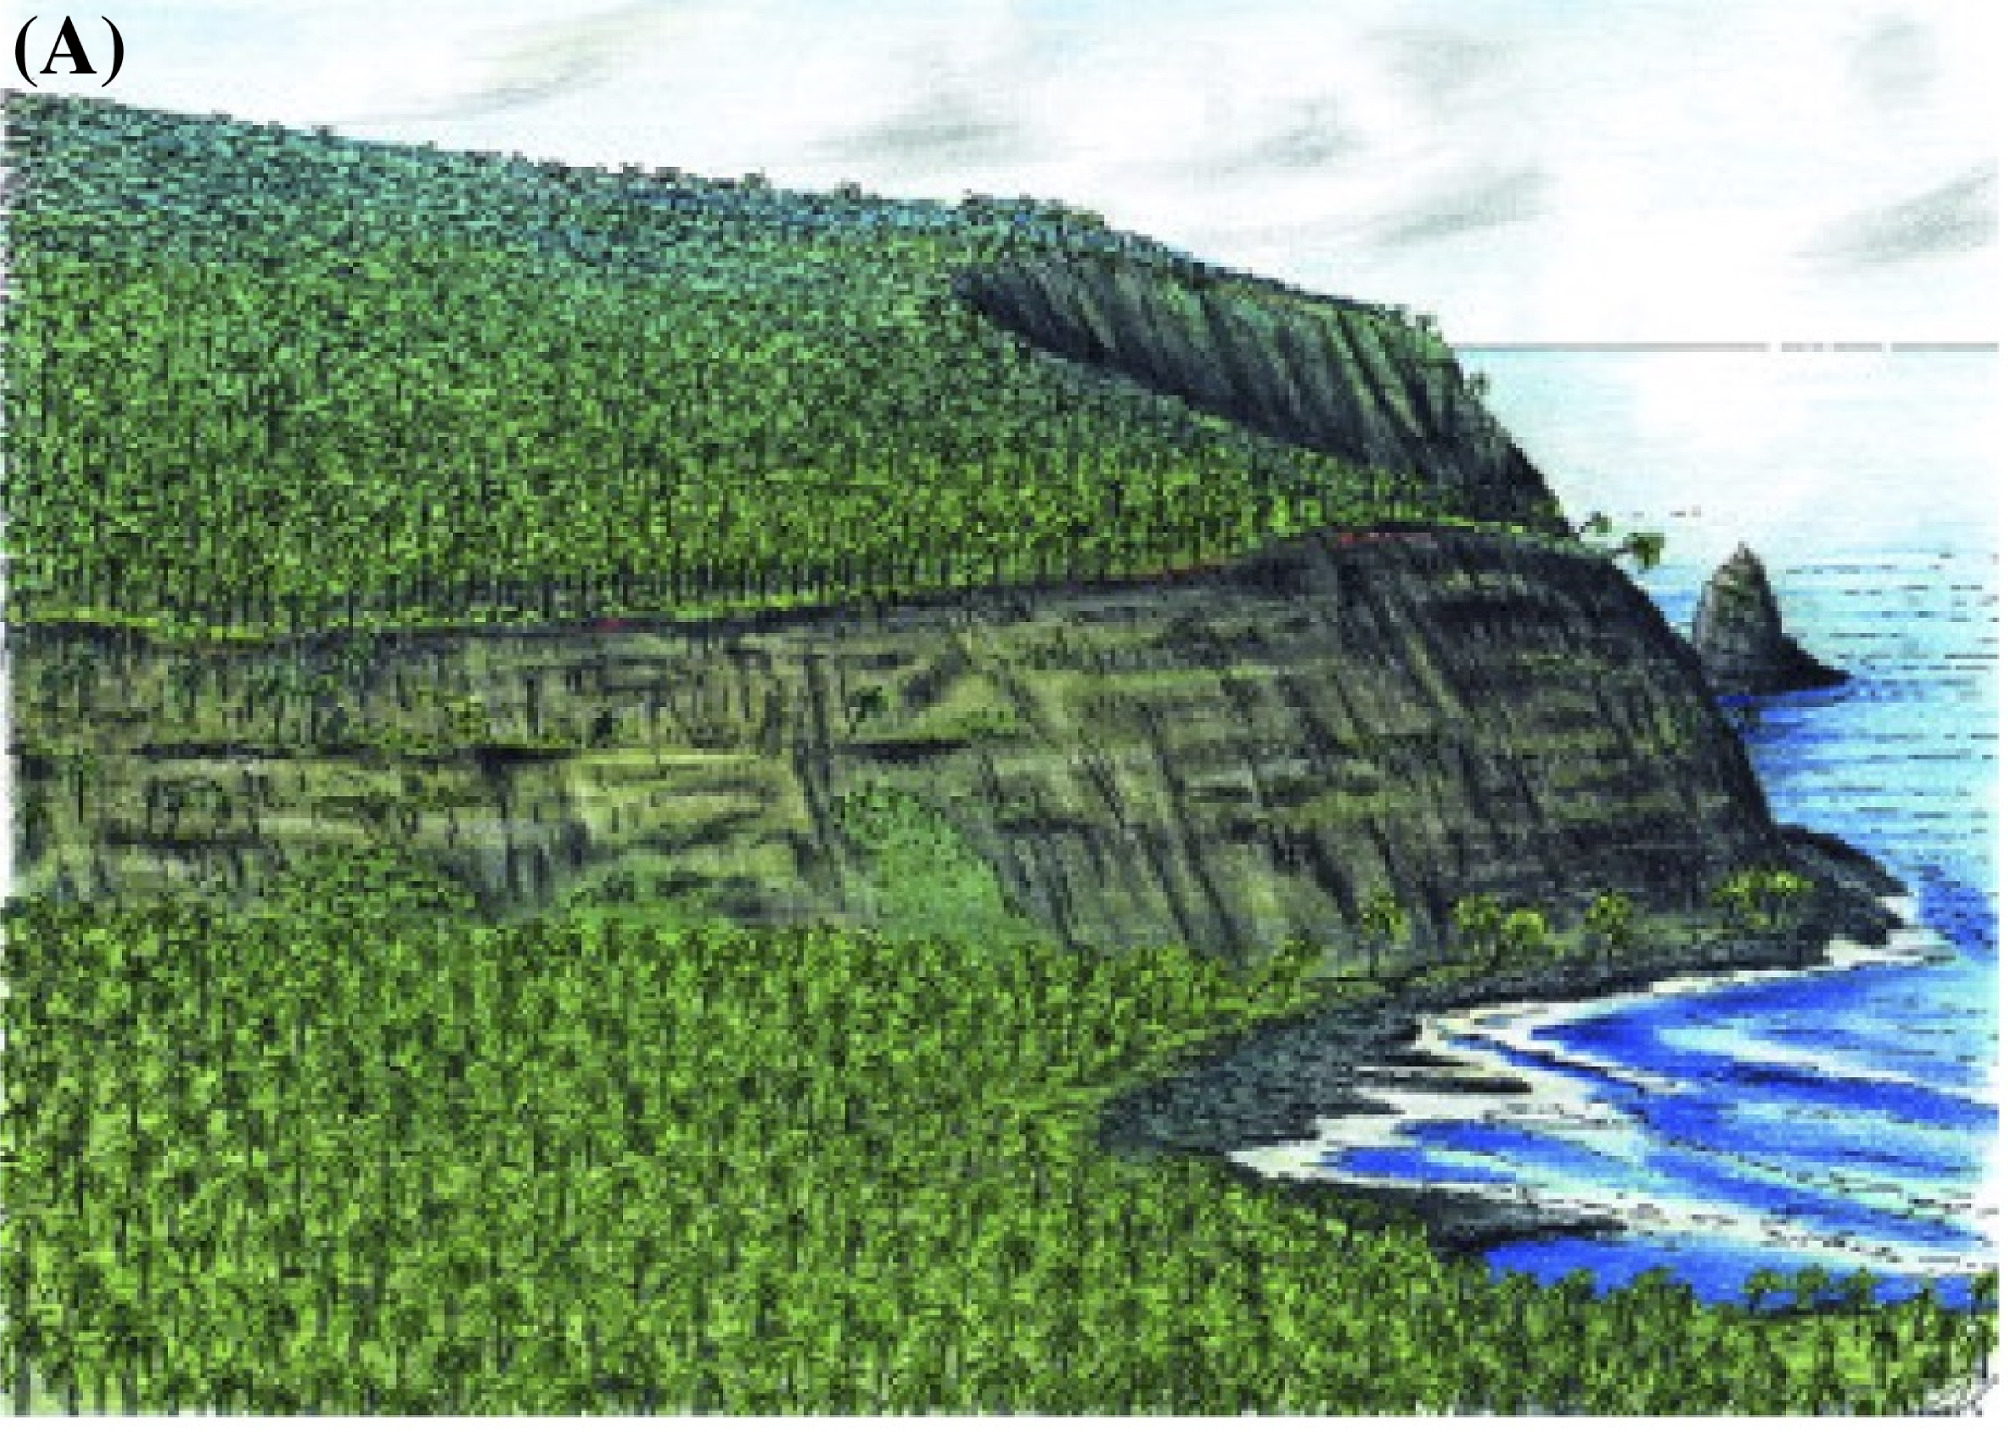
\includegraphics[height=1cm]{images/ForestGerdCloseRull2020.jpg}
	\caption{{\scriptsize Palm Forest }}}
	\end{subfigure}\hfill
	\begin{subfigure}{0.15\textwidth}
	\centering
	\only<1-6>{	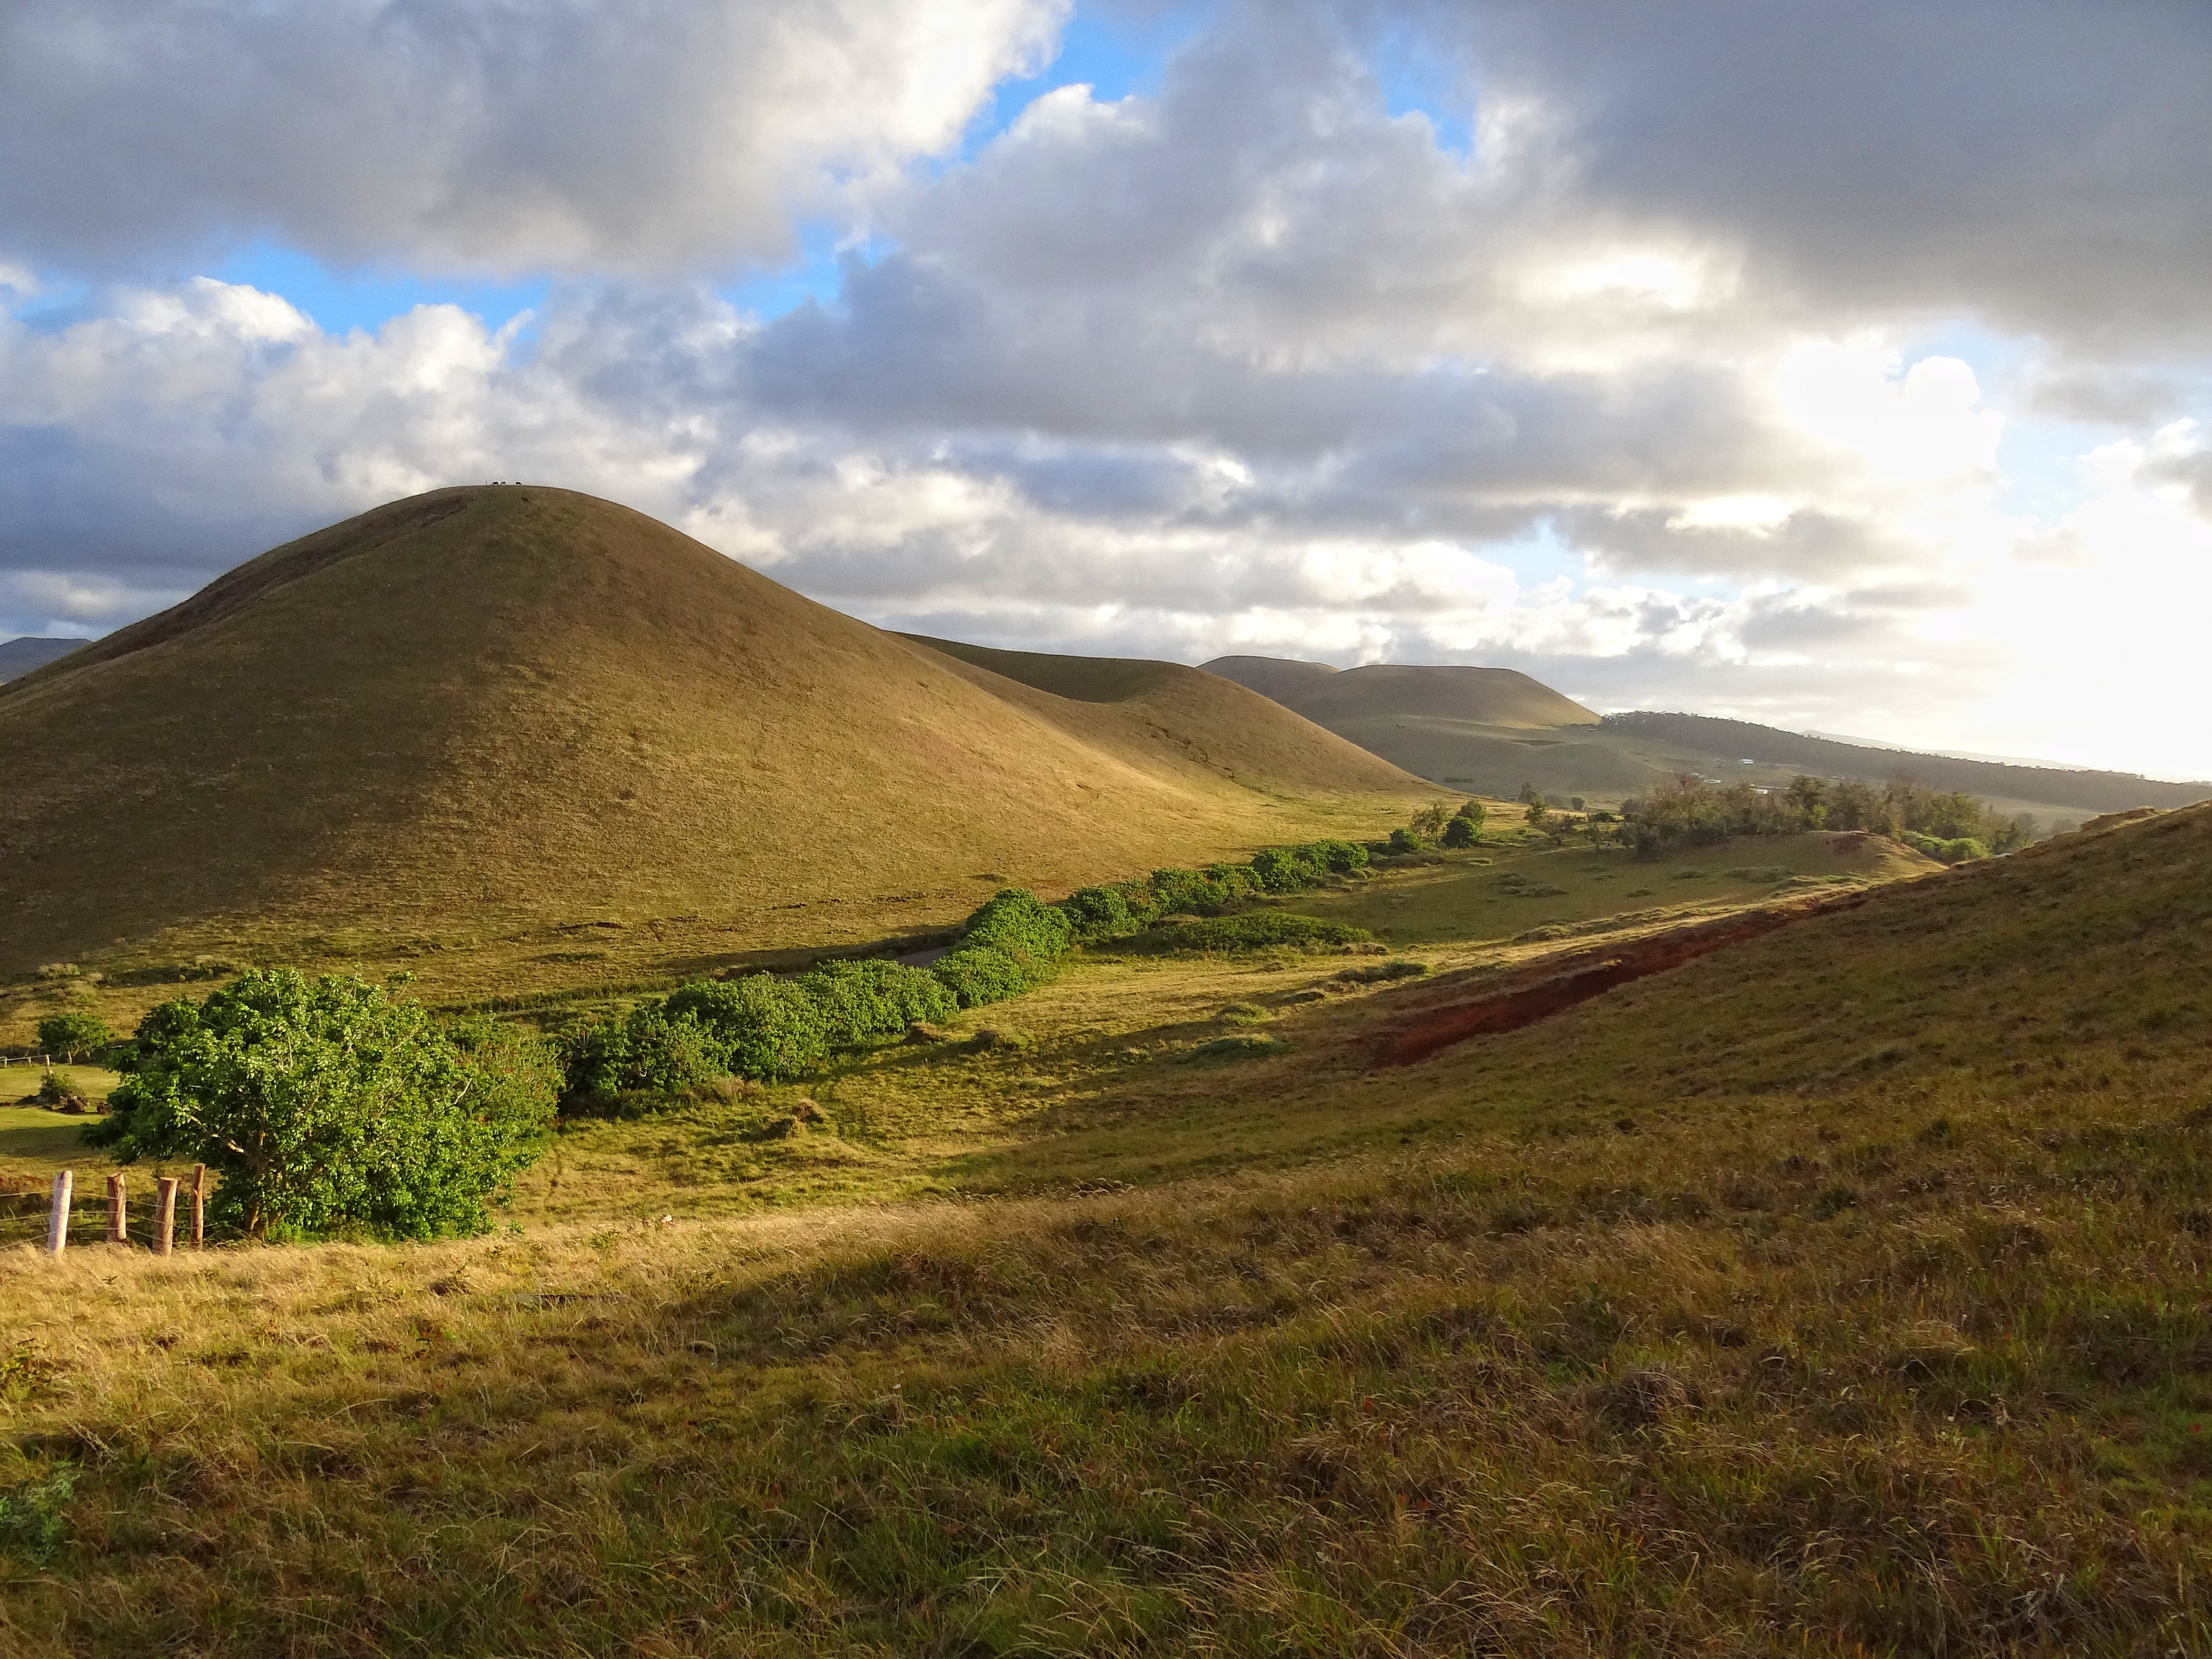
\includegraphics[height=1cm]{images/Rapa-Nui-Landscape.jpg}
	\caption{{\scriptsize Deforestation}}}
	\end{subfigure}\hfill
	\begin{subfigure}{0.15\textwidth}
	\centering
	\only<1-6>{	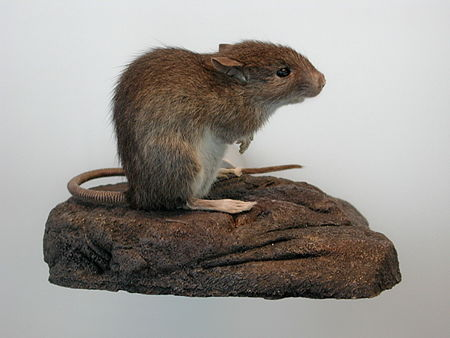
\includegraphics[height=1cm]{images/Pacific_rat.jpg}
		\caption{{\scriptsize Pacific Rats}}}
	\end{subfigure}\hfill
	\begin{subfigure}{0.15\textwidth}
	\centering
	\only<1-6>{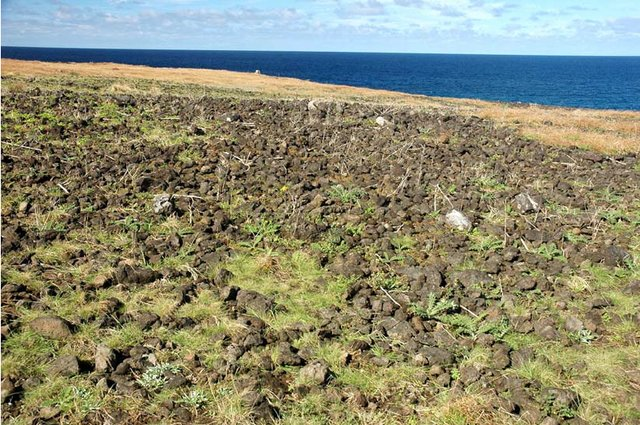
\includegraphics[height=1cm]{images/lithicMulching.jpg}
	\caption{{\scriptsize Agriculture}}}
	\end{subfigure}\hfill
	\begin{subfigure}{0.15\textwidth}
	\centering
	\only<1-6>{	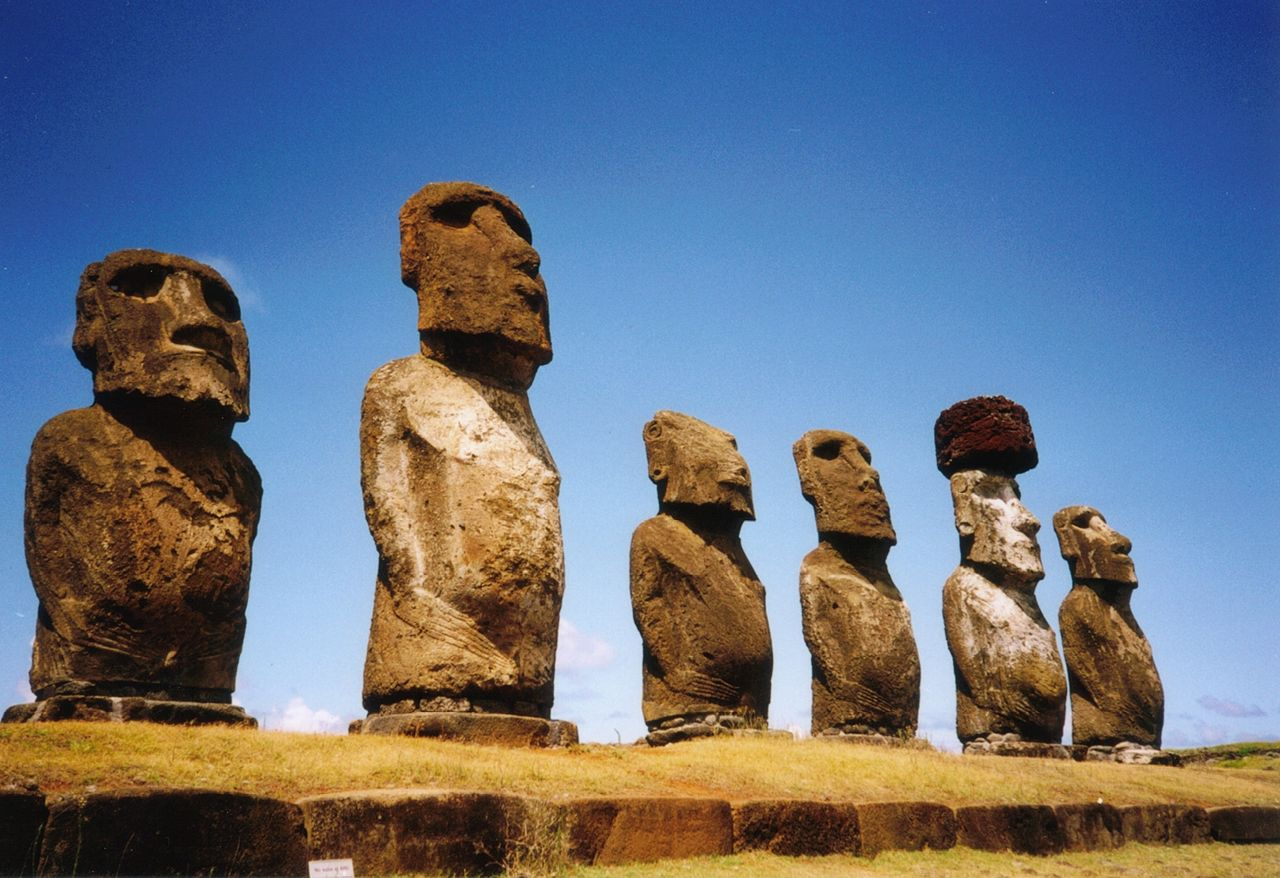
\includegraphics[height=1cm]{images/moai3.jpg}
	\caption{{\scriptsize Moai Statues}}}
	\end{subfigure}\hfill
	\begin{subfigure}{0.18\textwidth}
	\centering			\only<1-6>{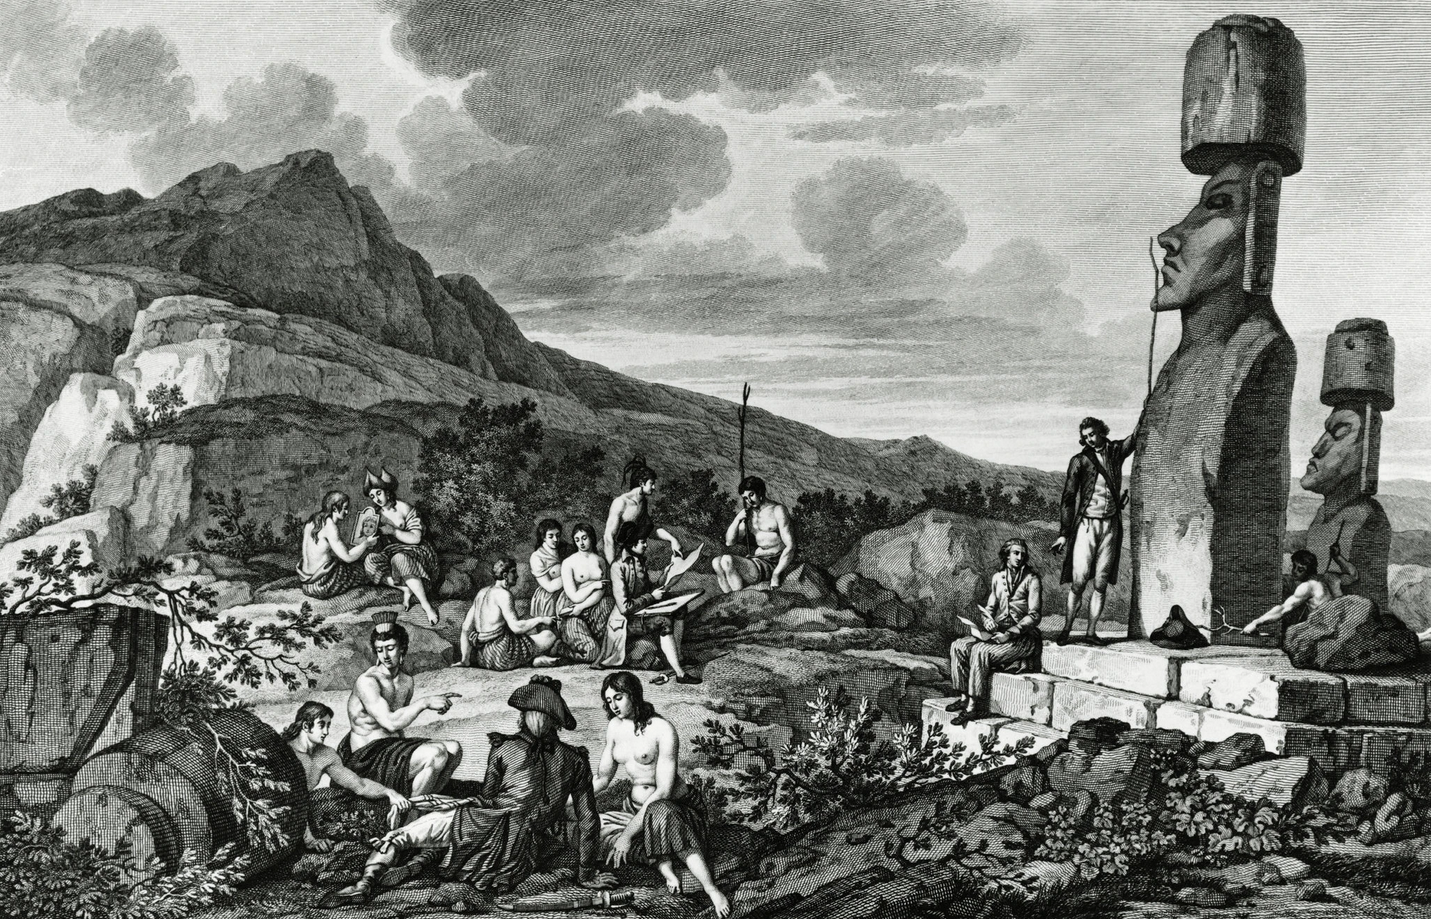
\includegraphics[height=1cm]{images/voyages.png}
	\caption{{\scriptsize European Contact}}}
	\end{subfigure}
\end{figure}
%
\begin{figure}
	\centering
	\only<1>{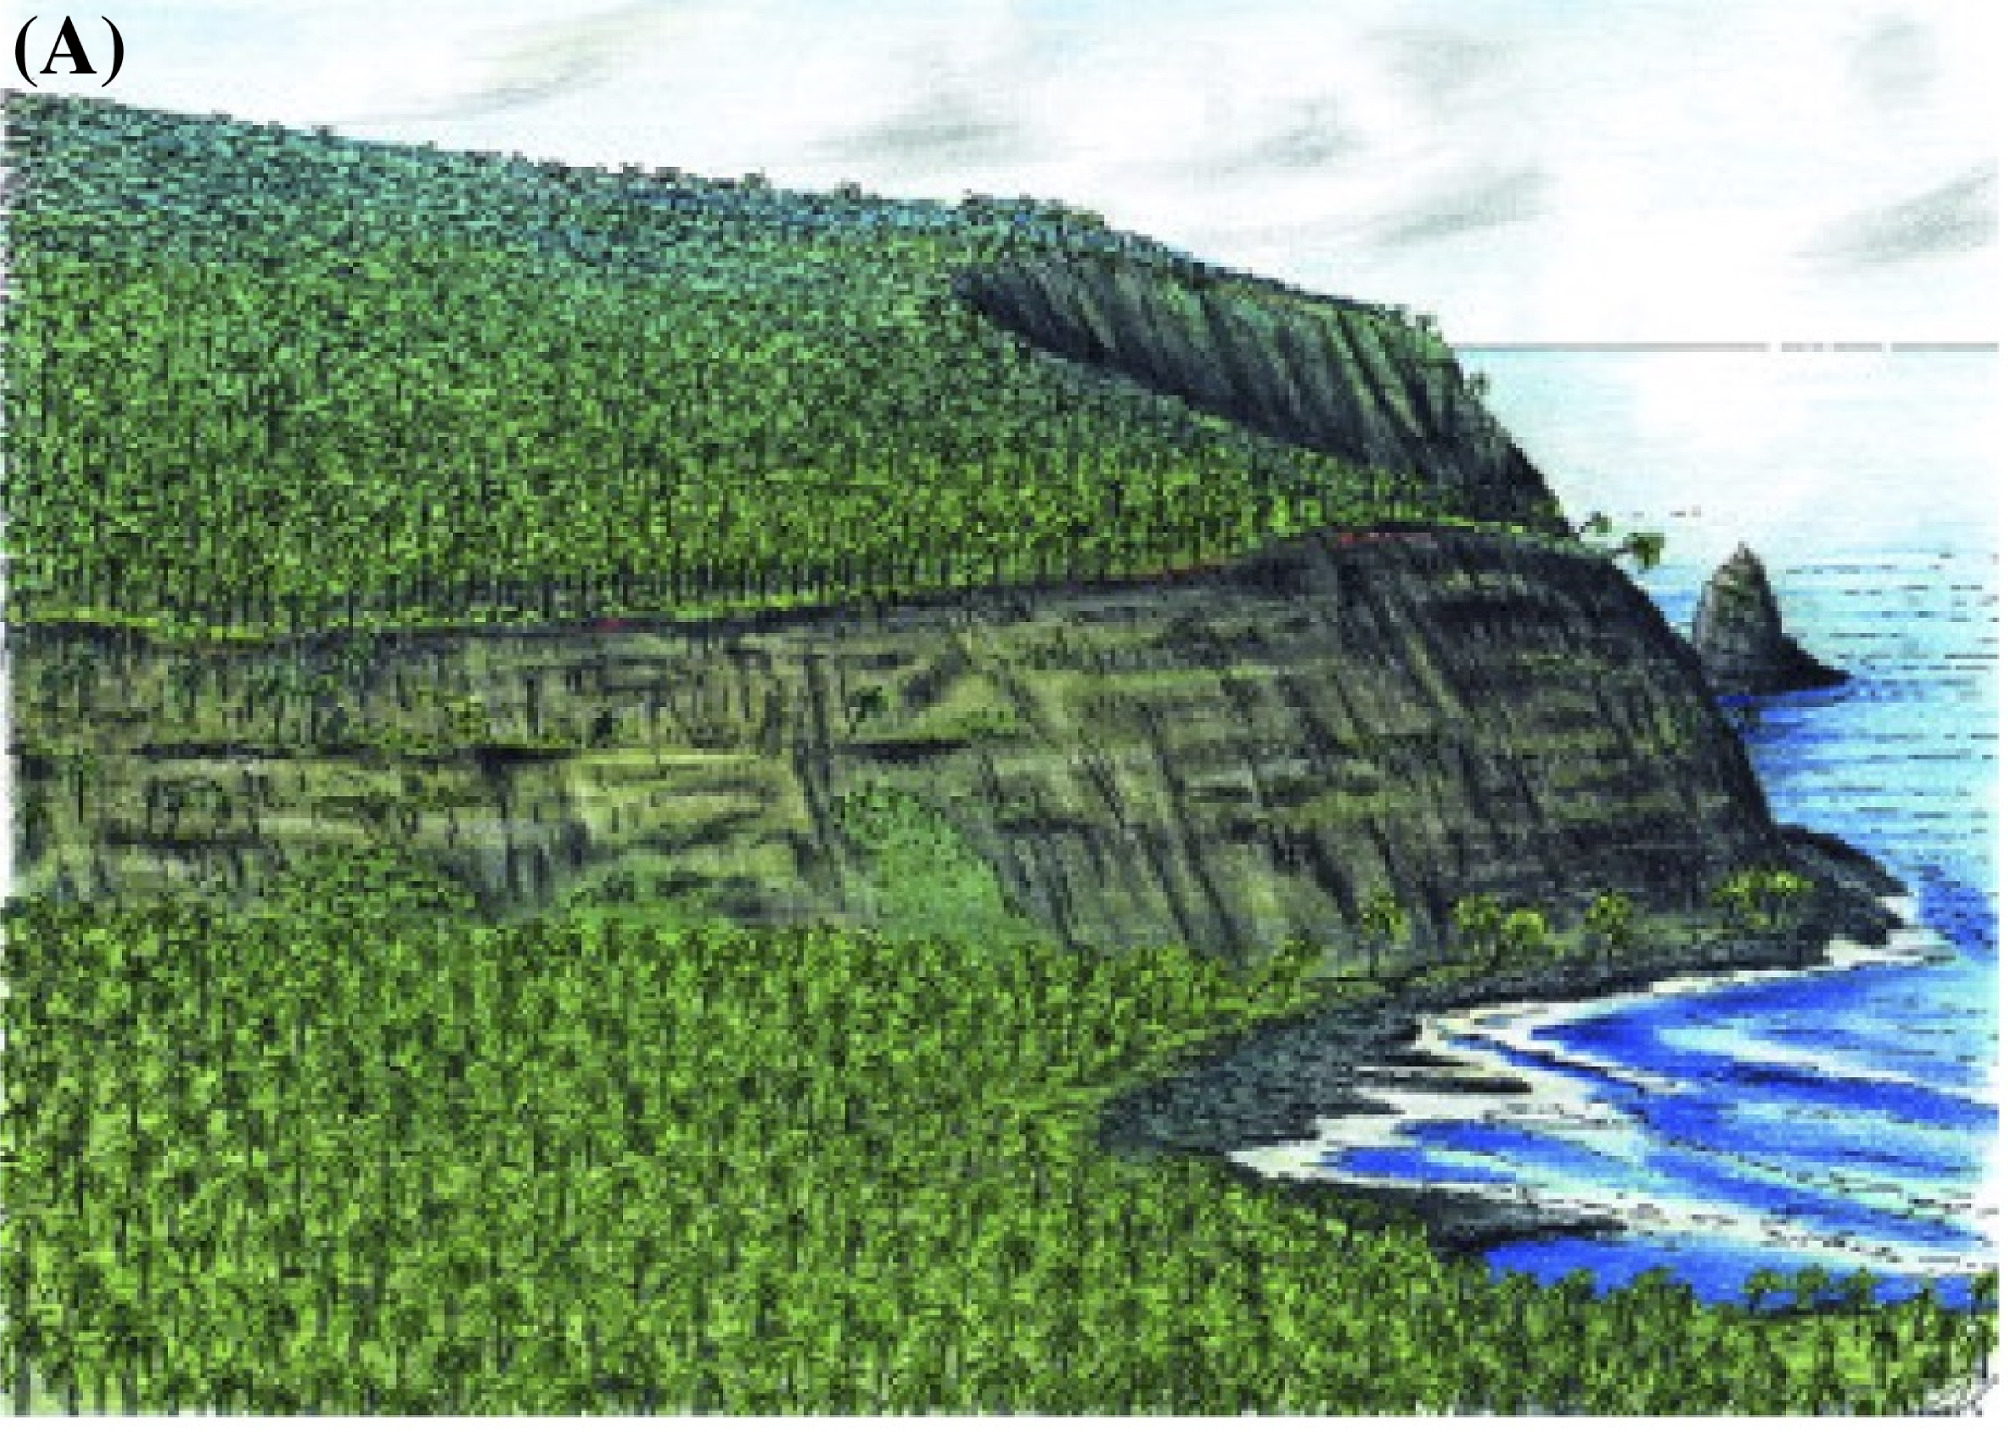
\includegraphics[height=4cm]{images/ForestGerdCloseRull2020.jpg}
	\caption{Palm Forest}
	\flushright{\tiny Artisitc Rendering, \citet{Rull2020}}
	}	
	\only<2>{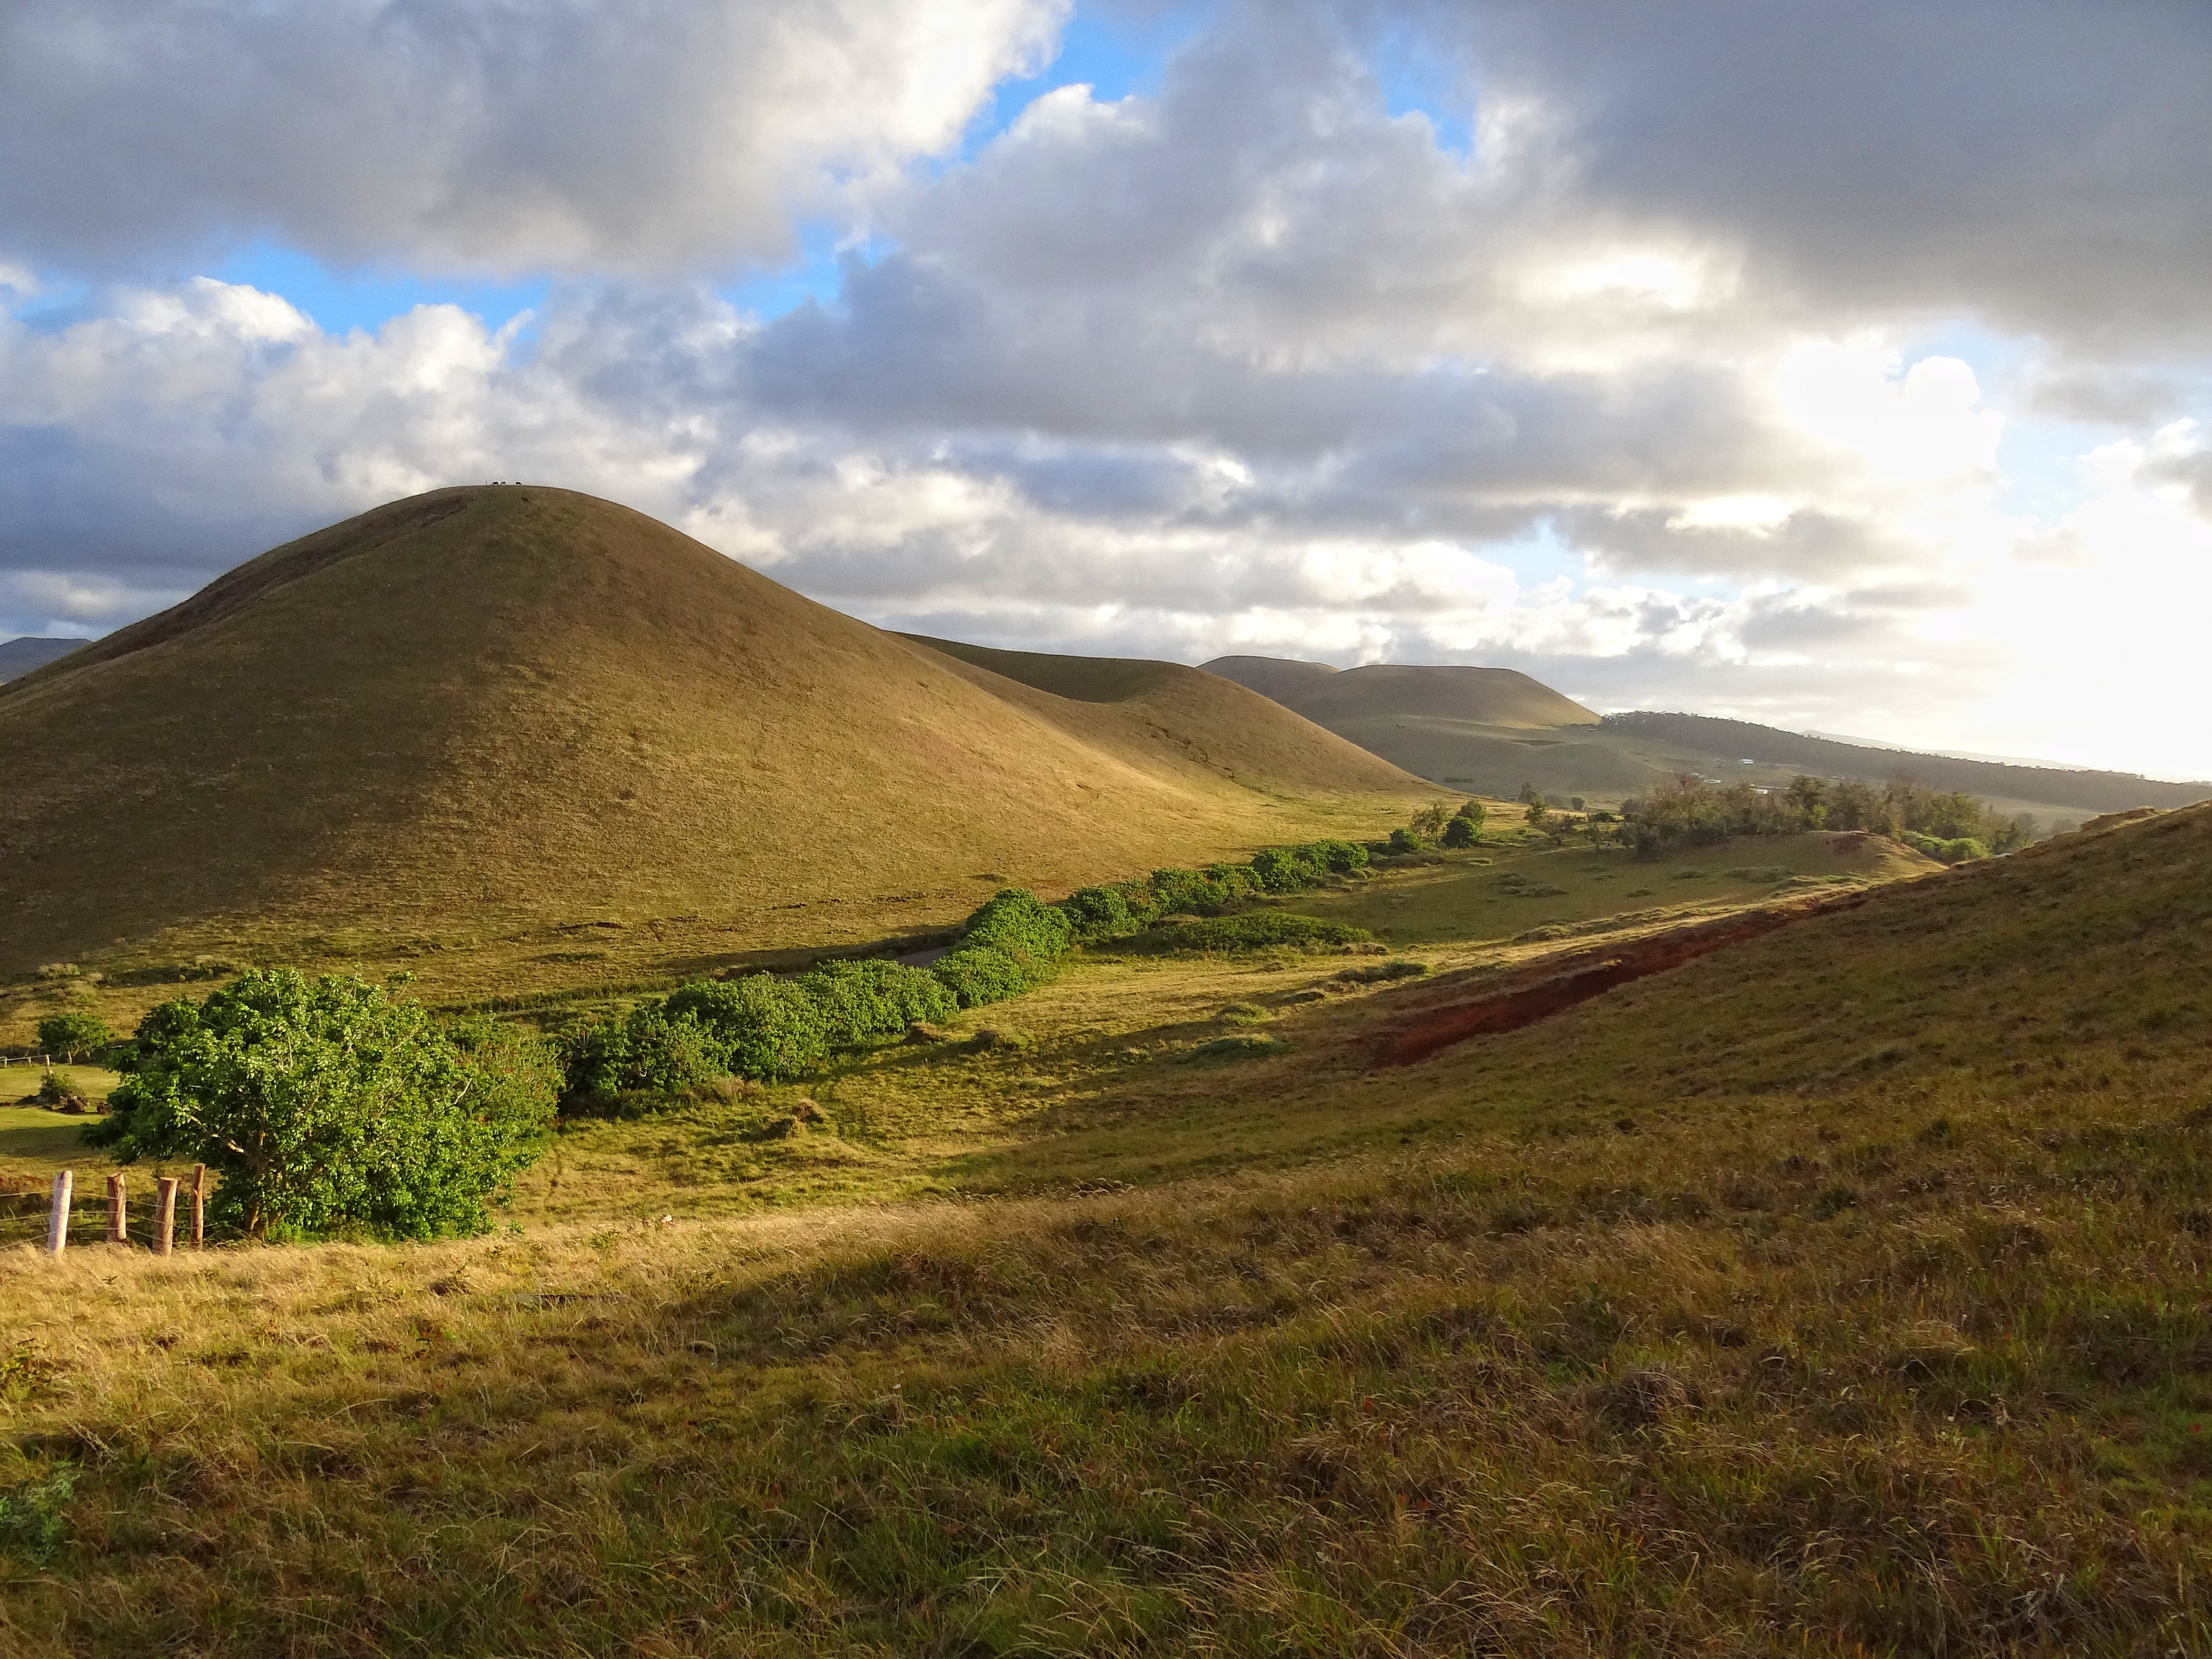
\includegraphics[height=4cm]{images/Rapa-Nui-Landscape.jpg}
	\caption{Deforestation}
	\flushright{\tiny Modern Day Image \url{en.wikipedia.org/wiki/Easter_Island}}
	}
	\only<3>{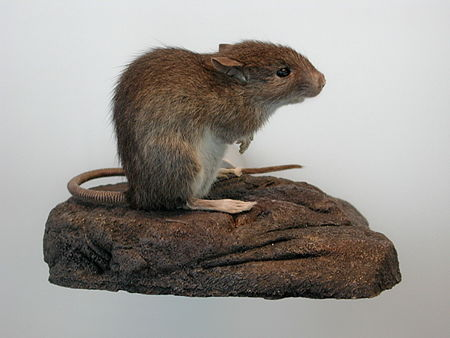
\includegraphics[height=4cm]{images/Pacific_rat.jpg}
	\caption{Pacfic Rats}
	\flushright{\tiny \url{de.wikipedia.org/wiki/Pazifische_Ratte}}
	}
	\only<4>{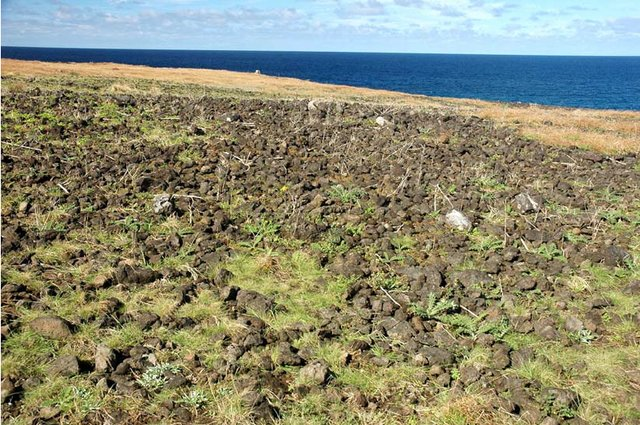
\includegraphics[height=4cm]{images/lithicMulching.jpg}
		\caption{Agriculture}
		 	\flushright{\tiny \citet{Hunt2009}}}
	\only<5>{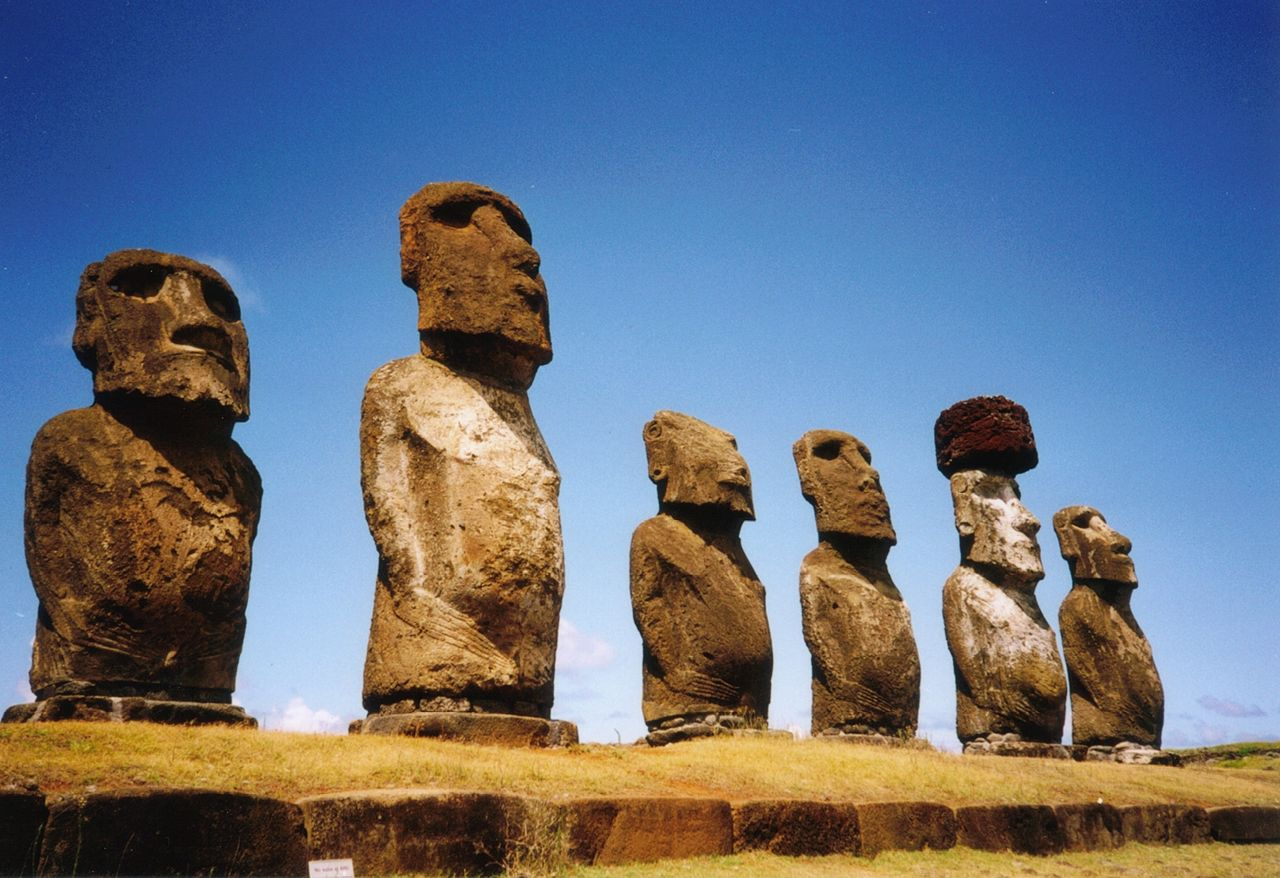
\includegraphics[height=4cm]{images/moai3.jpg}
		\caption{Moai Statues}
	\flushright{\tiny \url{https://nl.wikipedia.org/wiki/Moai}}
	}
	\only<6>{
		\begin{columns}
			\centering
			\begin{column}{0.4\textwidth}
				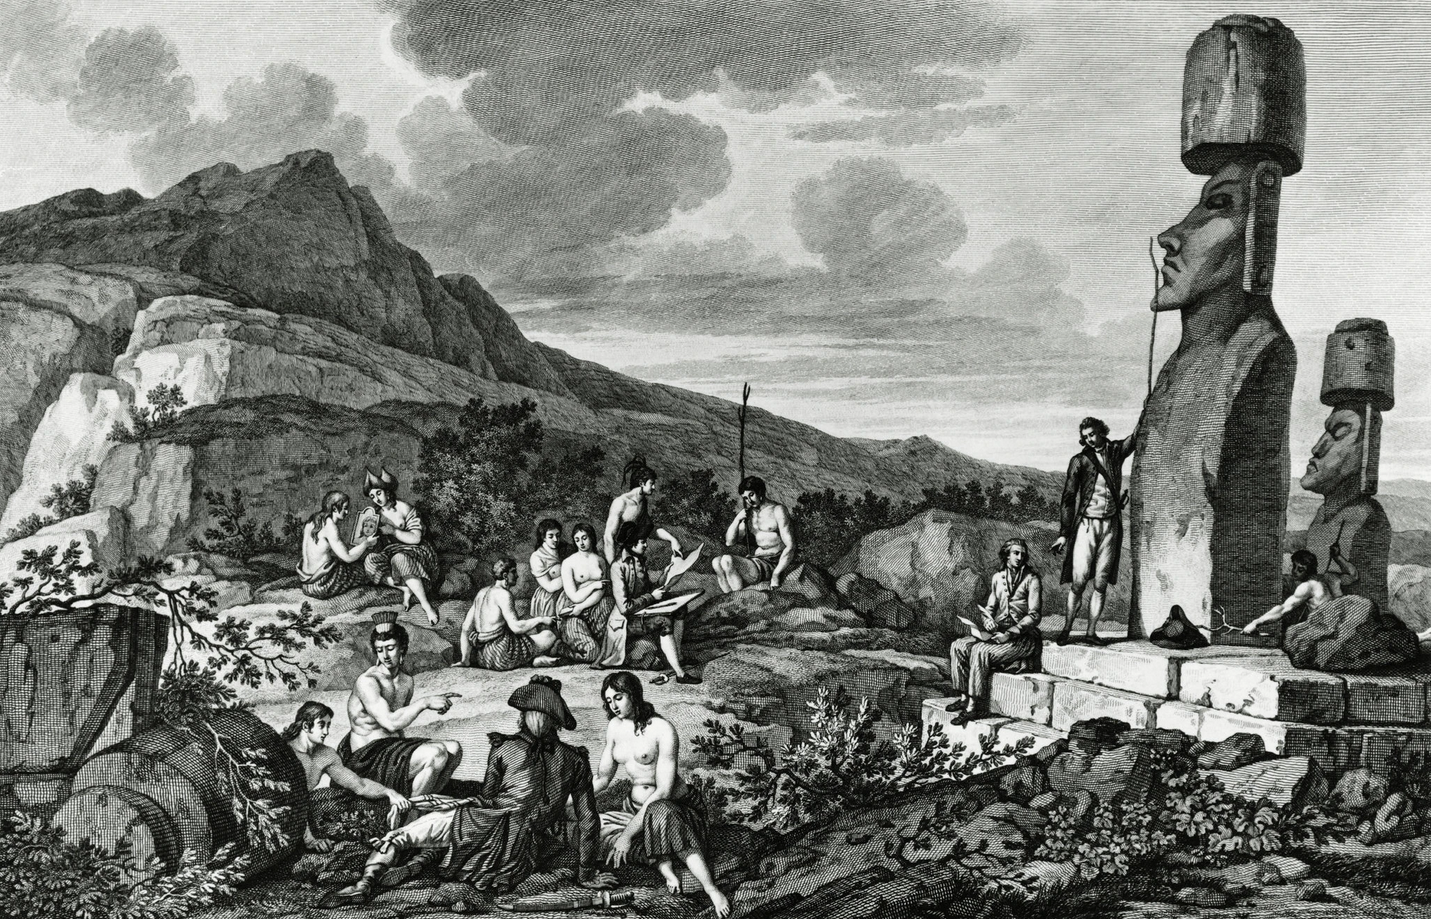
\includegraphics[height=4cm]{images/voyages.png}
				\caption{European Contact}
			\end{column}
			\begin{column}{0.4\textwidth}
			
				\textbf{Observations:} \vspace{0.2cm}
%				\begin{columns}
%					\begin{column}{0.3\textwidth}
%						\begin{itemize}
%							\item Advanced civilisation 
%							\item Initially Dense Forest
%						\end{itemize}
%					\end{column}
%					\begin{column}{0.1\textwidth}\centering
%						\textbf{\Huge \lightning}
%					\end{column}
%					\begin{column}{0.6\textwidth}
%						\begin{itemize}
%							\item Declining population number, 
%							\item Moai on the floor, 
%							\item Barren Island
%						\end{itemize}
%				\end{column}
%				\end{columns}
			\begin{itemize}
				\item Advanced civilisation 
				\item Initially dense forest
				\item Barren island
				\item Declining population number
				\item Moai lying on the ground
			\end{itemize}
			\end{column}
		\end{columns}
	\flushleft{\tiny  \url{www.nytimes.com/2017/10/12/science/easter-island-dna-south-america.html}}
	}

		
%	\only<7>{\centering \textbf{Observations}\begin{columns}
%			\begin{column}{0.4\textwidth}
%				\begin{itemize}
%					\item Dense Forest before human arrival
%					\item Built Moai Statues
%					\item Used Advanced farming techniques
%				\end{itemize}
%			\end{column}
%		\begin{column}{0.05\textwidth}
%			\centering
%			{\Huge\lightning}
%		\end{column}
%			\begin{column}{0.4\textwidth}
%				\begin{itemize}
%					\item Only a few thousand people ($100$ in $1860\, {\rm A.D.}$) 
%					\item Moai Statues on the floor
%					\item  Barren Island (no large vegetation)
%				\end{itemize}
%				
%			\end				\end{columns}{column}
%		\end{columns}}
\end{figure}
\begin{figure}
	\centering

\only<1-3>{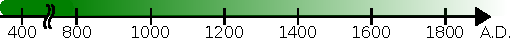
\includegraphics[width=0.6\linewidth]{images/timeline}}
\only<4,5>{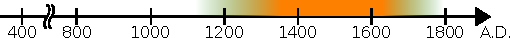
\includegraphics[width=0.6\linewidth]{images/timeline_agric}}	\only<6>{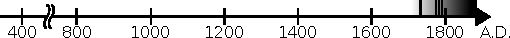
\includegraphics[width=0.6\linewidth]{images/timeline_european}}
\end{figure}
\end{frame}

\begin{frame}{The Mystery -- Two Major Narratives}
\begin{columns}
		\begin{column}{0.4\textwidth}
		\textbf{Ecocidal View}\\ \citet{Brander1998}, \citet{Diamond2011}, \citet{Bahn2017} \\ \ \\
		Early arrival, \\ 
		\ra Population grows slowly exponentially, \\
		\ra Intensification of agriculture and deforestation, \\
		\ra Population reaches $6k$ to $20k$ people in 17th century, \\ 
		\ra Overexploitation of resources and conflict (Malthusian catastrophe),
		\\
		\ra `Collapse' prior to European contact
	\end{column}


	\begin{column}{0.4\textwidth}
		\textbf{Genocidal View}\\ \citet{Peiser2005}, \citet{Hunt2007}, \citet{Basener2008}\\ \  \\
		Late arrival, \\
		\ra Population grows quickly and then remains constant at $4k$ people, \\
		\ \\
		\ra Rats cause deforestation, \\
		\ra Humans resilient, \\
		 \ \\
		\ra European contact triggers decline due to slave trades and diseases \\
		 \ \\
		 \ \\
		 

	\end{column}

\end{columns}
\centering
{\color{red}$\Downarrow$}\\
{\color{red} Population dynamics?}
\end{frame}


%
%\begin{frame}{The Mystery -- Two Narratives}
%\begin{columns}
%	\begin{column}{0.2\textwidth}
%		\ \\ \ \\ \ \\
%		\begin{itemize}
%			\item Arrival
%			\item Growth of Human Population
%			\item Deforestation
%			\item Agriculture intesification
%			\item Population size peak
%			\item Aftermath
%		\end{itemize}
%	\end{column}
%	\begin{column}{0.4\textwidth}
%		\textbf{Genocidal View}\\ \citet{Hunt2007} \\ \ 
%		\begin{itemize}
%			\item $1200\, {\rm A.D.}$
%			\item Fast 
%			\item Because rat population sky-rockets
%			\item immediately, after $1200\, {\rm A.D.}$
%			\item at $4$ k people in $14th century$
%			\item Civilisation resilient to environmental degradation, but `genocide' due to European diseases and slave trade
%		\end{itemize}
%	\end{column}
%	\begin{column}{0.4\textwidth}
%		\textbf{Ecocidal View}\\ \citet{Diamond2011}, \citet{Bahn2017}, \citet{Brander1998}
%		\begin{itemize}
%			\item before $1000\,{\rm A.D.}$
%			\item Slow
%			\item Humans started deforesting and lived off the natural resources (provided by trees)
%			\item only after $1200\, {\rm A.D.}$
%			\item at $6-20$ k people in $17$th century
%			\item Overexploitation and erosion, resources scarce, potential conflict, `collapse' (Malthusian Catastrophe) prior to European contact
%		\end{itemize}
%	\end{column}
%\end{columns}
%\end{frame}


\section{Traditional Approach: Dynamic System Modelling}
% !TEX root = presentation_29Jun.tex

\begin{frame}{Mathematical Modelling of Human-Resource Interaction}

\begin{itemize}
	\item Macroscopic variables: 
	\begin{itemize}
		\item Resource stock (palm trees): $T$
		\item Human population size: $P$
	\end{itemize} 
	\ra Human-resource interactions (Lotka-Voltera predator-prey type)
	\item So far: Dynamics described by ordinary differential equations (ODEs)
	\begin{eqnarray*}\label{eq:ode}
		\frac{d \text{P}}{dt} & = & r_\text{P} (\text{T, P, H}(\text{P})) \ \cdot \ \text{P} \\
		\frac{d \text{T}}{dt} & = & r_\text{T} (\text{T}) \ \cdot \ \text{T} \ - \   \text{H}(\text{P}) 
	\end{eqnarray*}	
with \center{$\text{H}(\text{P})$ = harvest of population $\text{P}$; \\$r_{\rm T,P}$ = functions for rates of growth}
\end{itemize}
\end{frame}

\begin{frame}{The first model on Easter Island: \citet{Brander1998}}
%The first Model: \citeTitle{Brander1998}
\centering

%\item Population grows/decays exponentially. Consumption of the resource increases the rate
%\item Result: Slow regrowth of the palm tree vs.\ faster exponential population growth \ra Malthusian Catastrophe (a.k.a.\ `Boom-Bust')

\begin{columns} \begin{column}{0.7\textwidth}
		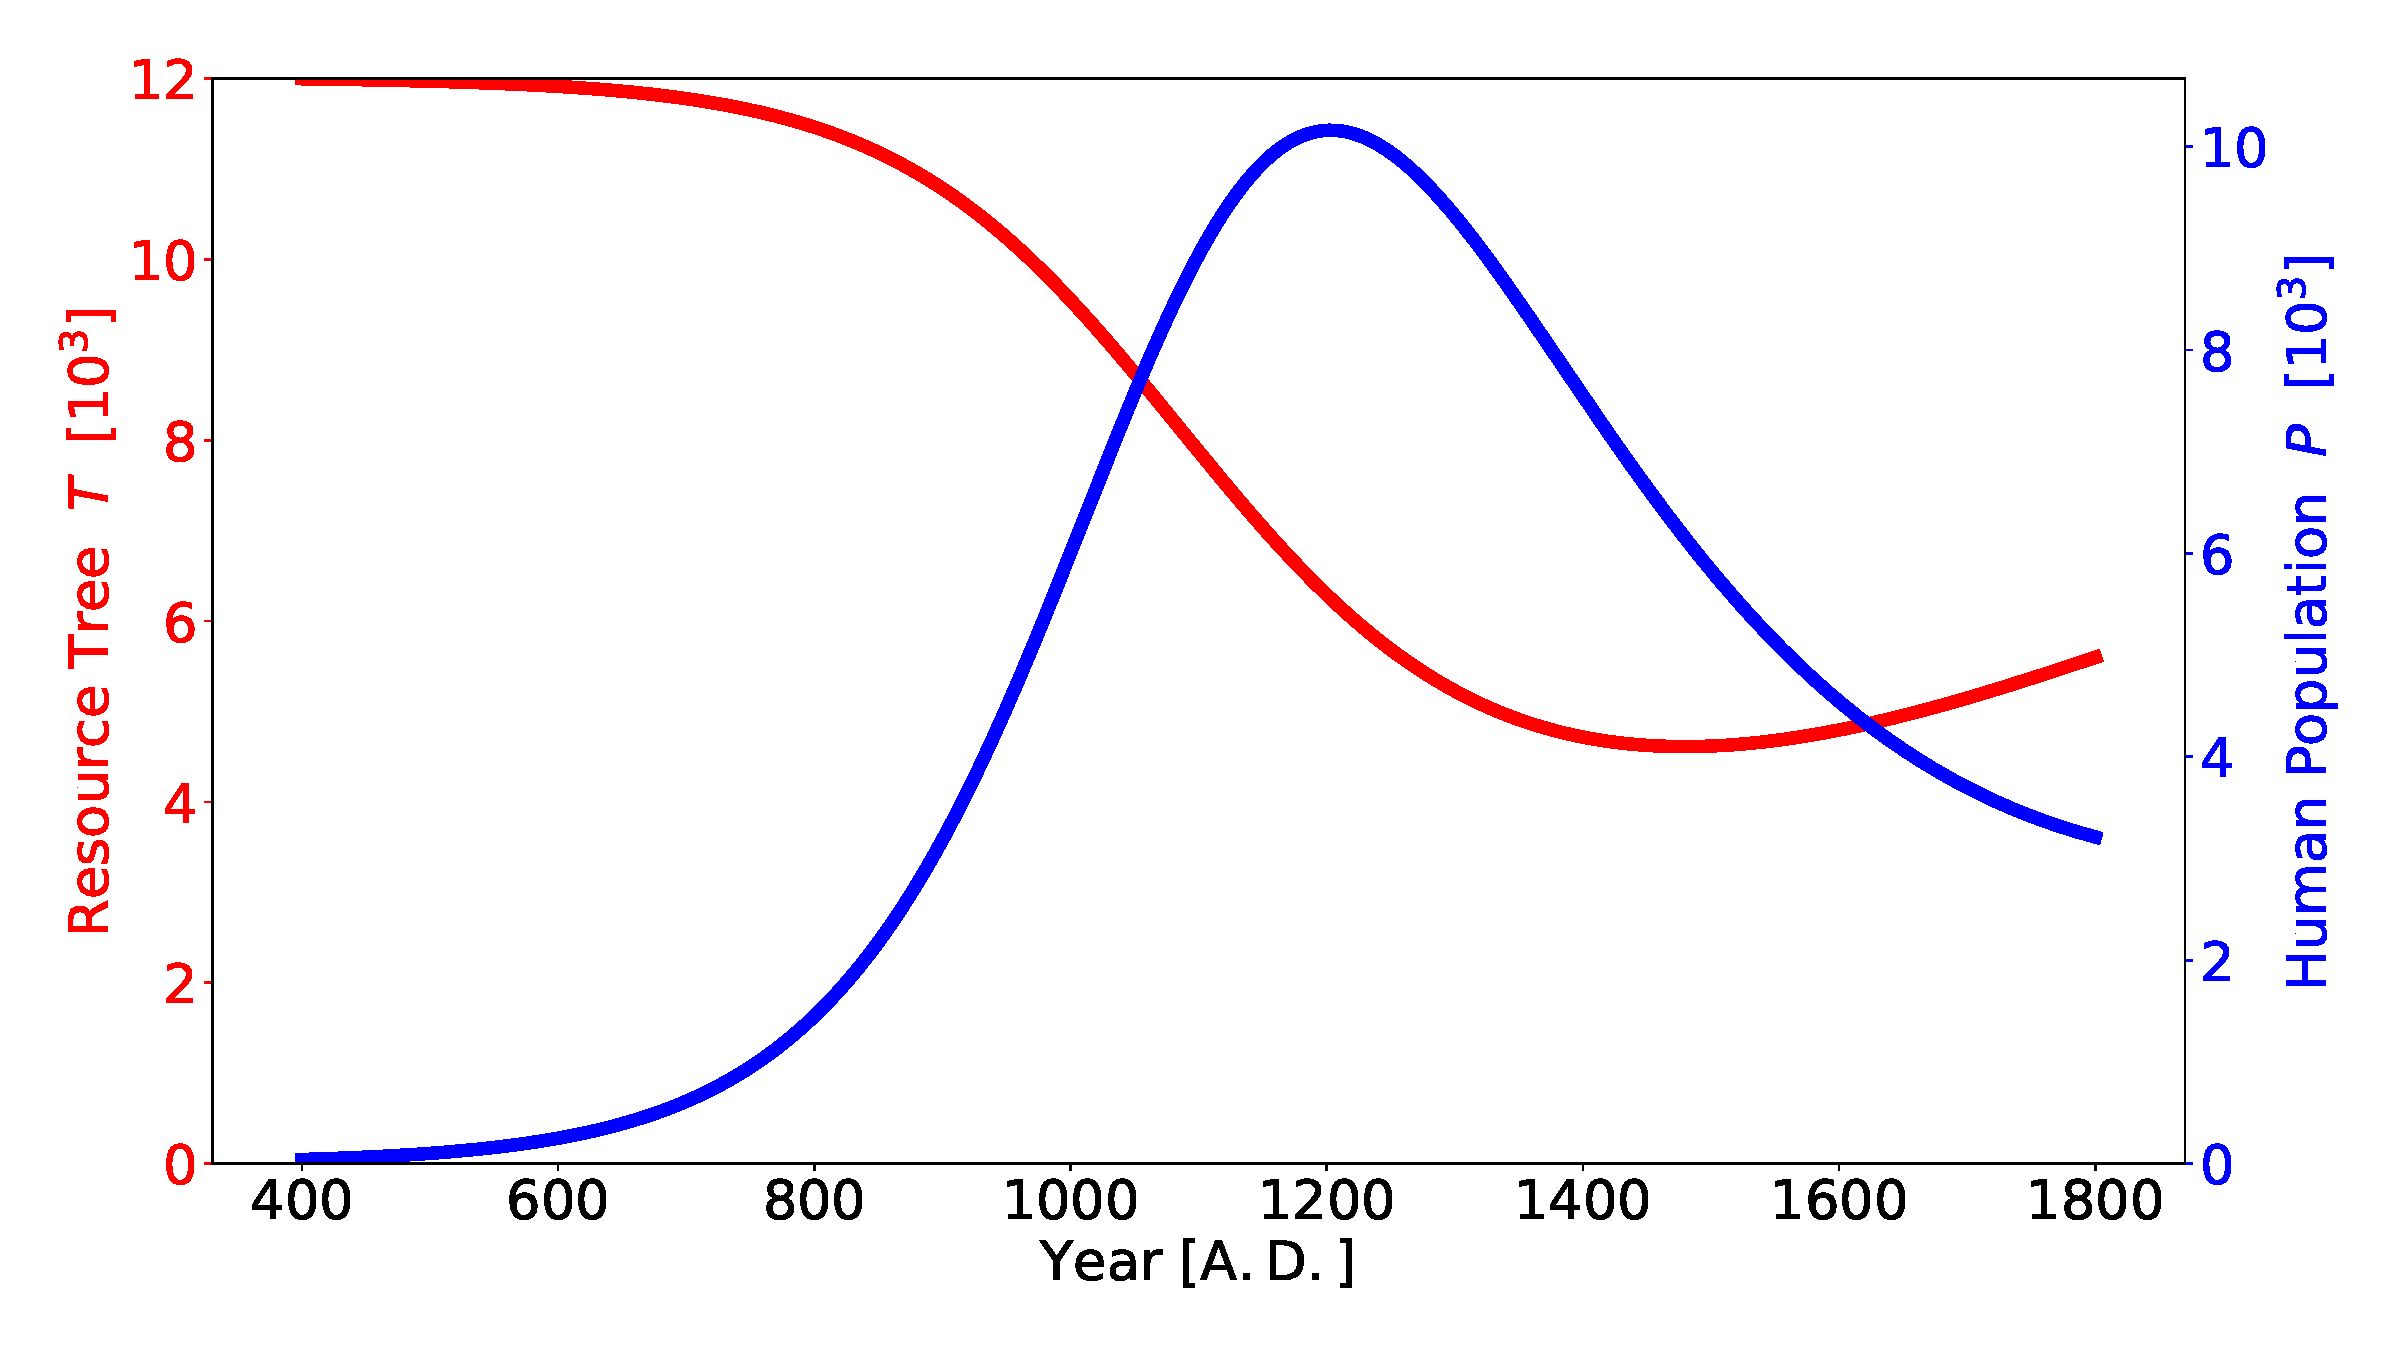
\includegraphics[width=\textwidth]{../../Thesis/images/Brander1998_EIBaseCase_presentation} 
\end{column}
\begin{column}{0.2\textwidth}
	{\footnotesize Model by \citet{Brander1998}}
\end{column}
\end{columns}
	

\begin{itemize}
\pause\item Extensions:
\begin{itemize}
	\item Socio-economic institutions \citep{Good2006}
	\item Second resource \citep{DAlessandro2007}
	\item Rat population \citep{Basener2008}
	%\item 1-dim spatial component \citep{Basener2011}
	\item Disease model \citep{Brandt2015}
\end{itemize} 
\end{itemize}                                                       
\end{frame}

\begin{frame}{Shortcomings of Dynamic System Models}
\begin{itemize}
\item Uncertainty in Parameters\\ \vspace{0.3cm}
{\centering 
	\begin{columns}
		\begin{column}{0.7\textwidth}
			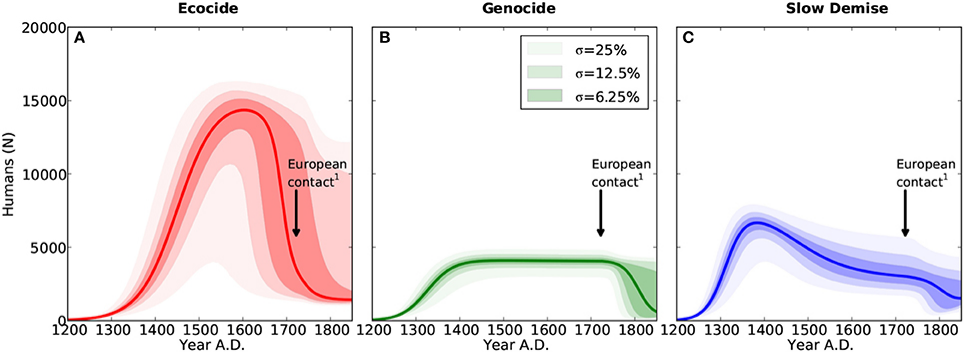
\includegraphics[width=\textwidth]{images/Brandt2015_onlyHumans}
		\end{column}
		\begin{column}{0.15\textwidth}
			{\footnotesize Model by \citet{Brandt2015}}
		\end{column}
	\end{columns}
} \vspace{0.3cm}
\ra Macroscopic view does not give insight into plausibility of resulting trajectory
\pause\item Neglect ...
\begin{itemize}
\item Spatial constraints
\item Irreducibility and heterogeneity
\item Adaptation and emergent phenomena
\item Stochasticity
\end{itemize} 
\vfill 
{\tiny More in e.g.\ \citet{Bookstaber2019}, \citet{Bonabeau2002}}
\end{itemize}
\end{frame}



\section{New Approach: Agent-Based Modelling (ABM)}
% !TEX root = presentation_29Jun.tex

%\begin{frame}{Agent Based Modelling}
%\end{frame}
%
%\begin{frame}{Modelling Societies with ABM}
%
%%\begin{block}{\citet{Bookstaber2019}}
%%	\TODO
%%\end{block}
%\end{frame}


\begin{frame}{What is Agent-Based Modeling (ABM)}
%\begin{itemize}
%	\item Discrete units (Agents) in an environment with specific traits
%	\item Asynchronous and autonomous update of agents:
%	%\item In each update: 
%	\begin{itemize}
%		\item interaction based on rules and heuristics \\(often non-linear, heterogeneous, stochastic, adaptive, path-dependent)
%		\item autonomous decisions of agents
%	\end{itemize}
%	\item Aggregate variables are (1) outcomes of and (2) contexts for the agents decisions and actions \citep{Kohler2000}
%\end{itemize}



\begin{algorithm}[H]
	\textbf{Initialise} Environment  \\
	\textbf{Initialise} discrete Agents with specific traits in some location within the environment\\
	\For{$t \ \in\  \{t_{\rm start}, t_{\rm end}\}$}{
		\For{agent (in asynchronous order)}{
			\textbf{Interaction} between agent and environment based on rules and heuristics\\
			\textbf{Update} agent according to autonomous decisions
		}
		\textbf{Calculate} aggregate variables of environment and agents
	}
	\caption{General Structure}
\end{algorithm}
\end{frame}



\begin{frame}{Advantages of ABM with respect to ODE models}


% 	\begin{block}{\citet{Epstein1996}}%, as cited in \citet{Bonabeau2002}}
% 		 \begin{framed}
%	On Agent-Based Modelling:
%	"Perhaps one day people will interpret the question, ‘Can you explain [an observed social phenomenon]?’ as asking `Can you grow it?’"
%\end{framed}
%	 	\end{block}
 	 	%, as cited in \citet{Bonabeau2002}}
 	 	\begin{framed}
 	 		 \citet{Epstein1996}, \citet{Bonabeau2002} on Agent-Based Modelling:
 			\begin{center}
 				\textit{"Perhaps one day people will interpret the question, ‘Can you explain [an observed social phenomenon]?’ as asking `Can you grow it?’"
} 			\end{center}
 		\end{framed}

	From macroscopic, top-down description \ra to microscopic, bottom-up description
	\begin{enumerate}
		\item ABM allows for rules and heuristics to be 
		\begin{itemize}
			\item non-linear, discontinuous
			\item heterogeneous,
			\item stochastic, 
			\item adaptive \newline
			%\item path-dependent 
			\ra non-ergodicity \& computational irreducibility
		\end{itemize}
		\pause\item \ra Emergent phenomena
		%\item Non Ergodicity
		%\pause\item \ra Computational irreducibility
		\pause\item Decisions include stochasticity
		\pause\item Natural implementation of heterogeneous space dependency
	\end{enumerate}
\end{frame}


%\begin{frame}{Application of ABMs}
%\begin{itemize}
%	\item Typically: Problems related to cognitive psychology, game theory, and complexity science \citep{Bousquet2004}
%	\item Also, Socio-ecological Systems \citep{Muller-Hansen2017} \ra Human-Resource Interaction
%	\begin{itemize}
%		\item \ldots
%		\item Collapse of Ancient Societies
%		\begin{itemize}
%			\item Anasazi in Arizona, US \citet{Axtell2002}
%			\item Maya \citet{Heckbert2013}
%			\item Now: Easter Island
%		\end{itemize}
%	\end{itemize}
%\end{itemize}
%\end{frame}



\section{The Easter Island ABM}
% !TEX root = presentation_29Jun.tex


\begin{frame}{Easter Island ABM -- Overview}  
%\begin{overlayarea}{\textwidth}{\textheight} 
\begin{itemize}
	\item<2-> Agents (dots) are households of a few dozen (ca.\ up to $40$) individuals.
	\item<3-> Environment provides trees and farming products
	\item<3-> Agents harvest from local environment (cut trees and occupy farming sites)
	\item<4-> If successful, the agent's population grows (eventually producing more agents) \newline If not successful, it decreases and the agent moves
	\item<5-> Agents adapt their resource preference according to the perceived local environment
\end{itemize}%
	\centering
	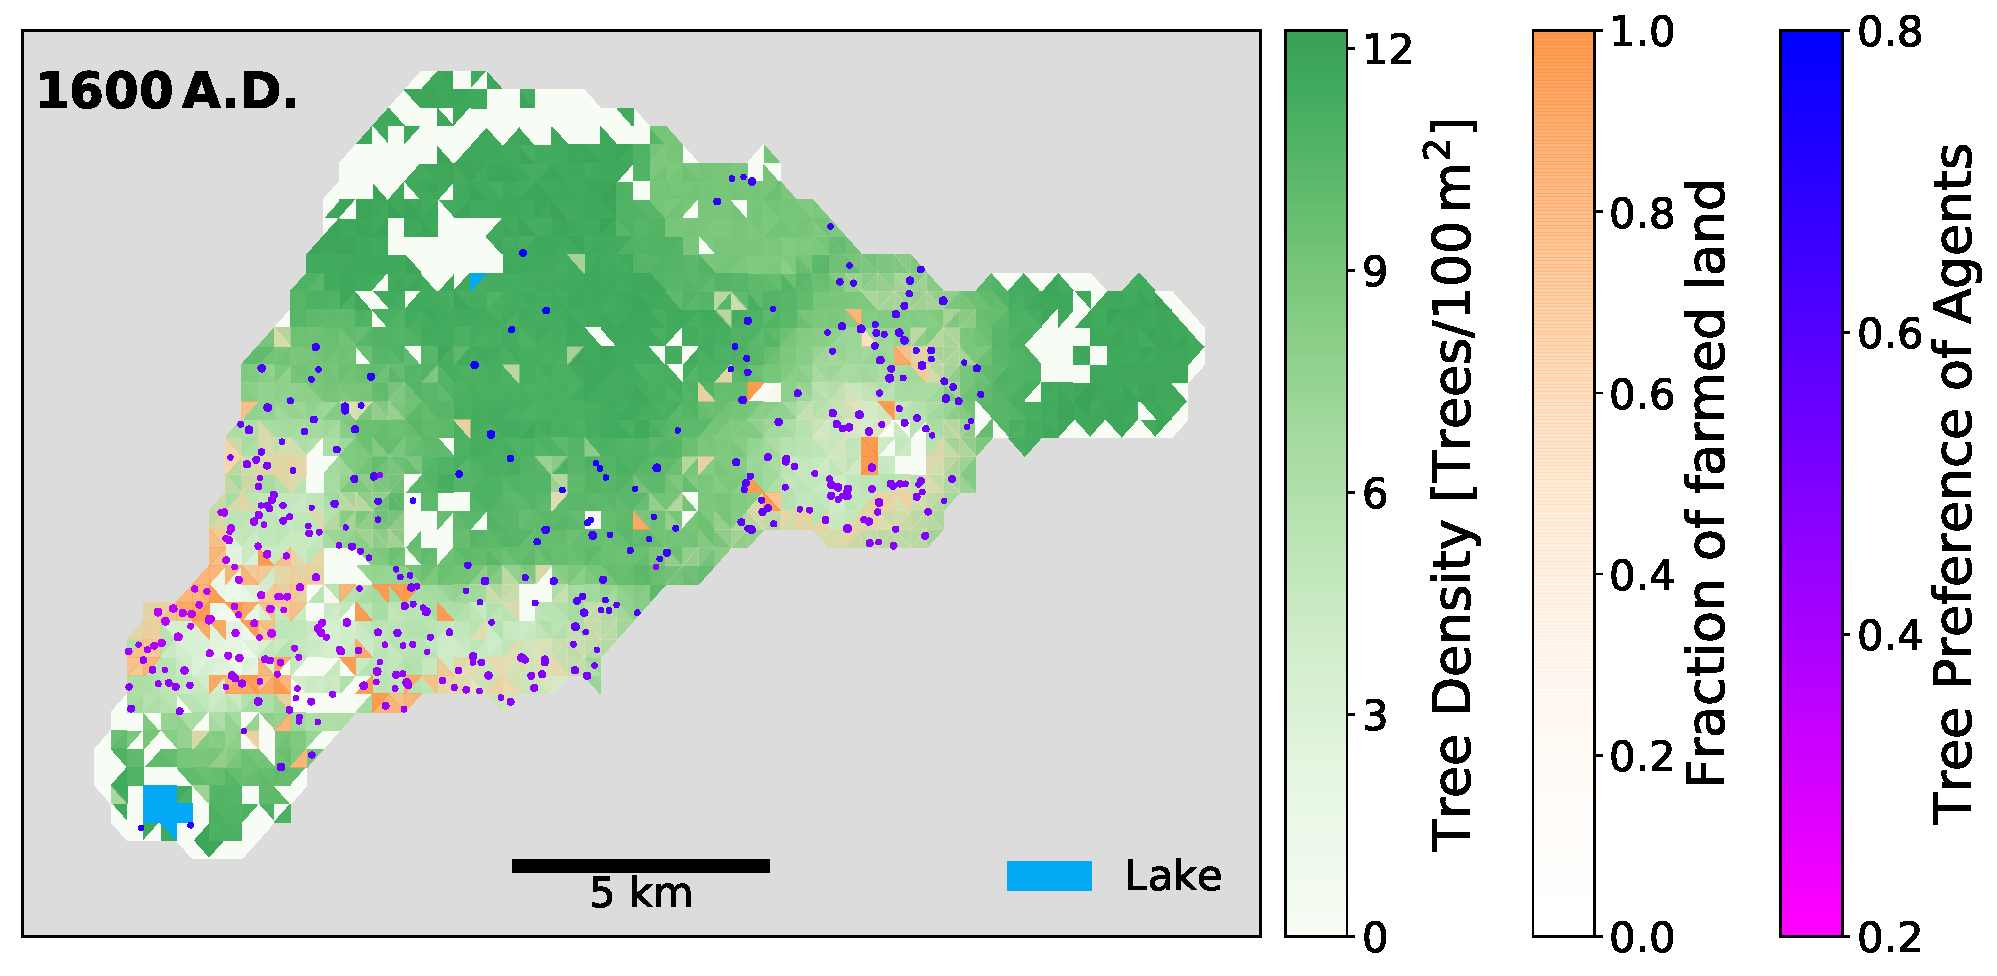
\includegraphics[width=0.7\linewidth]{images/map_time1600}
	%\captionof{figure}{Example Snapshot}
%\end{overlayarea}
\end{frame}

\begin{frame}{Create the Environment -- Discretisation}
	\centering
	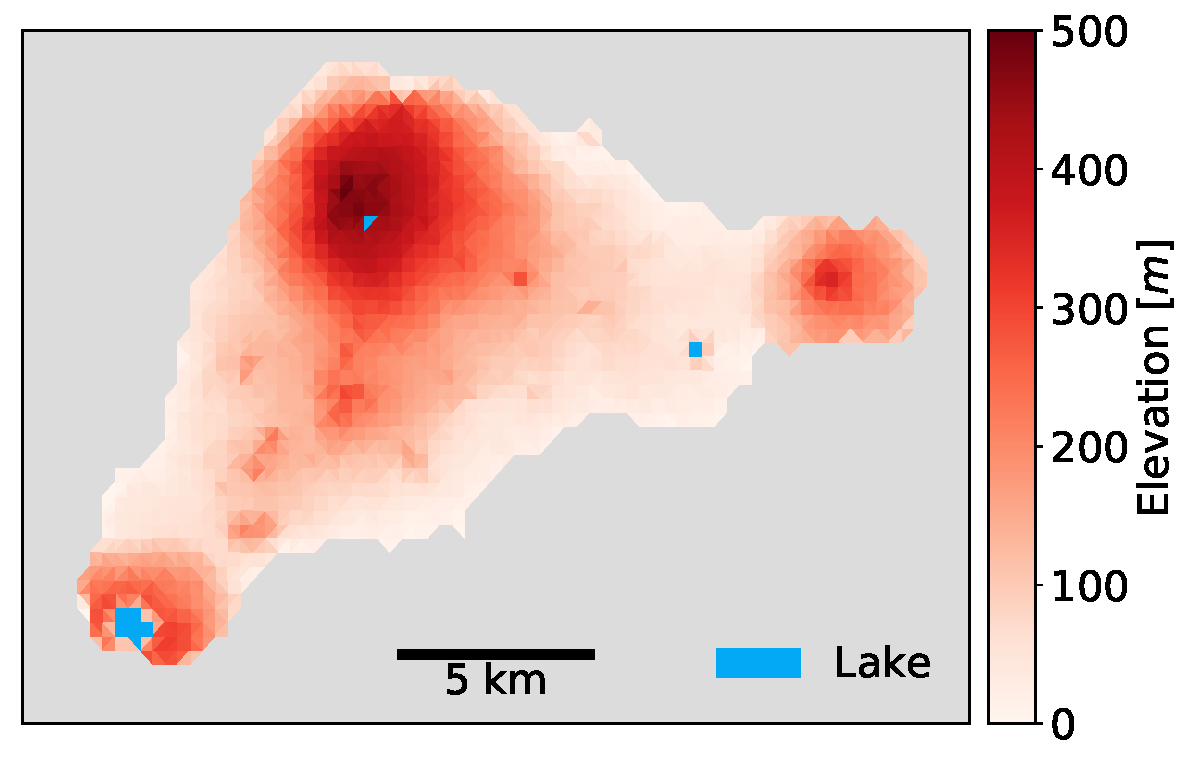
\includegraphics[width=0.7\linewidth]{Plot_elevation}


\end{frame}

\begin{frame}{Create the Environment -- Features}
\centering
\only<1>{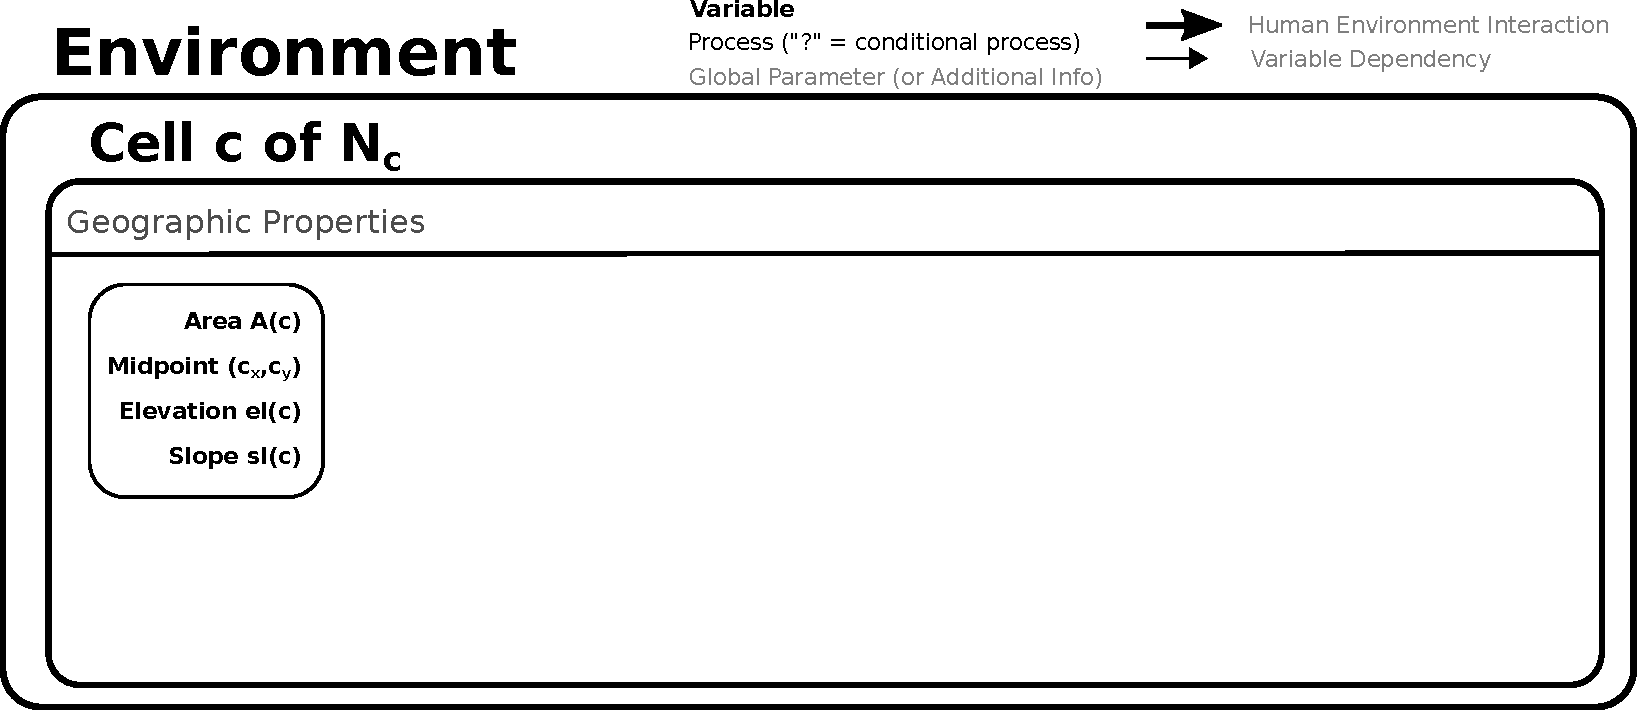
\includegraphics[width=0.7\linewidth]{SketchABM2/EnvironmentSketch_1}}
\only<2>{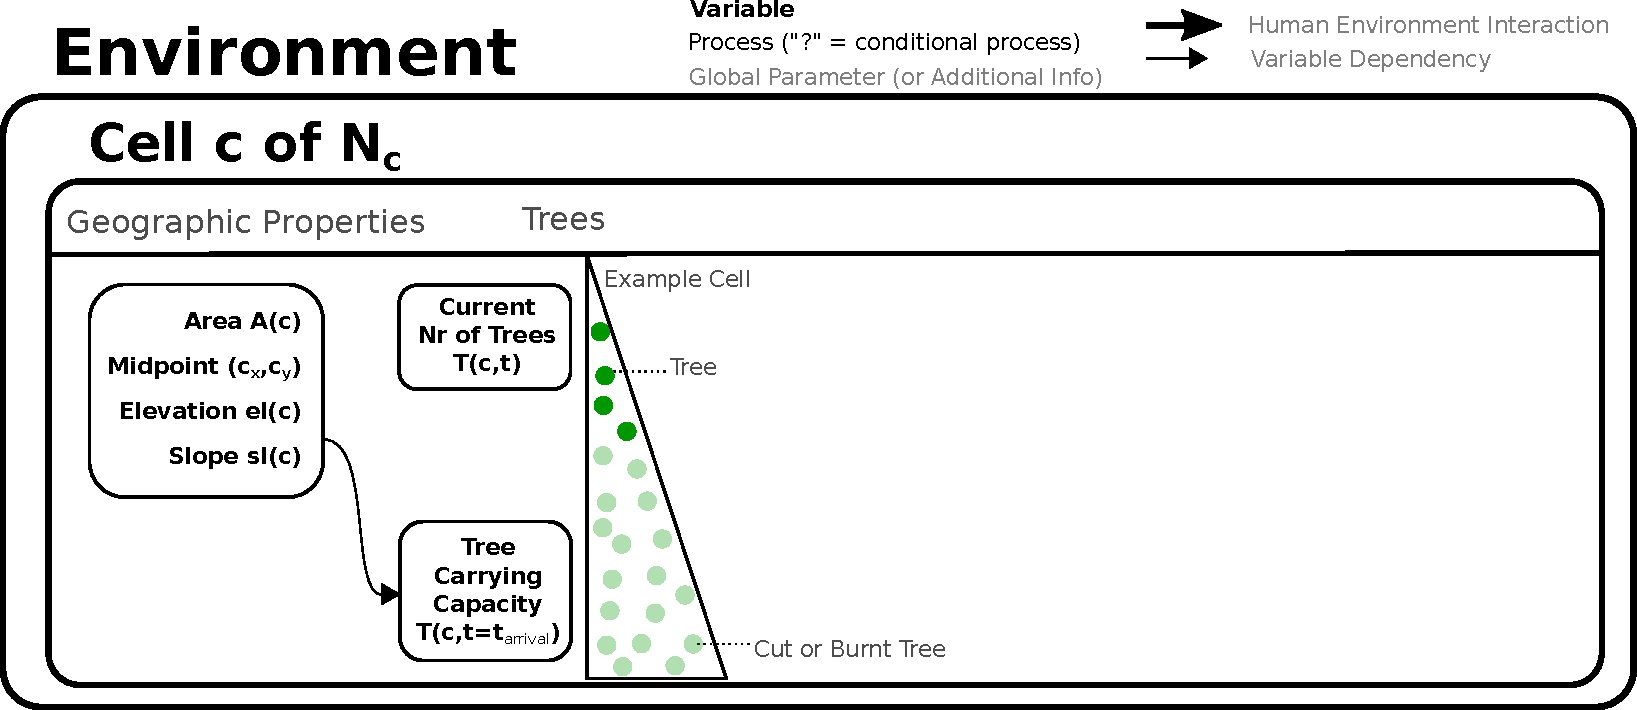
\includegraphics[width=0.7\linewidth]{SketchABM2/EnvironmentSketch_2}}
\only<3>{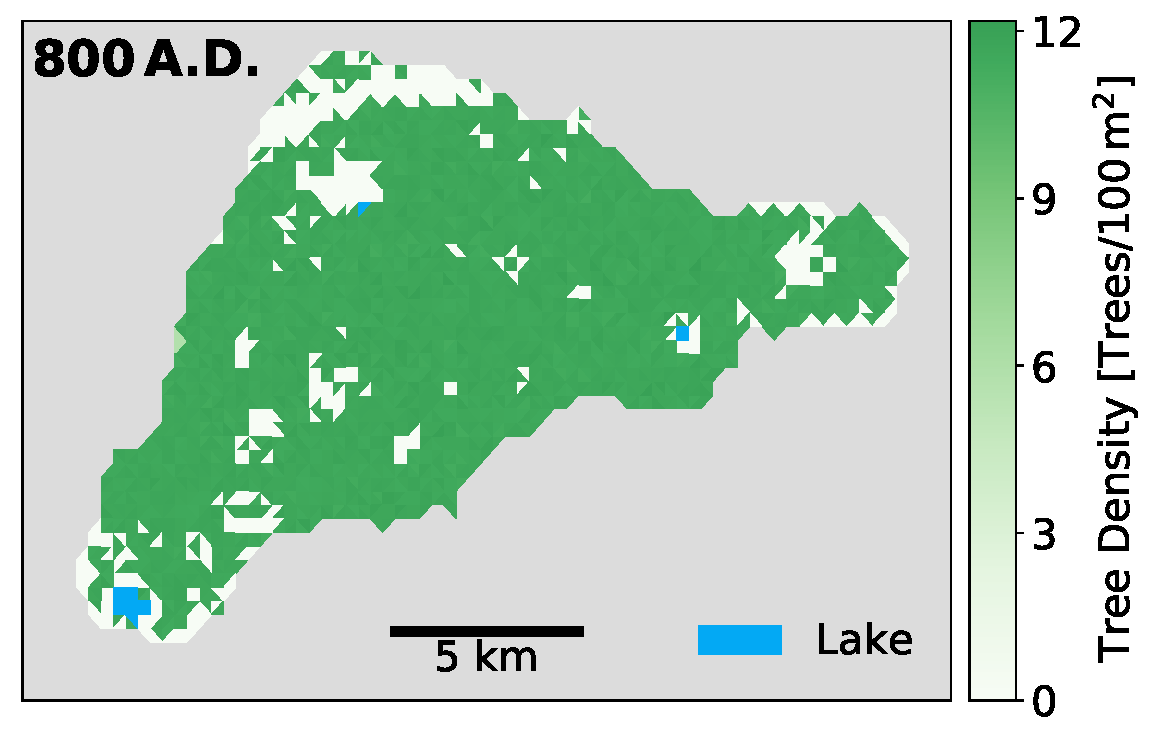
\includegraphics[width=0.7\linewidth]{map_carrCap}
\captionof{figure}{Based on \citet{Mieth2015}, \citet{Bahn2017}, \citet{Rull2020}}
}
\only<4>{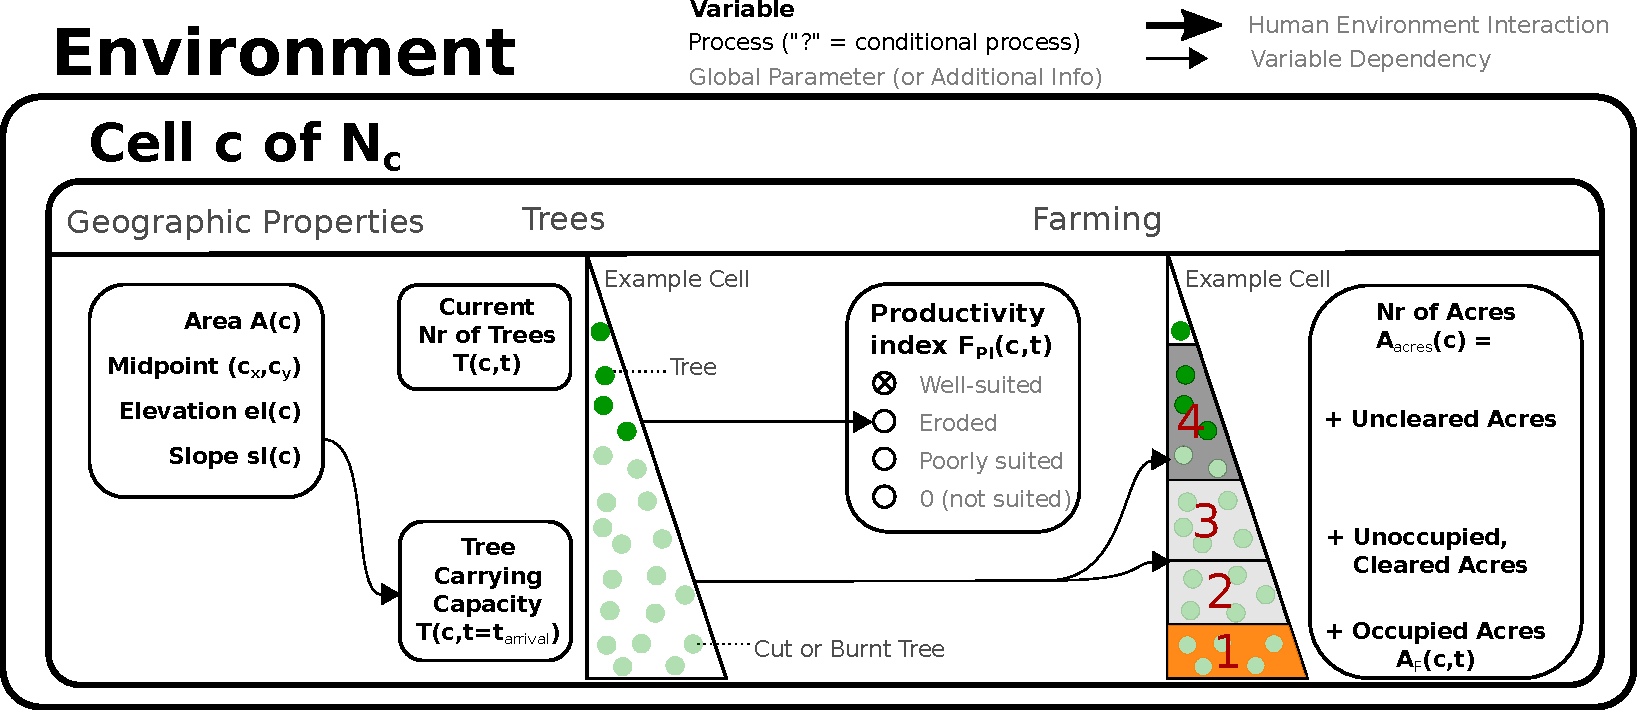
\includegraphics[width=0.7\linewidth]{SketchABM2/EnvironmentSketch_final}
	\captionof{figure}{$1\, {\rm acre} \ \hat{\approx} \ 100\, {\rm m} \, \times 40\,{\rm m}$.}}
\only<5>{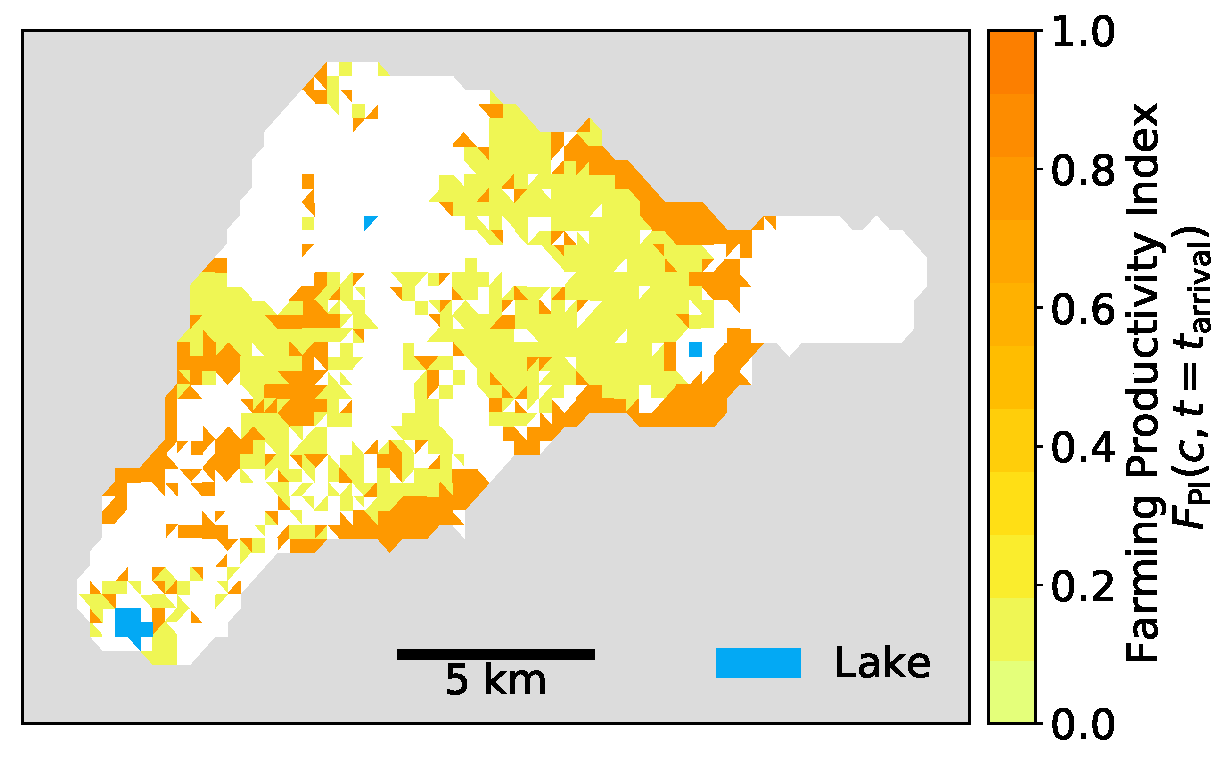
\includegraphics[width=0.7\linewidth]{Plot_F_PI_c}
	\captionof{figure}{Based on \citet{Louwagie2006}, \citet{Puleston2017}}}
\end{frame}

\begin{frame}{Agents and Interaction with Environment}
\centering
\only<1>{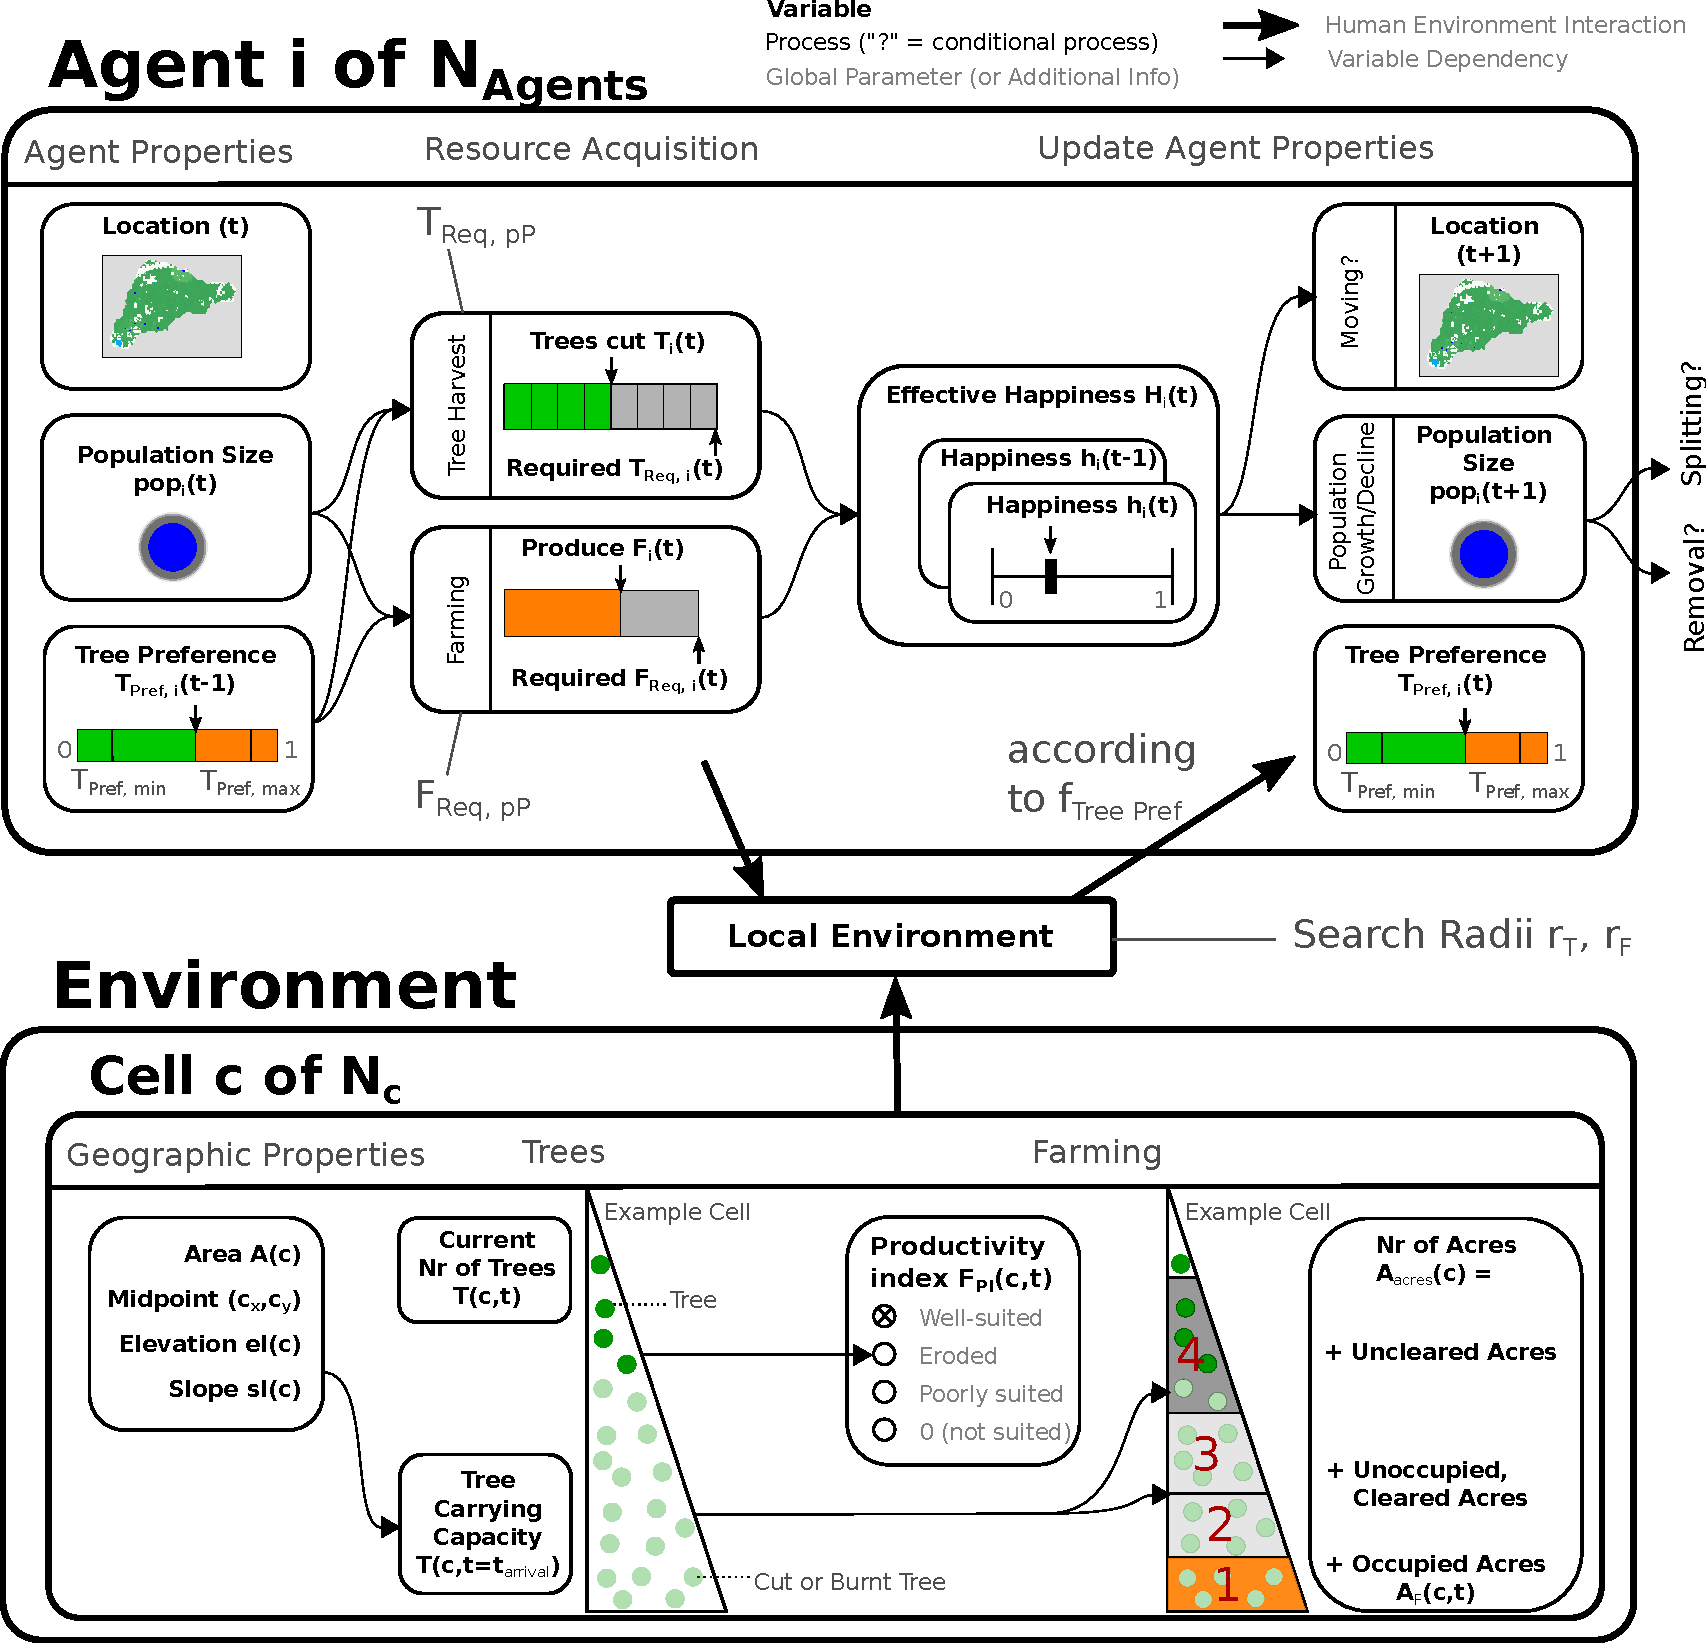
\includegraphics[width=0.55\linewidth]{SketchABM2/sketch_triangles}}
%\only<2>{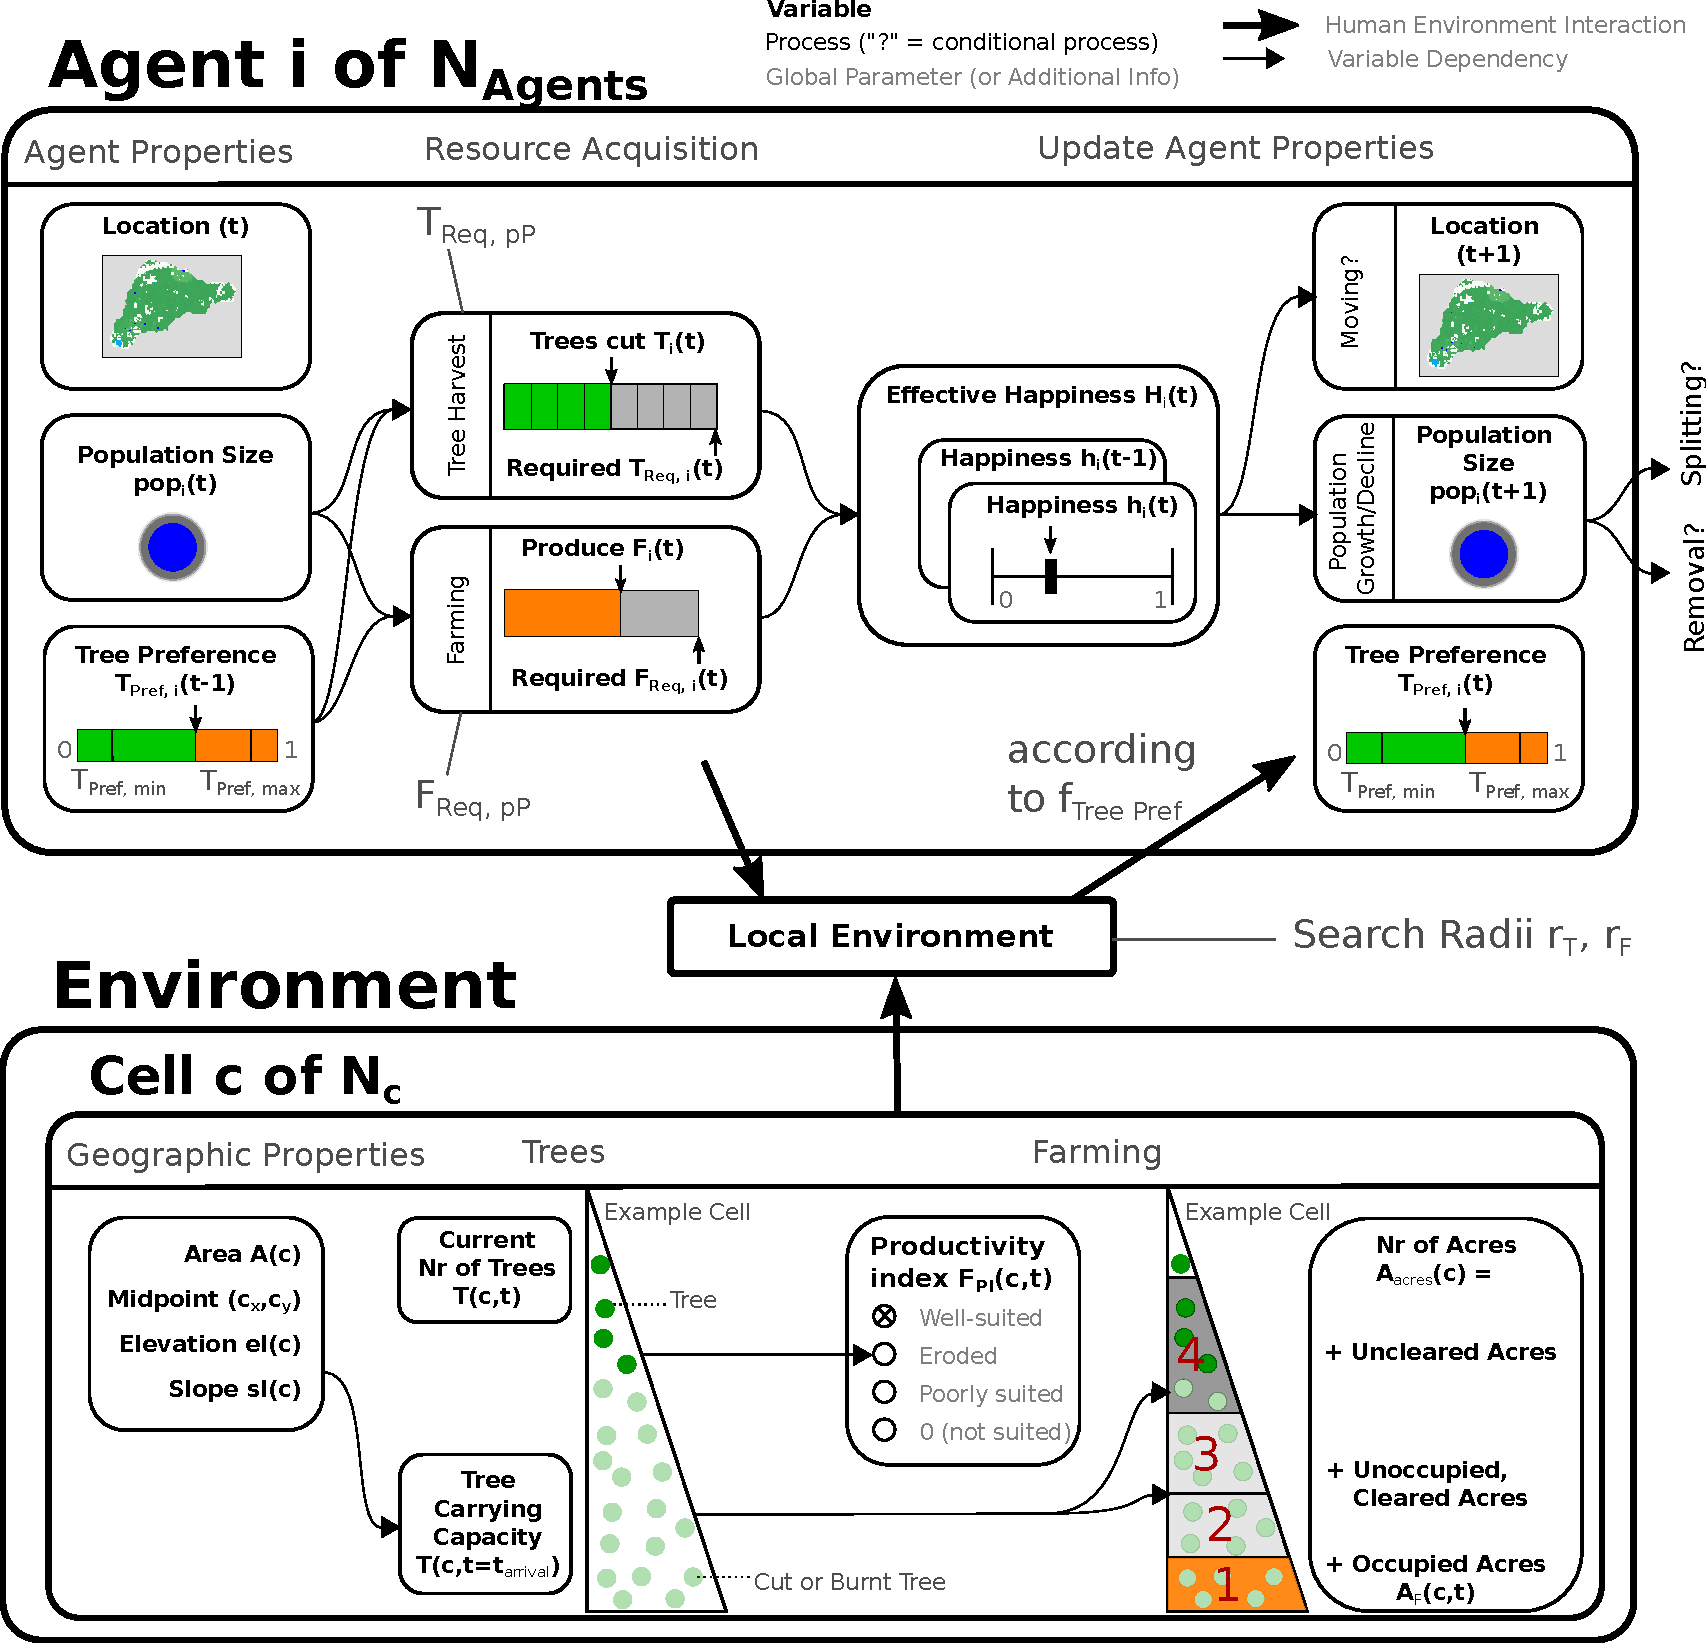
\includegraphics[width=0.85\linewidth]{SketchABM2/sketch_triangles}}
\only<2>{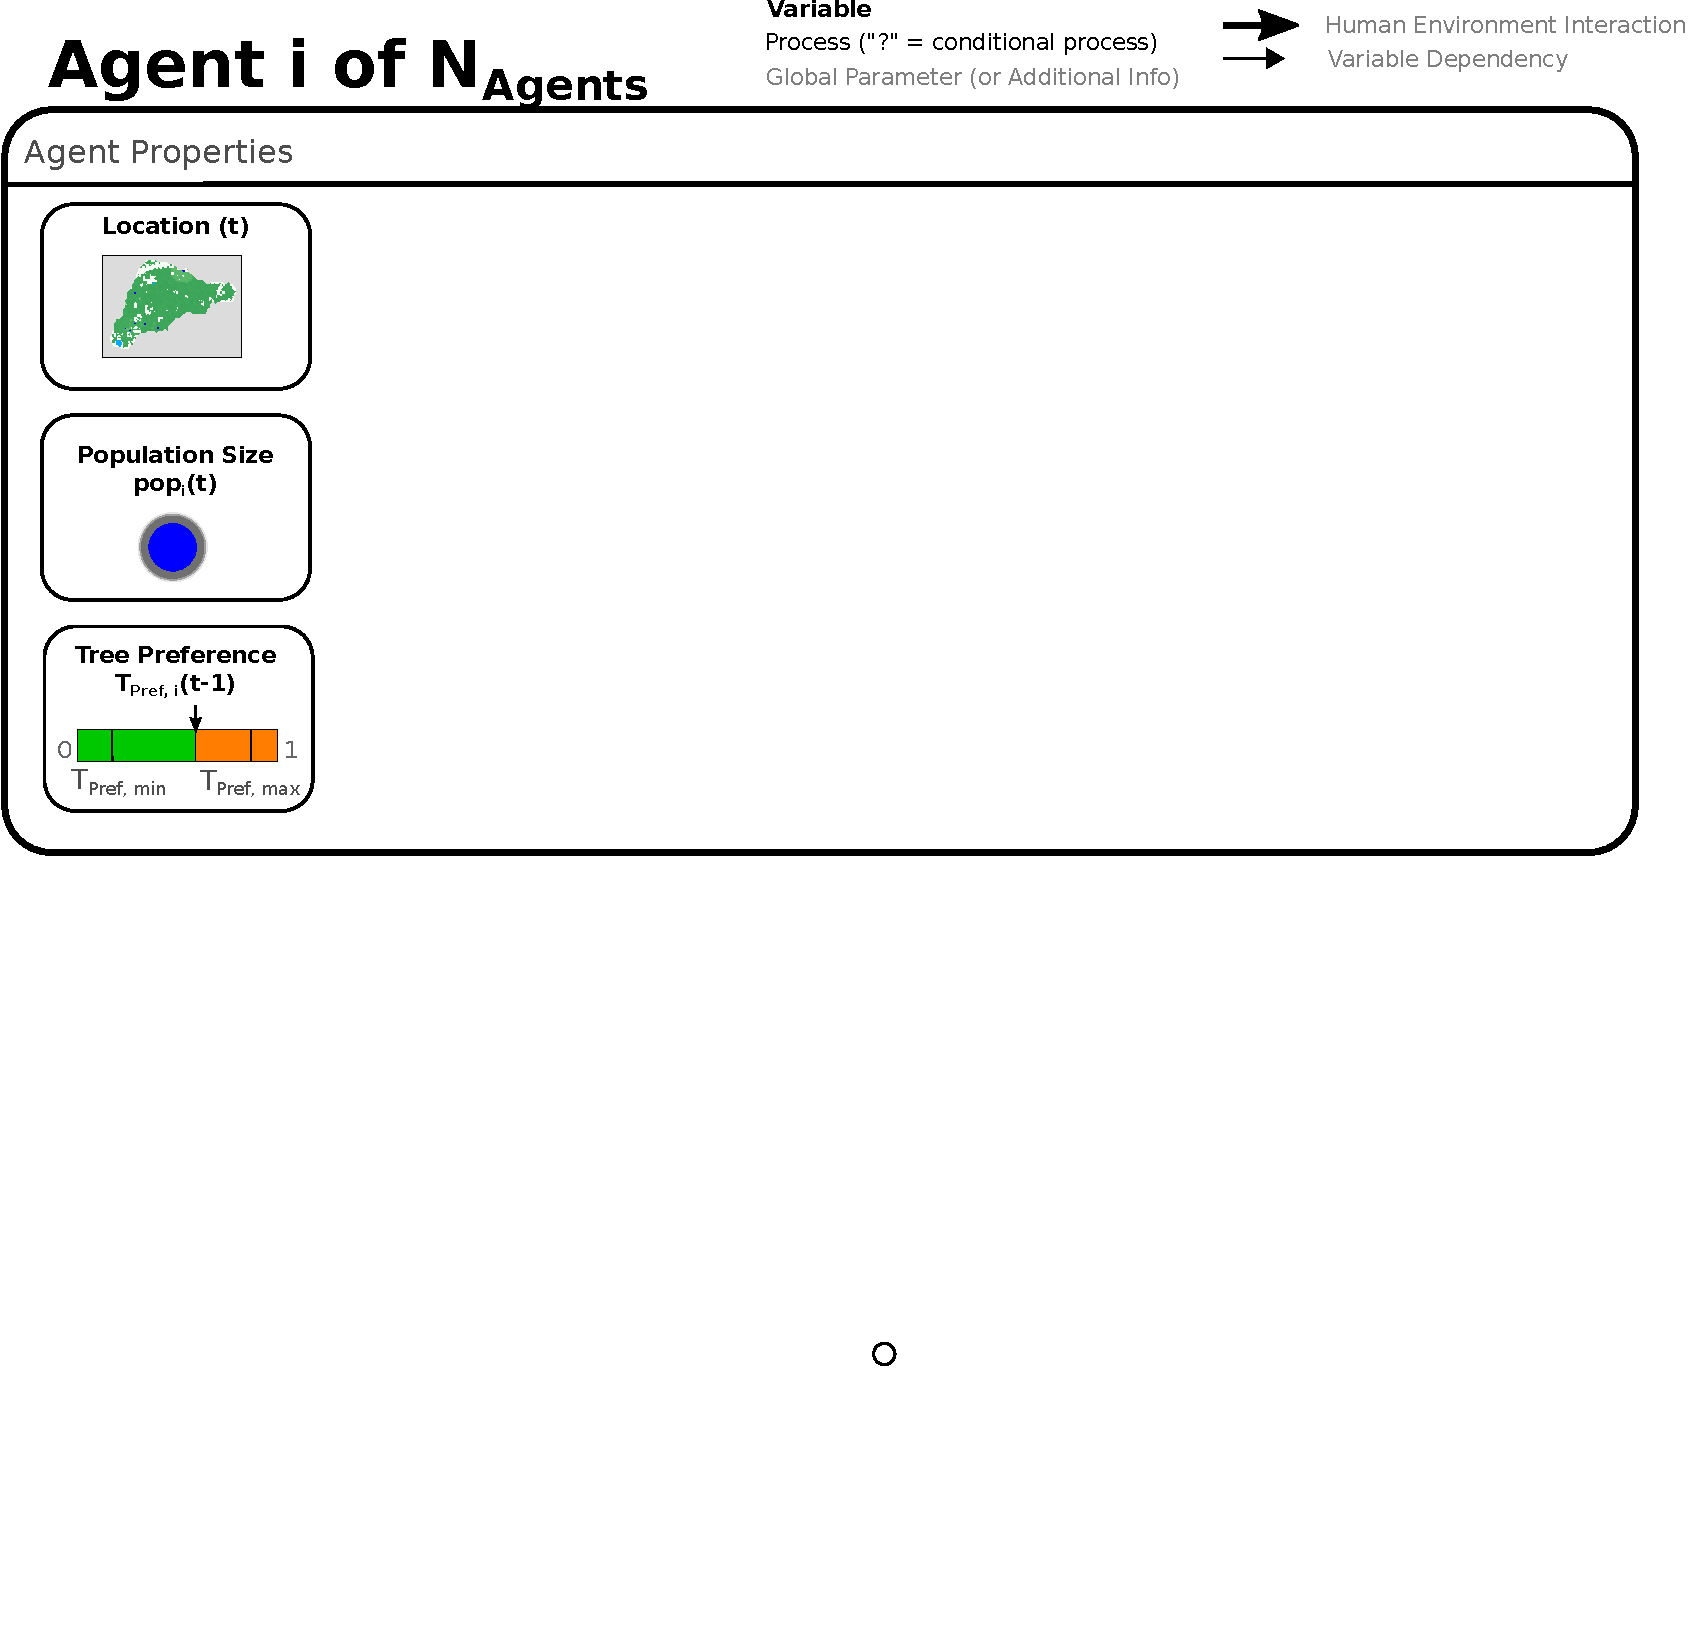
\includegraphics[width=0.85\linewidth]{SketchABM2/Agent_Props}}
\only<3>{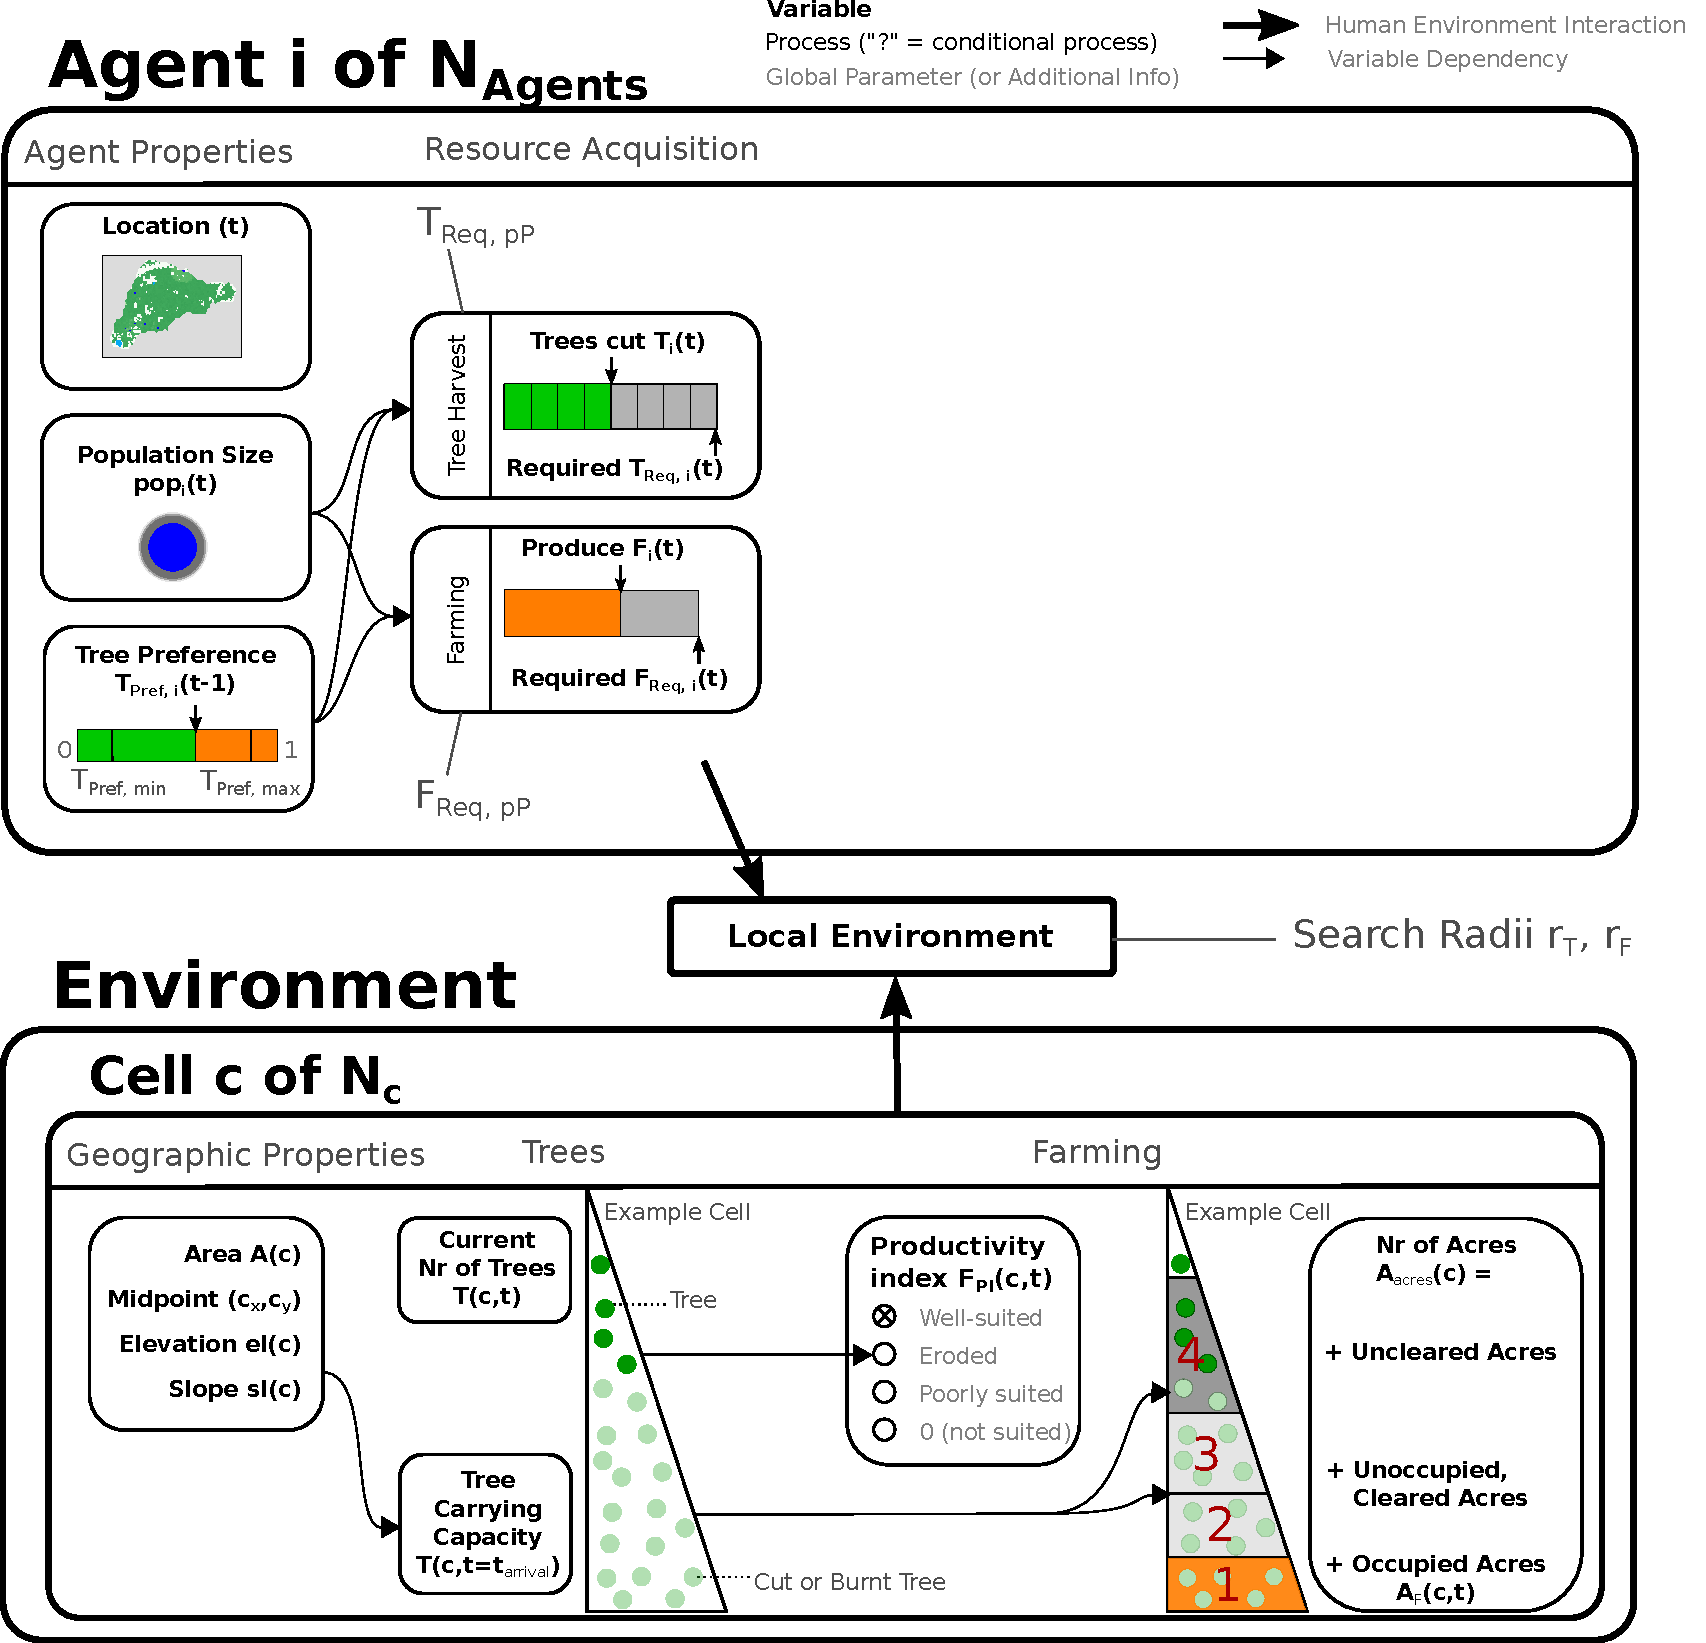
\includegraphics[width=0.85\linewidth]{SketchABM2/Agent_Harvest}}
\only<4>{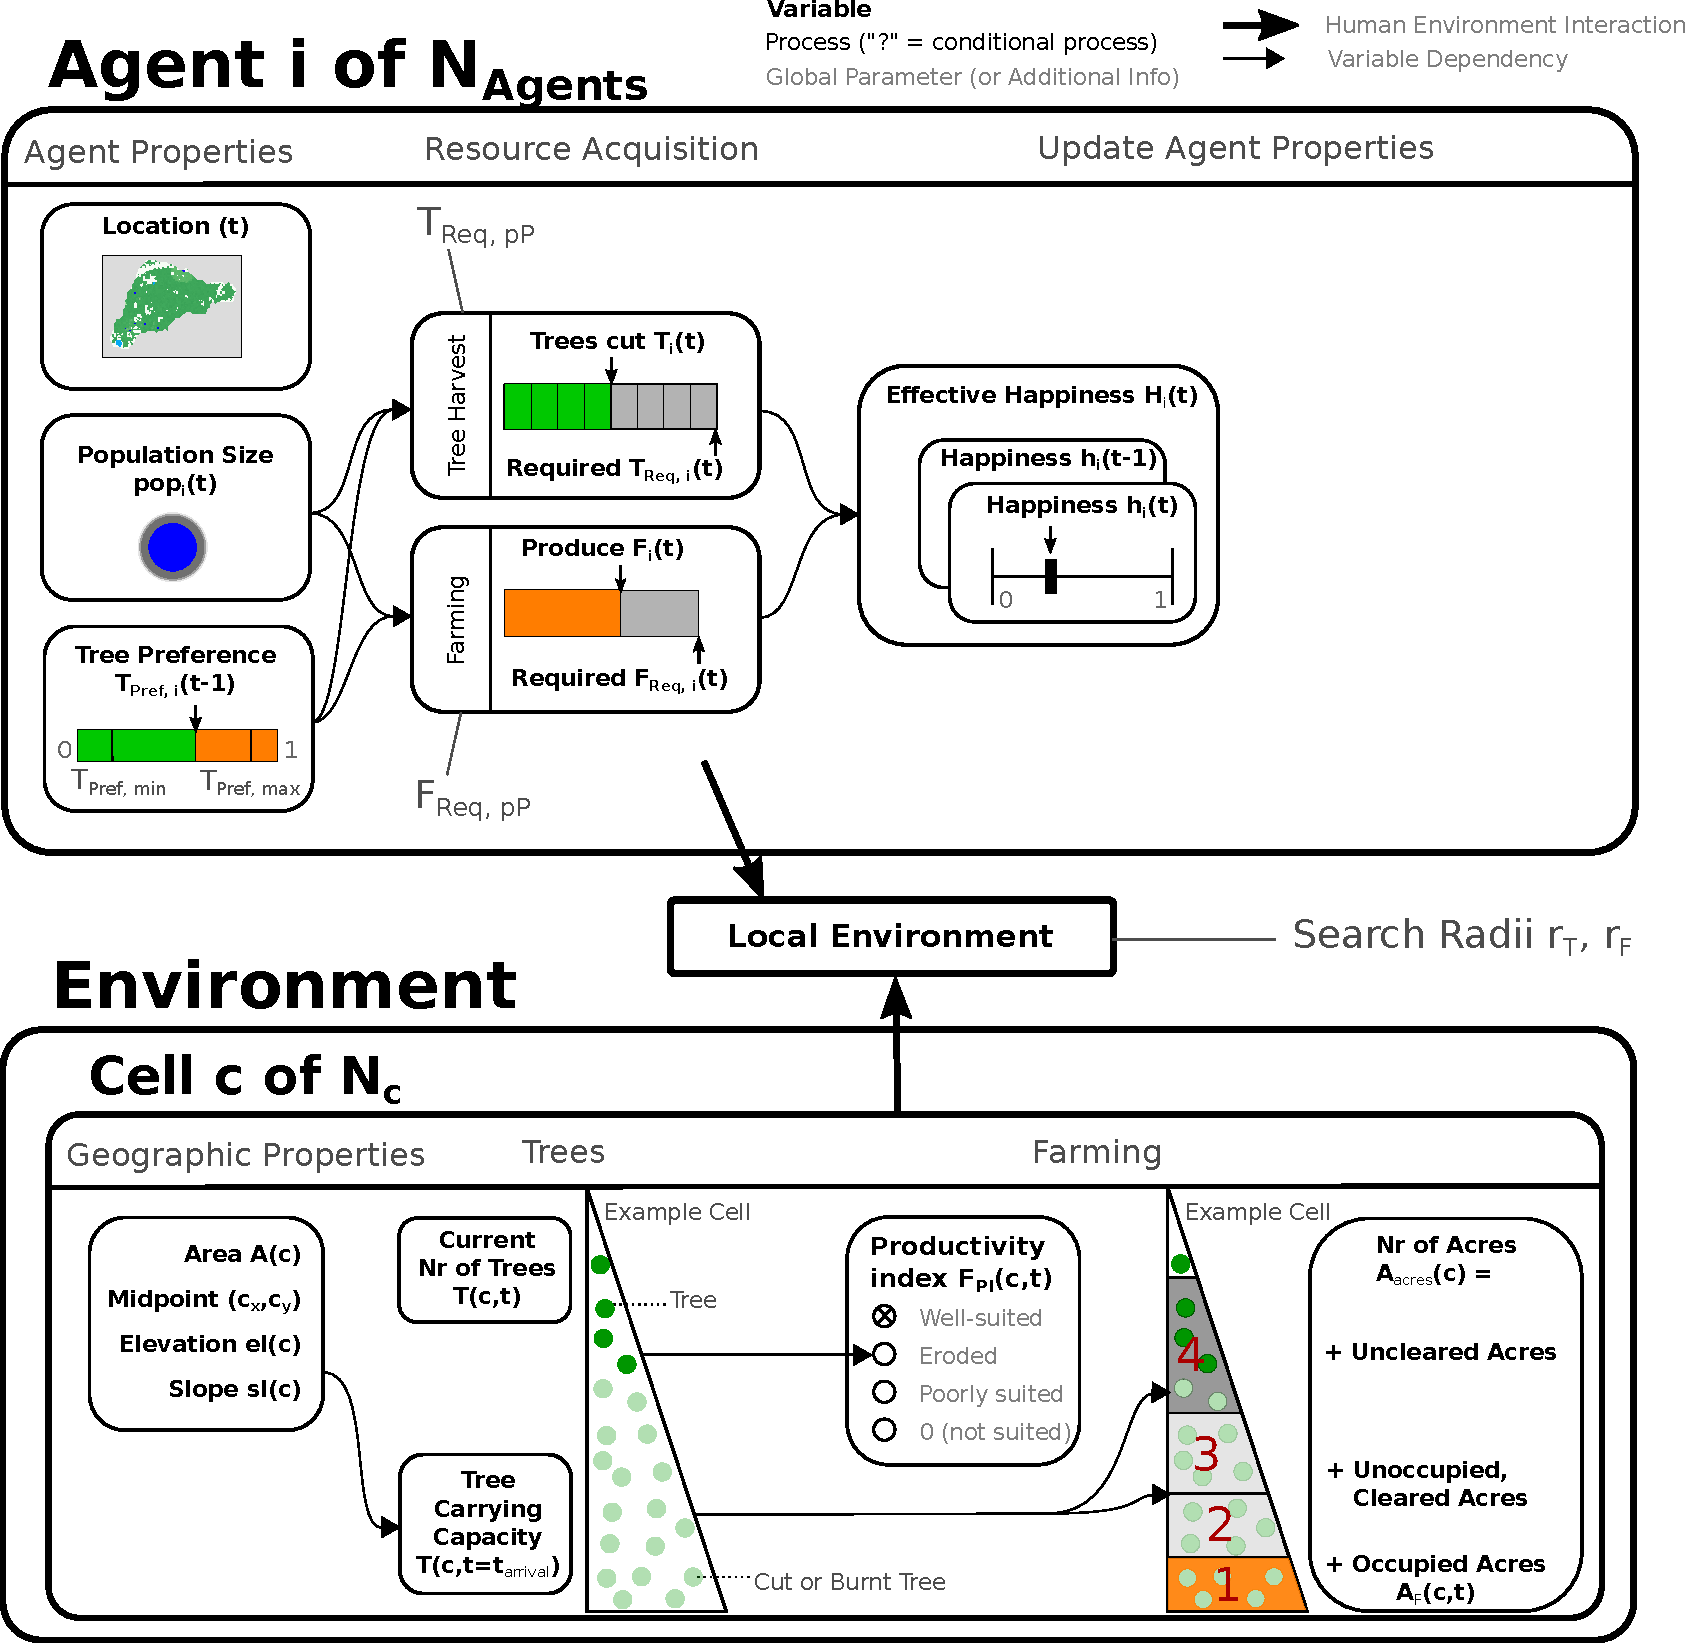
\includegraphics[width=0.85\linewidth]{SketchABM2/Agent_Update2}}
\only<5>{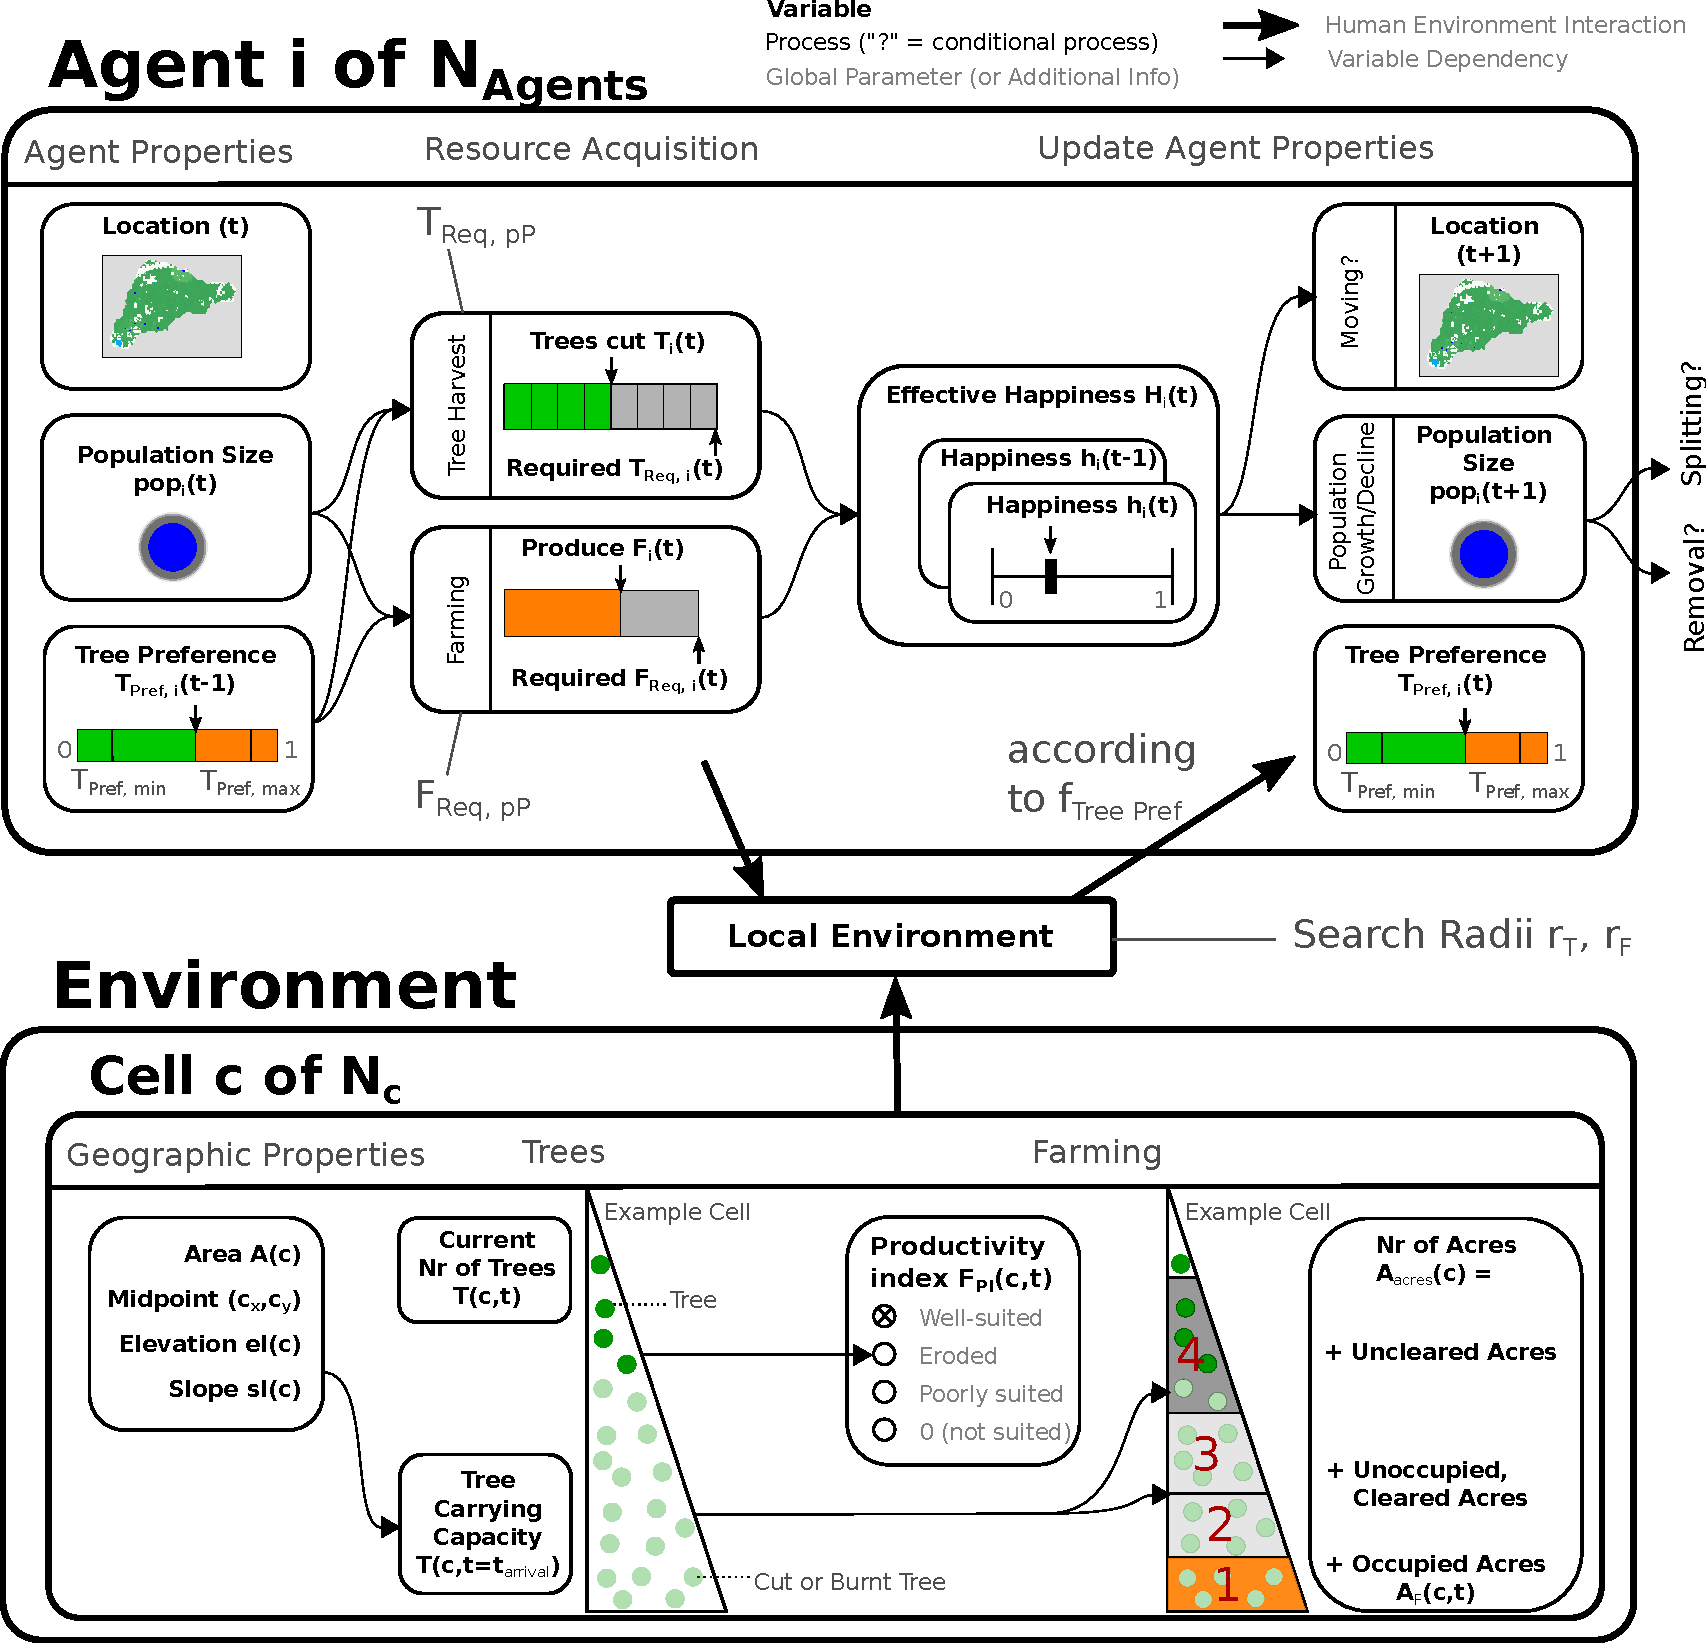
\includegraphics[width=0.85\linewidth]{SketchABM2/sketch_triangles}}
\end{frame}

%\begin{frame}
%Exceptions: Fishing.
%\end{frame}


\begin{frame}{Moving: Decision Making based on Penalties}

\begin{columns}
\begin{column}{0.2\textwidth}
	\centering
	\only<1>{
\includegraphics[height=2cm]{images/white}\captionof{figure}{\scriptsize \ \  }}
	\only<2->{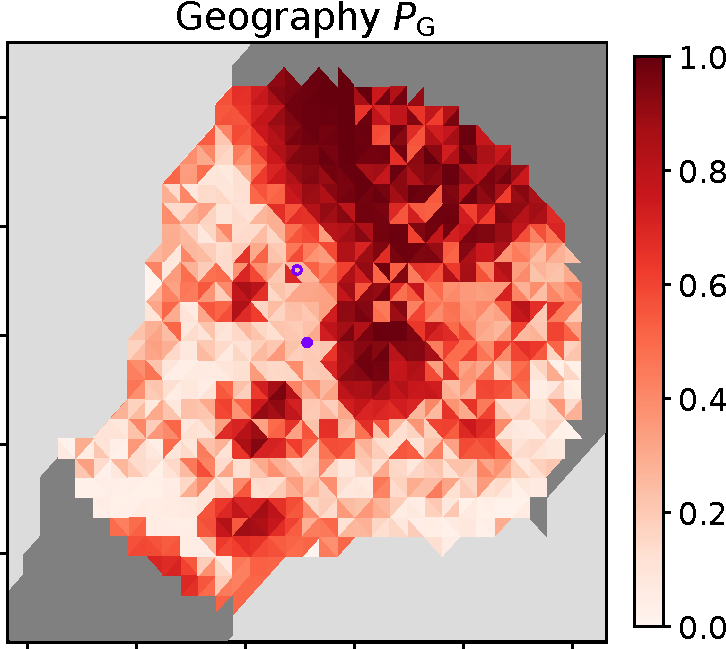
\includegraphics[height=2cm]{../../Thesis/images/Results/Standard/Penalties_AG500_t=1603_G}
	\captionof{figure}{\scriptsize Geography}}
\end{column}%\hfill
\begin{column}{0.2\textwidth}
	\centering
	\only<3->{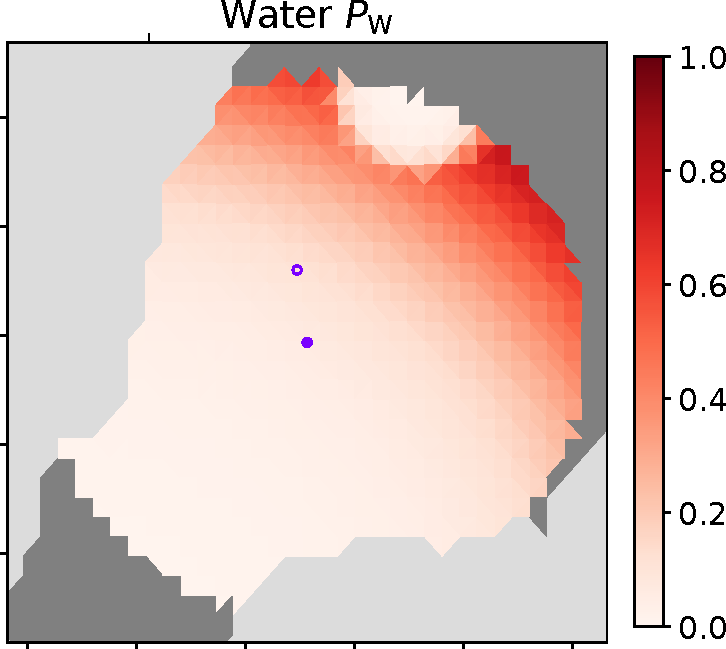
\includegraphics[height=2cm]{../../Thesis/images/Results/Standard/Penalties_AG500_t=1603_W}
	\captionof{figure}{\scriptsize Water}}
\end{column} 
\begin{column}{0.2\textwidth}
\centering
\only<4->{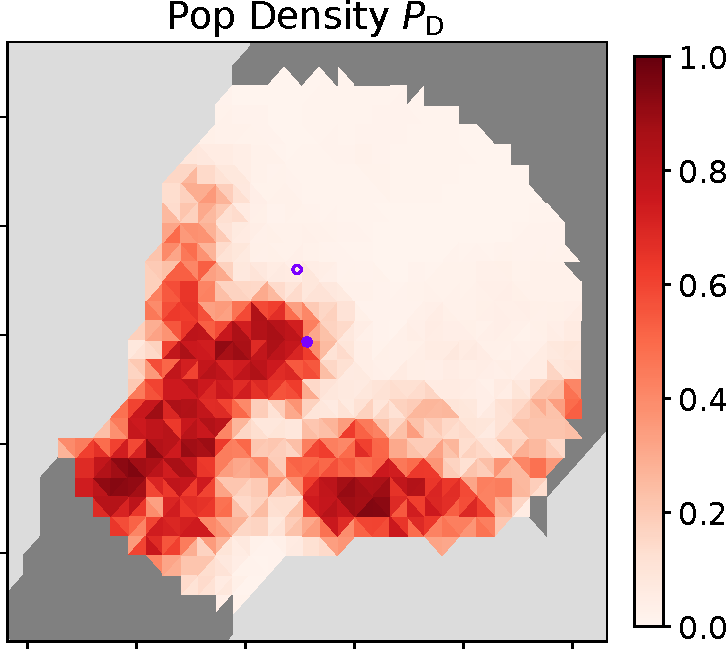
\includegraphics[height=2cm]{../../Thesis/images/Results/Standard/Penalties_AG500_t=1603_D}
	\captionof{figure}{\scriptsize Pop.\ Density}}
\end{column}
\begin{column}{0.2\textwidth}
\centering
\only<5->{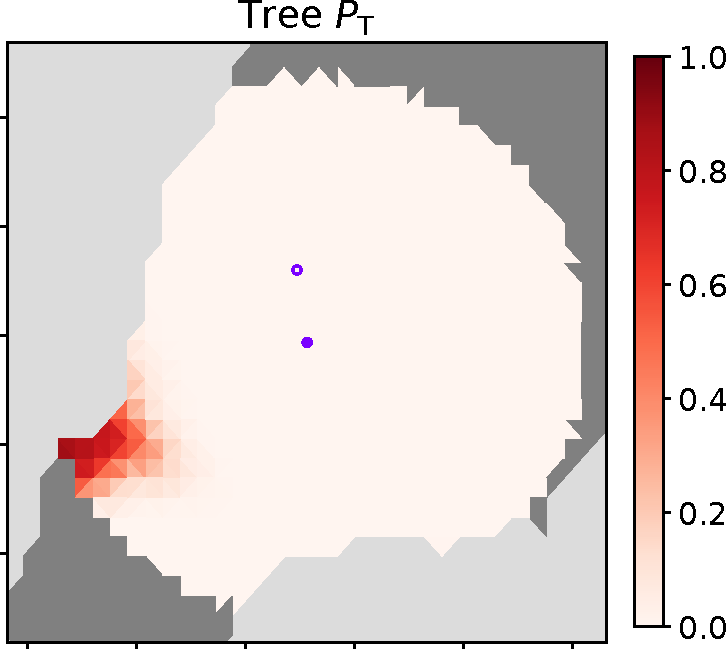
\includegraphics[height=2cm]{../../Thesis/images/Results/Standard/Penalties_AG500_t=1603_T}
	\captionof{figure}{\scriptsize Trees}}
\end{column}
\begin{column}{0.19\textwidth}
\centering
\only<6->{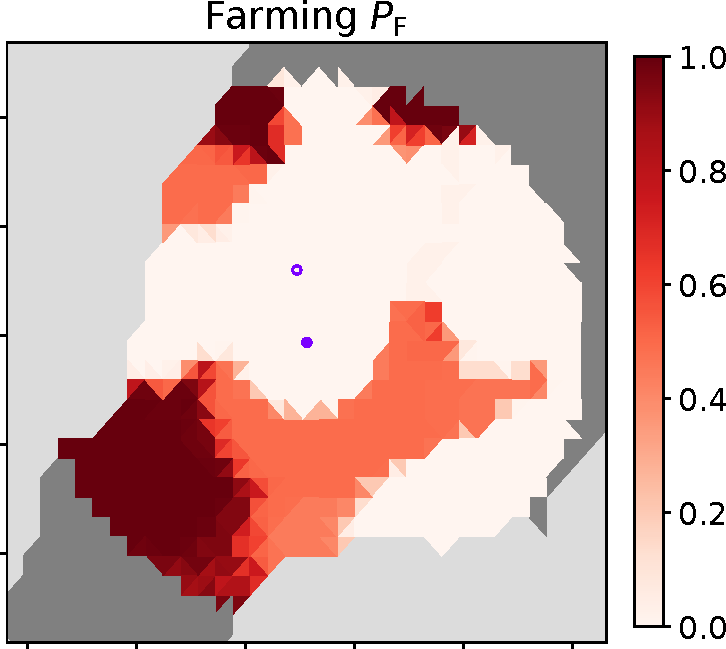
\includegraphics[height=2cm]{../../Thesis/images/Results/Standard/Penalties_AG500_t=1603_F}
	\captionof{figure}{\scriptsize Farming Sites}}
\end{column}
\end{columns}

\vfill
\centering
\begin{columns}
	\begin{column}{0.35\textwidth}
		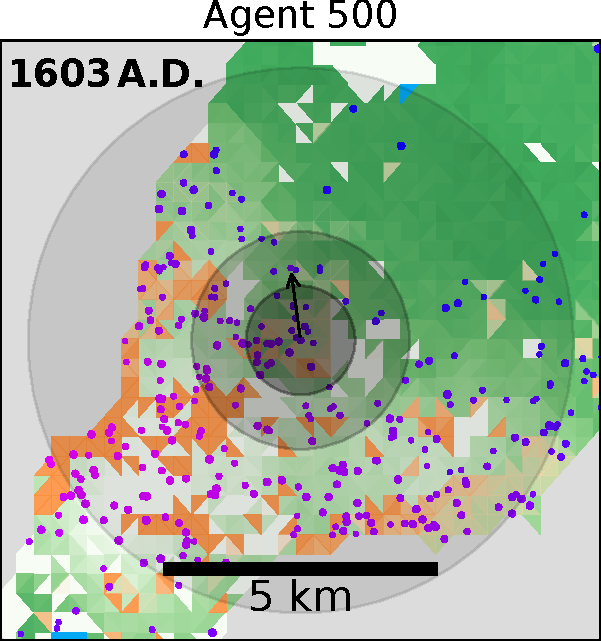
\includegraphics[height=4.5cm]{../../Thesis/images/Results/Standard/Penalties_AG500_t=1603_Situation}
	\end{column}
	\begin{column}[t]{0.25\textwidth}
	 	\only<2>{\textbf{Avoid cells...\\ ...
	  	with large elevation and large slope}}%
  		\only<3>{\textbf{Avoid cells...\\ ...
  				far from a (big) freshwater source   }}%
  		\only<4>{\textbf{Avoid cells...\\ ...
  				in regions with large population density}}%	
 			\only<5>{\textbf{Avoid cells...\\...
 					with few trees nearby  }}%
				\only<6>{\textbf{Avoid cells... \\ ...
						with few (well-suited) available farming sites nearby}}%
  		\only<7>{\textbf{\begin{center} {\Huge$\Downarrow$} \end{center} \ra \quad Total\quad \ra }}
  	
	\end{column}
	\begin{column}{0.35\textwidth}
		\only<2>{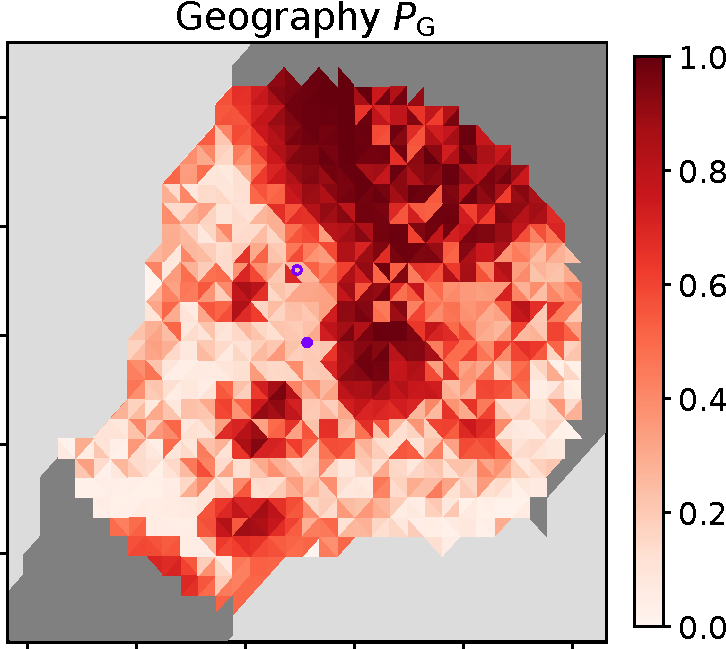
\includegraphics[height=4.5cm]{../../Thesis/images/Results/Standard/Penalties_AG500_t=1603_G}}%
		\only<3>{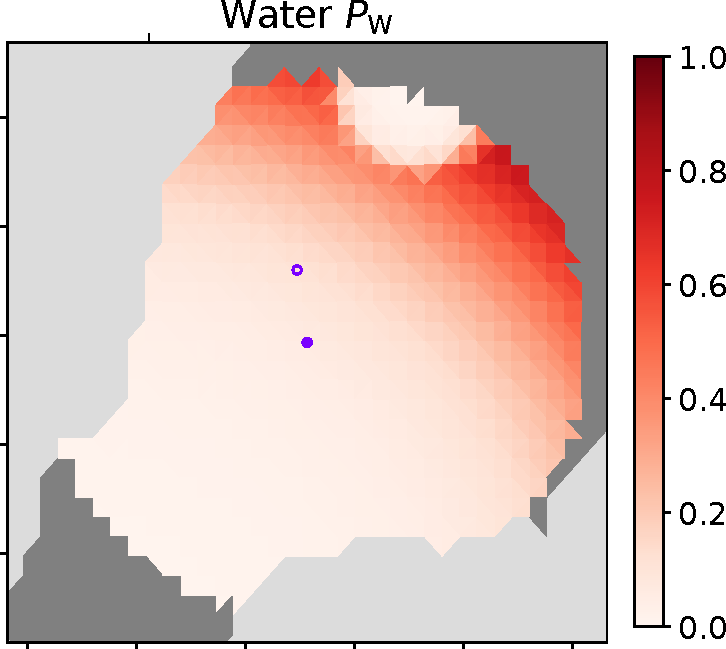
\includegraphics[height=4.5cm]{../../Thesis/images/Results/Standard/Penalties_AG500_t=1603_W}}%
		\only<4>{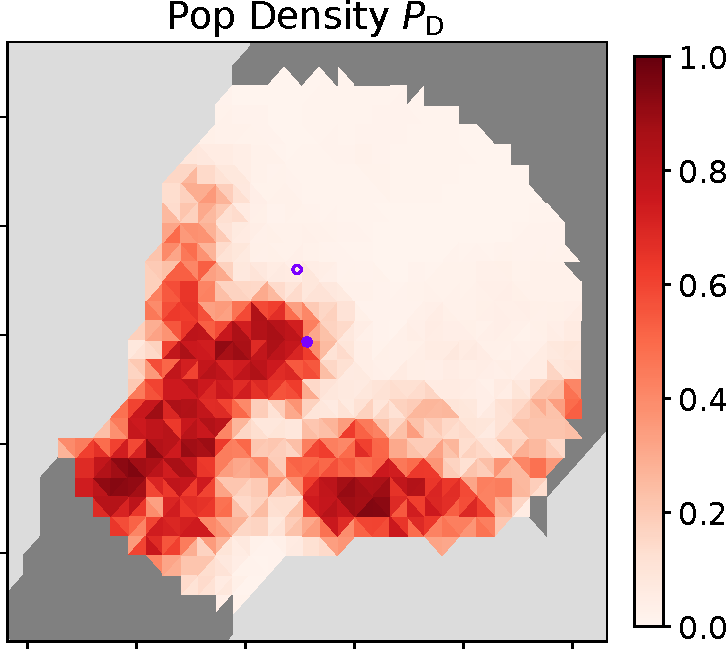
\includegraphics[height=4.5cm]{../../Thesis/images/Results/Standard/Penalties_AG500_t=1603_D}}%	
		\only<5>{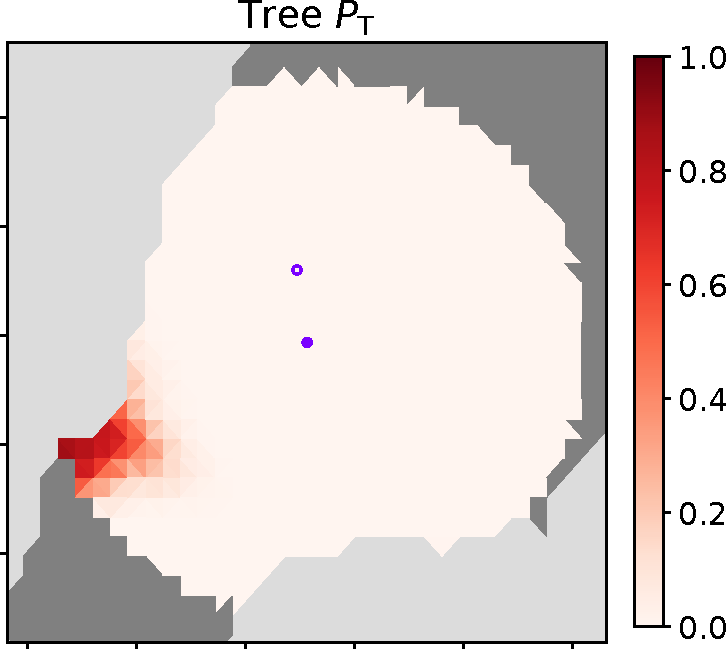
\includegraphics[height=4.5cm]{../../Thesis/images/Results/Standard/Penalties_AG500_t=1603_T}}%	
		\only<6>{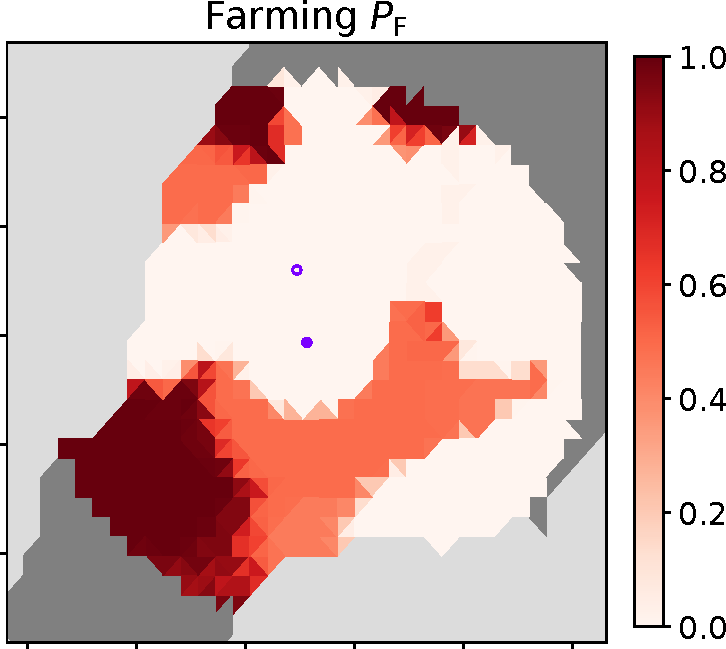
\includegraphics[height=4.5cm]{../../Thesis/images/Results/Standard/Penalties_AG500_t=1603_F}}%
		\only<7>{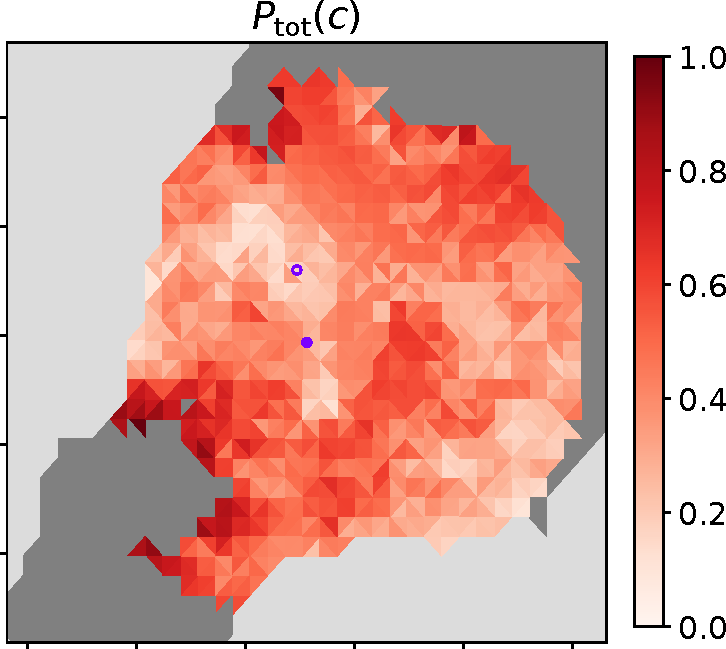
\includegraphics[height=4.5cm]{../../Thesis/images/Results/Standard/Penalties_AG500_t=1603_tot}}
	\end{column}
\end{columns}
%

\end{frame}


\begin{frame}{The Full Model}
\begin{columns}
	\column[T]{0.69\textwidth}
		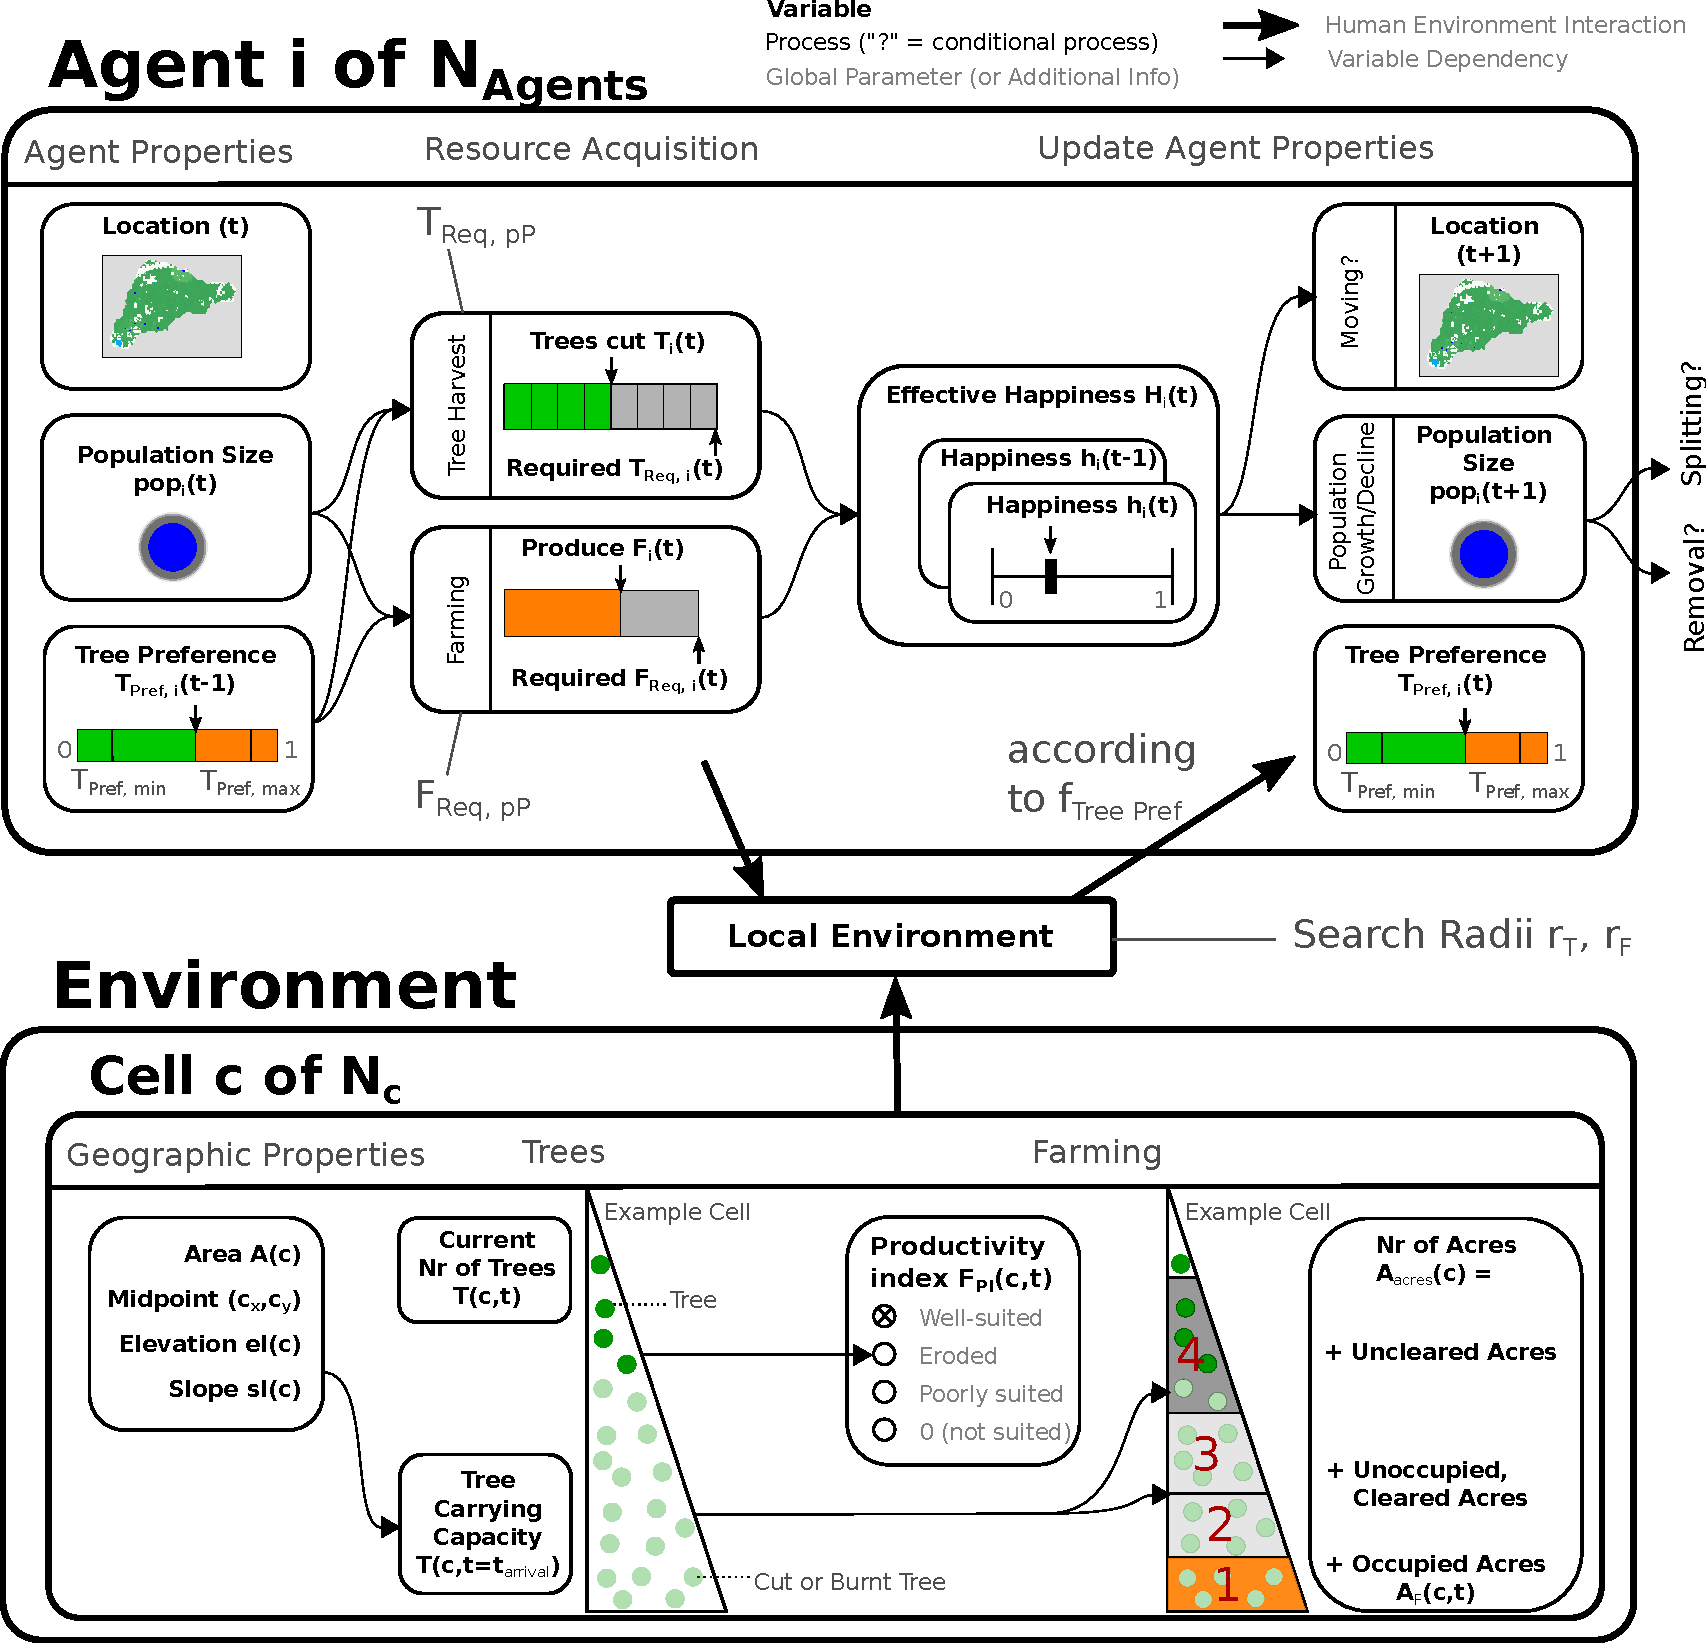
\includegraphics[height=0.85\textheight]{SketchABM2/sketch_triangles}
	\column[T]{0.29\textwidth}
		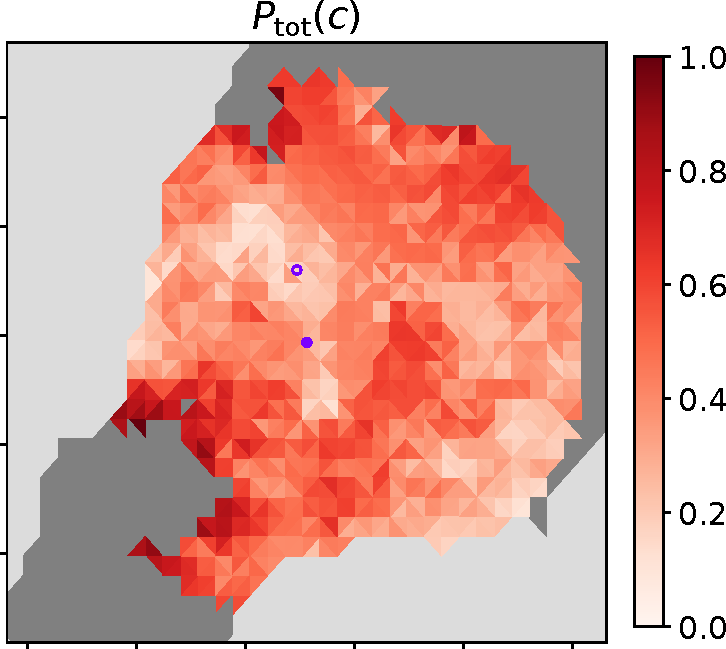
\includegraphics[height=3.5cm]{../../Thesis/images/Results/Standard/Penalties_AG500_t=1603_tot}
\end{columns}
\end{frame}
	




\section{Results and Discussion}
% !TEX root=frame_thesis.tex
\chapter{Results and Discussion}\label{chapter:Results}
\FloatBarrier
\section{A Standard Configuration Run}\label{sec:std} 
\paragraph{Overview of the Results.}
The standard configuration run results of the ABM presented in Section \ref{chapter:Methods} are produced with parameters presented in Table \ref{tab:sensitivity}.
Figure \ref{fig:STDrull} presents snapshots of a simulation showing the spatial pattern of trees, farmed sites, and agents (with their tree preferences) at different times.
In the supplementary material, I provide a link to an animated Figure showing the evolution of these spatial patterns over time.
Since multiple processes in the model are stochastic, each run with a specific seed is a unique realisation.
In order to obtain statistically valid aggregate results, I use an ensemble of $15$ runs for all experiments.
Adding more runs (e.g.\ 20 or 25) does not significantly change the coefficient of variation for the ensemble over time (see Figure \ref{fig:coeffofvariation}).
The mean and standard deviation of the aggregated variables of this ensemble and their change over time is shown in Figure \ref{fig:STDstats}.
The uncertainty in the ensemble runs results from slight differences in the timing of the dynamics due to different realisations of the discrete, stochastic population growth process (see also Figure \ref{fig:realisationsofpopgrowth}). 
Hence, the peaks of the population sizes of single runs are at a similar level but slightly shifted in time. 
However, due to this shift the resulting ensemble mean (thick line in Figure \ref{fig:STDstats}) slightly underestimates the peak population size.

\begin{figure}
	\centering
	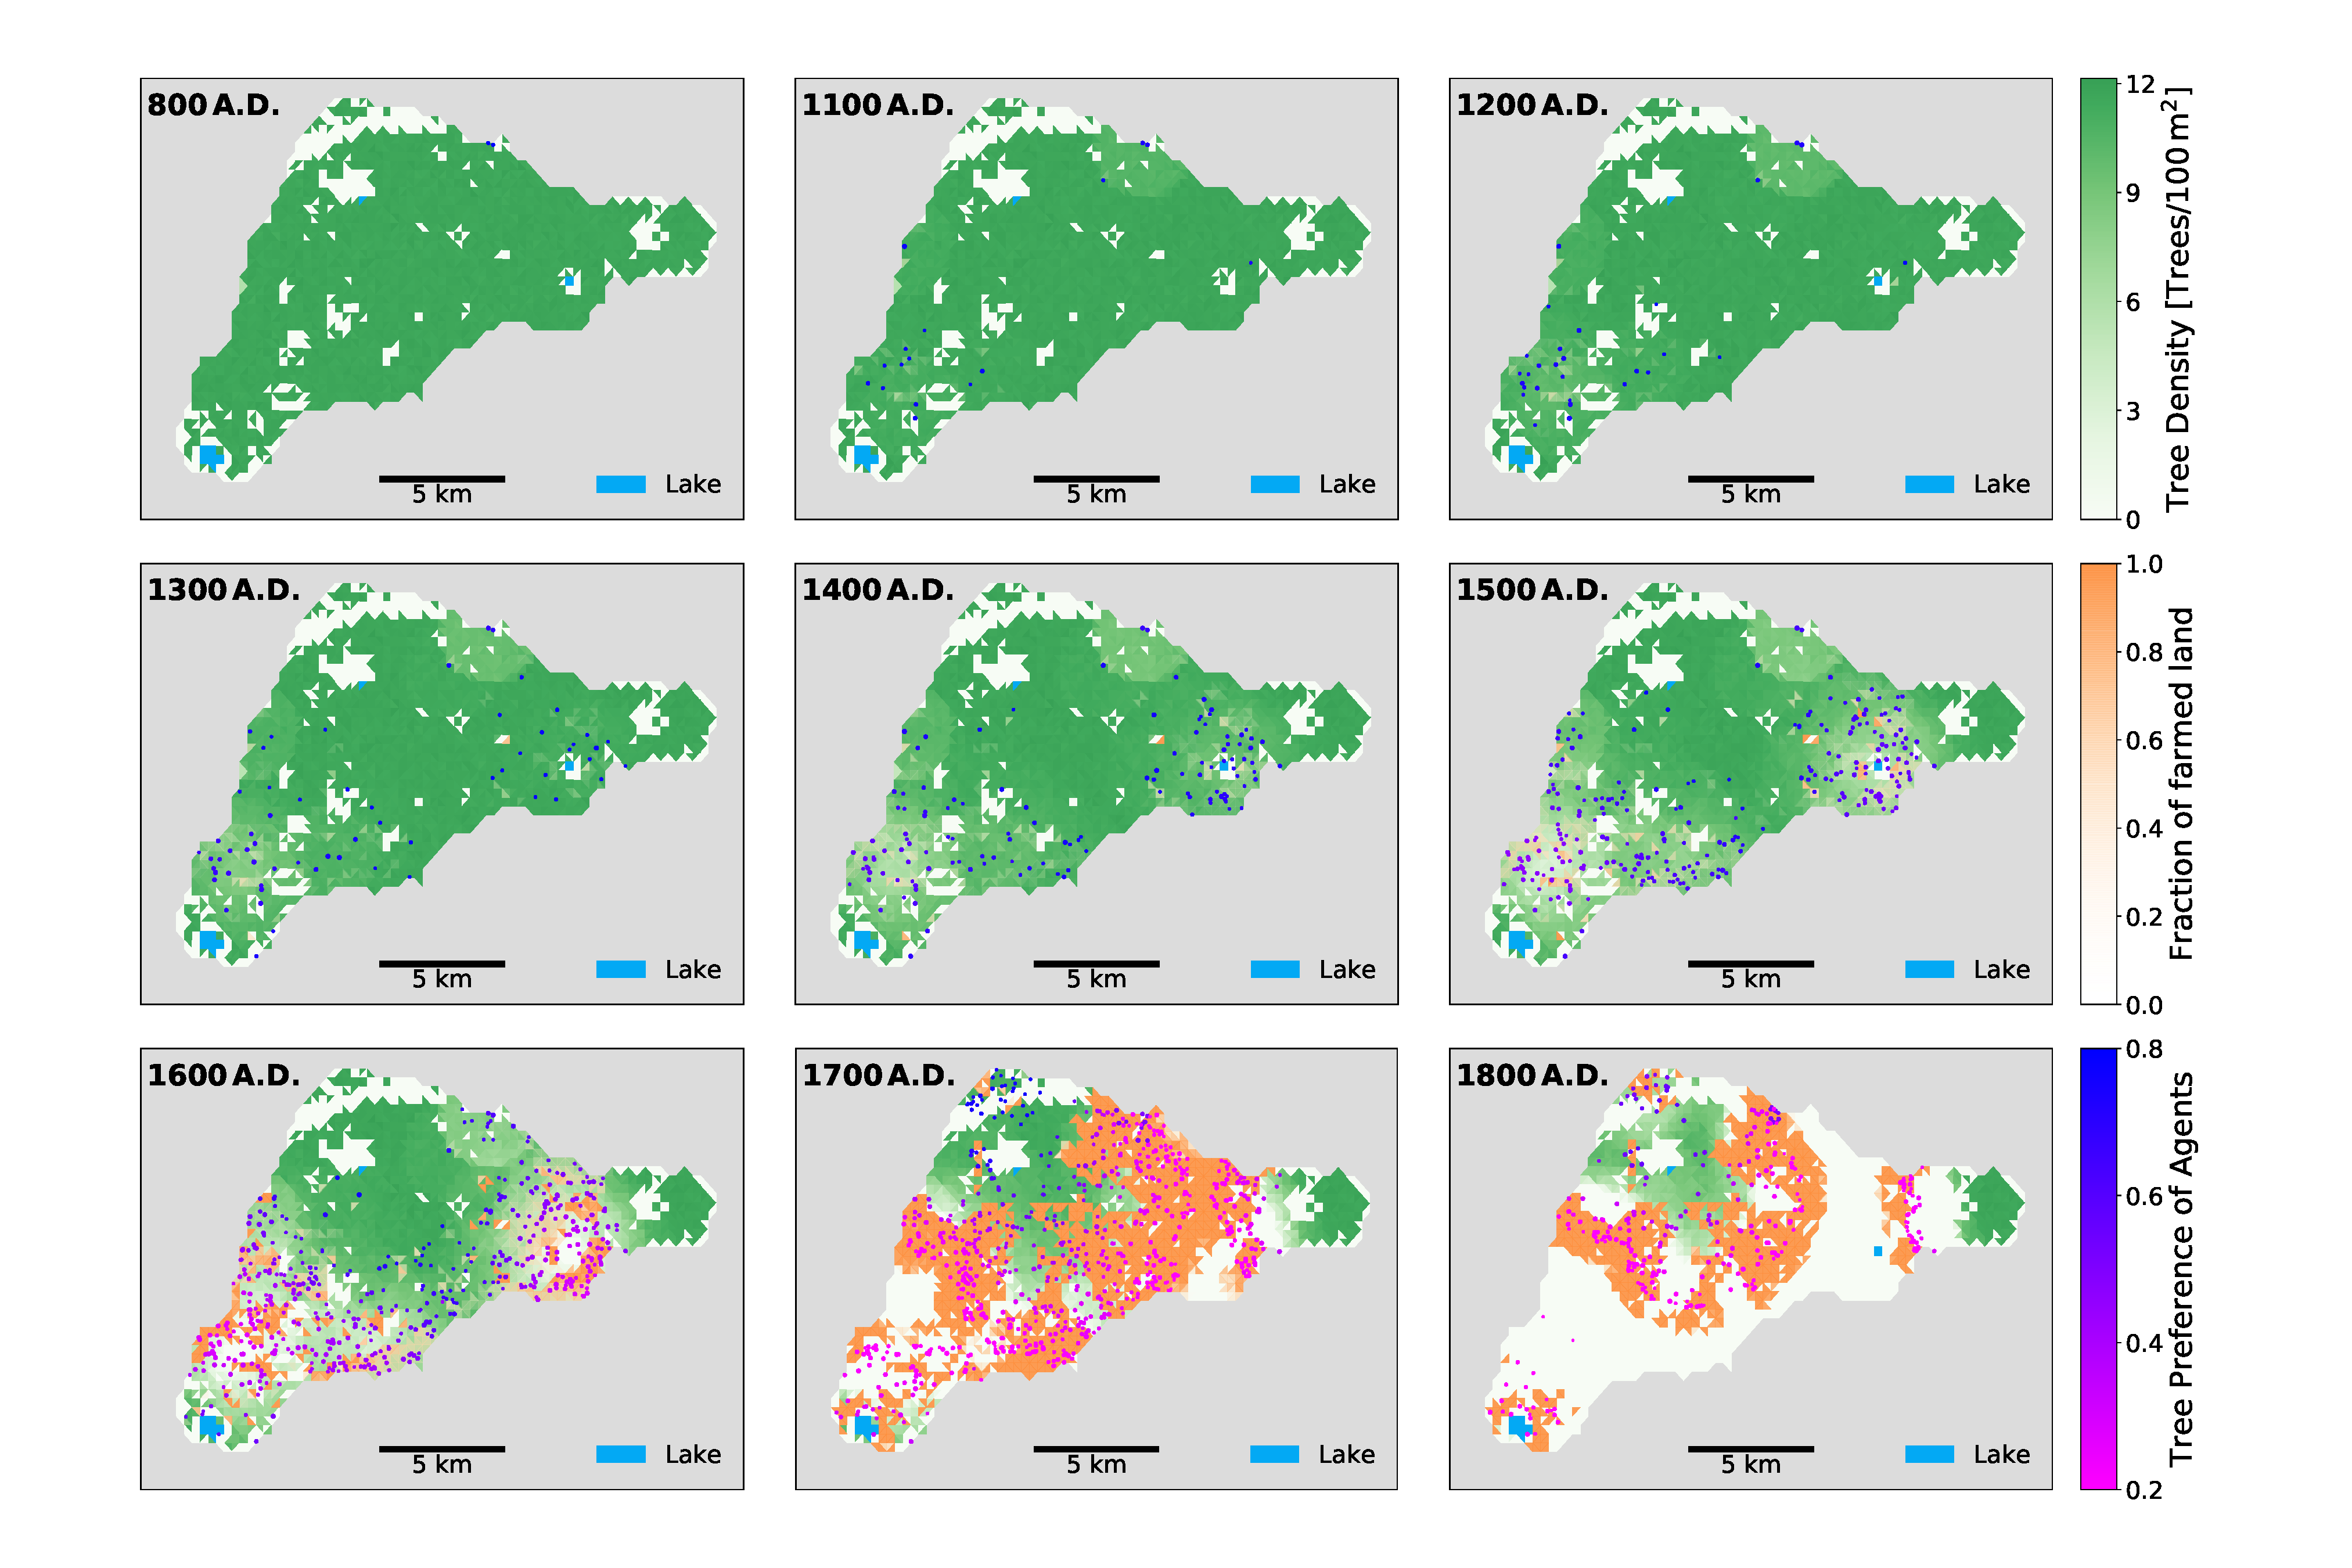
\includegraphics[width=1.3\textwidth, center]{images/Results/Standard/Rull2020_Comparison_seed3}
	\caption{Spatial patterns produced by the ABM in the standard run configuration at nine different times (comparable to Figure 9 in \citen{Rull2020}). The map shows the tree density in green and the fraction of farmed land in orange. Agents are represented by dots with a colour corresponding to their tree preference and size corresponding to their population size. They settle on the island and interact with the environment by cutting trees and turning arable land into farmed sites.}
	\label{fig:STDrull}
\end{figure}


\begin{figure}
	\centering
	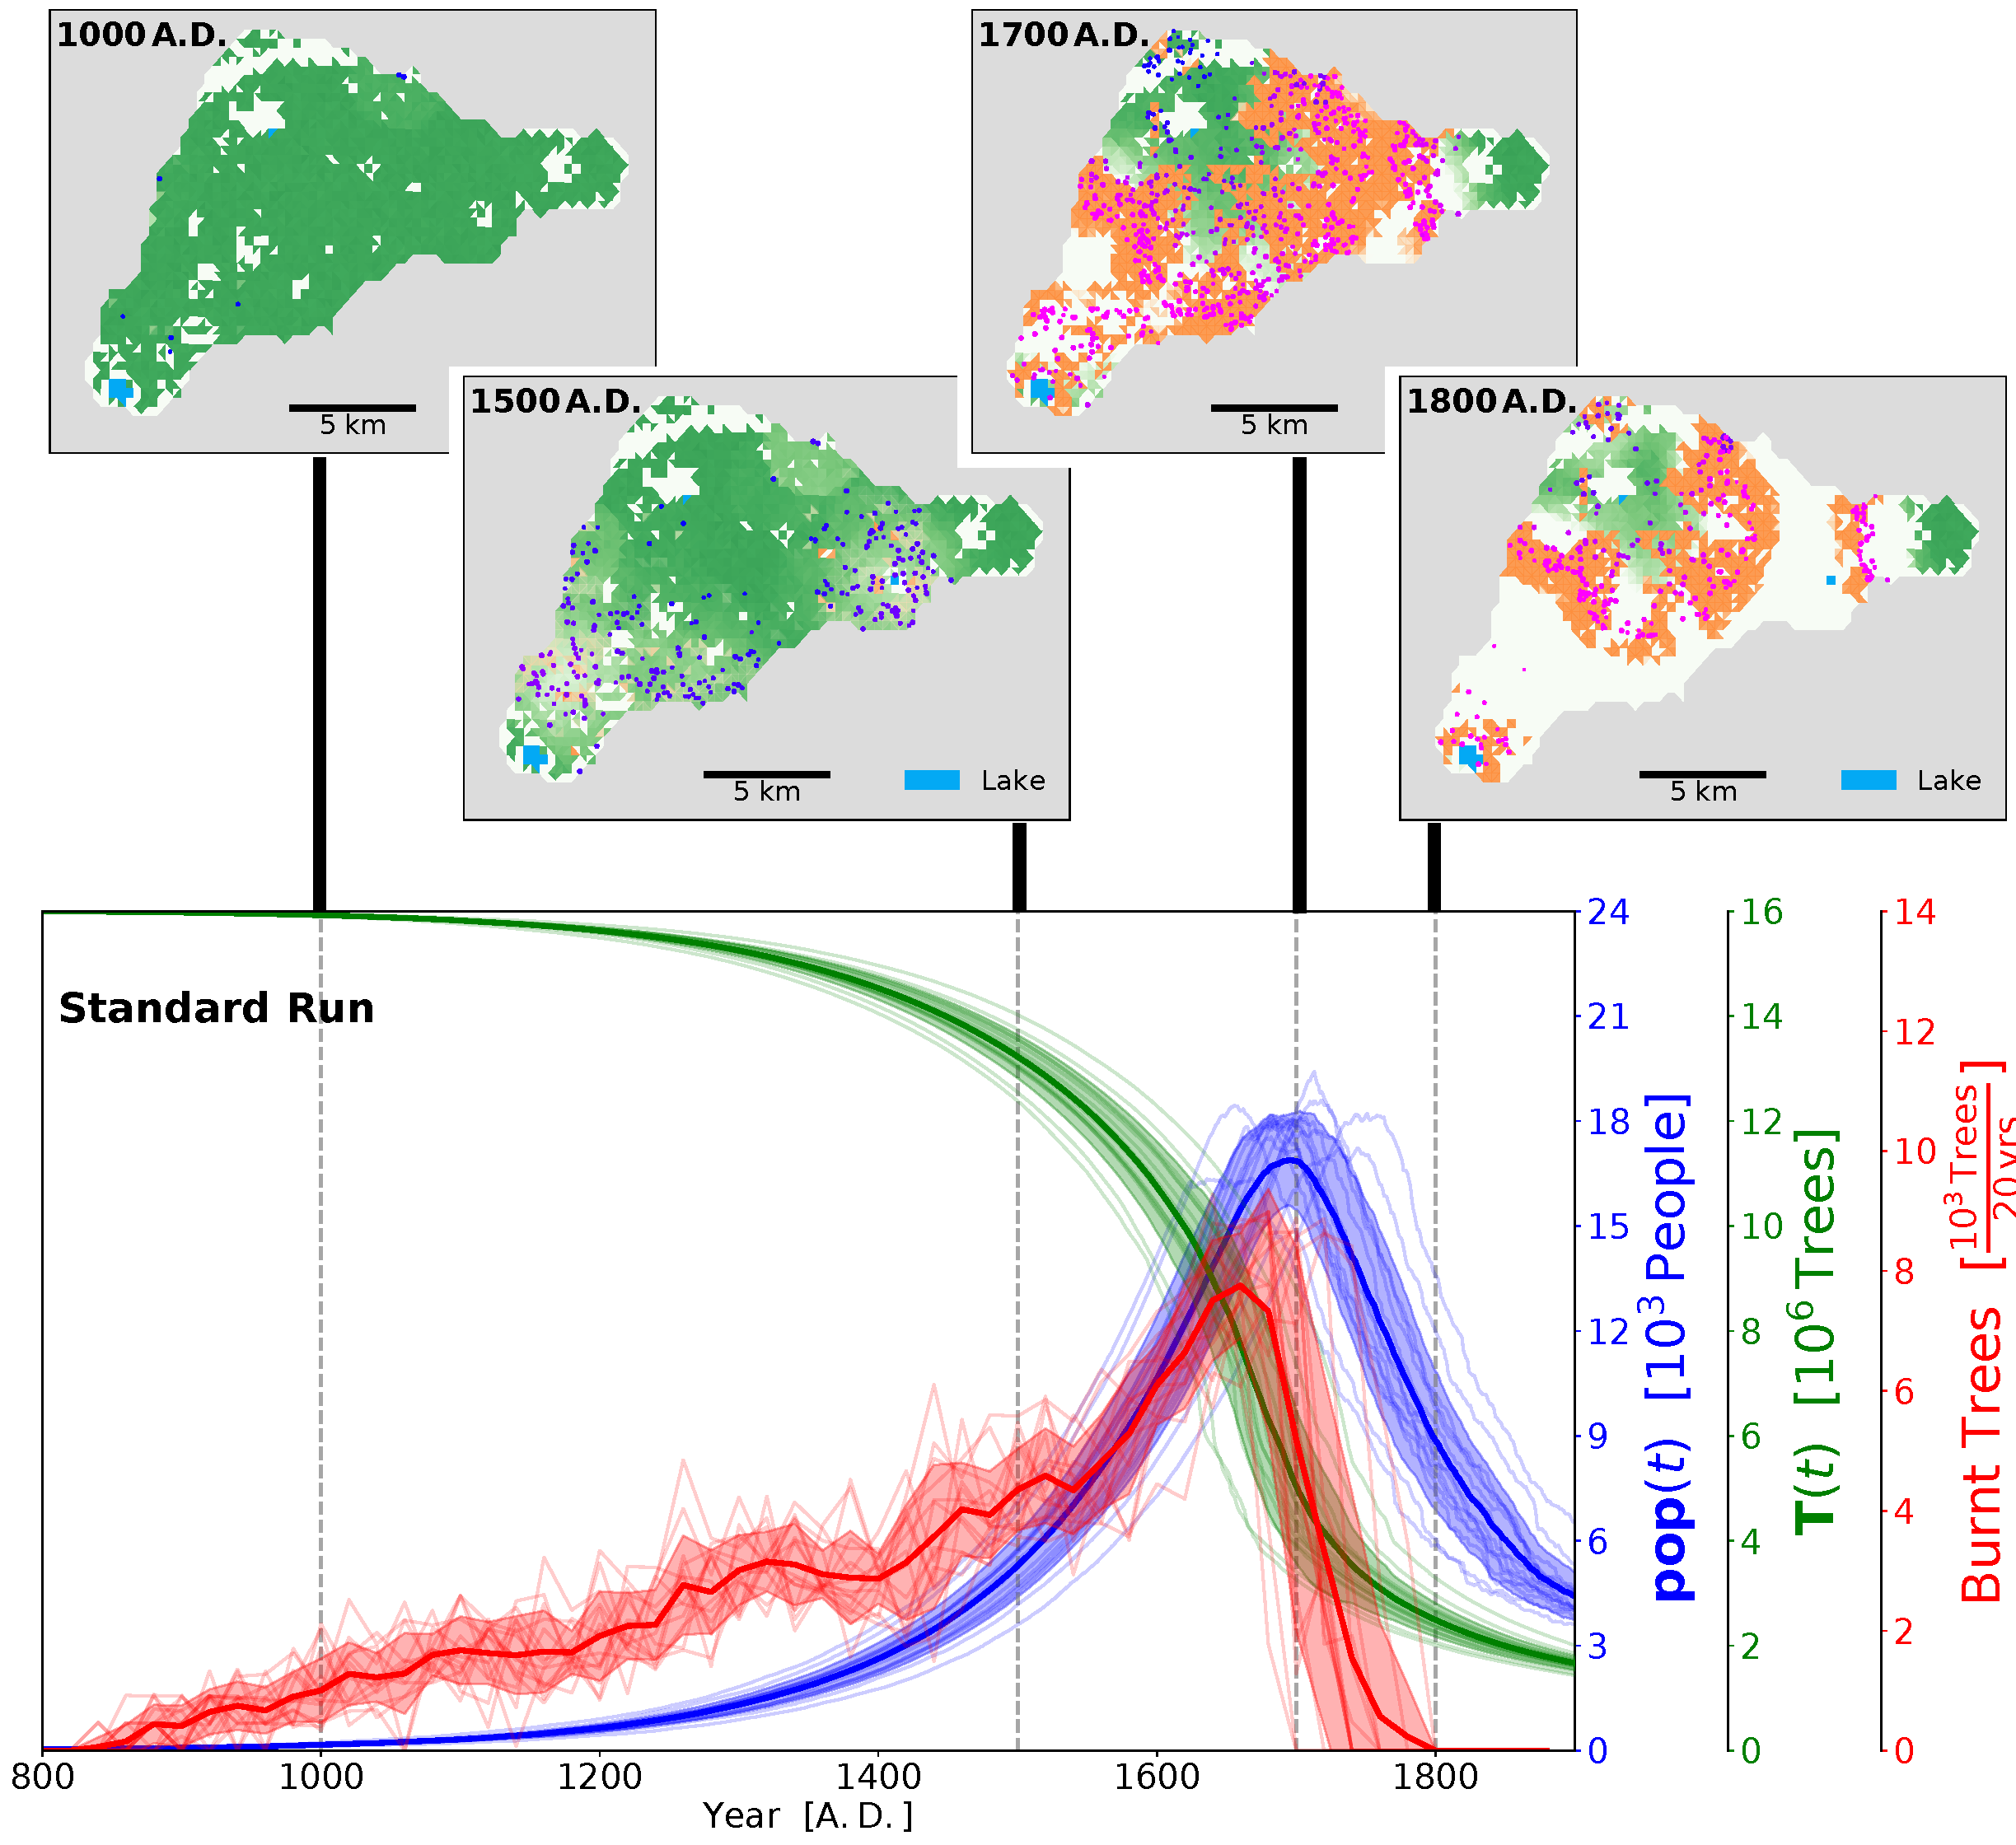
\includegraphics[width=1.\linewidth, center]{images/Results/Standard/EnsembleStatistics+Panels}
	\caption{
		Dynamics of aggregate population size, trees, and burnt trees in the standard run configuration. 15 different realisations (thin lines) are used to obtain the ensemble means (thick lines) and standard deviations (shaded areas). 
		The number of burnt trees is presented in bins of 20 years, as its variation is strong.
		The maps above show the spatial distribution of trees, farming and agent settlements with their tree preferences for one of these realisations (with the same colour coding as in Figure \ref{fig:STDrull}).}
	\label{fig:STDstats}
\end{figure}


\paragraph{The first phase: Initial Growth.}
In the beginning of the simulation, two agents with 20 individuals each settle at Anakena Beach (in the North in Figure \ref{fig:Karte}). 
The local tree density is at the carrying capacity (in total $16\cdot 10^6$ trees) and, thus, the agents' tree preference is high (blue colour in Figure \ref{fig:STDrull}).
In the first phase of the simulated time period, the agents' population size grows at a constant maximum growth rate, because trees and arable land are both abundant. 
Consequently, the number of agents increases and new agents start to colonise the rest of the island. 
Until the end of the first drought period in $1200\, {\rm A.D.}$, new agents tend to settle in the arable, coastal region South/South East of the island close to the major freshwater source Rano Kau. 
After $1200\, {\rm A.D.}$, also the region around Rano Raraku (in the West), now providing an alternative, low elevation freshwater source, is settled at rapid pace.
Agents linearly adapt their tree preference to the slow environmental change and, thus, intensify farming activity.
As Figure \ref{fig:STDstats} shows, the amount of burnt trees to clear land for agriculture also increases linearly in this phase.

\begin{figure}
	\centering
	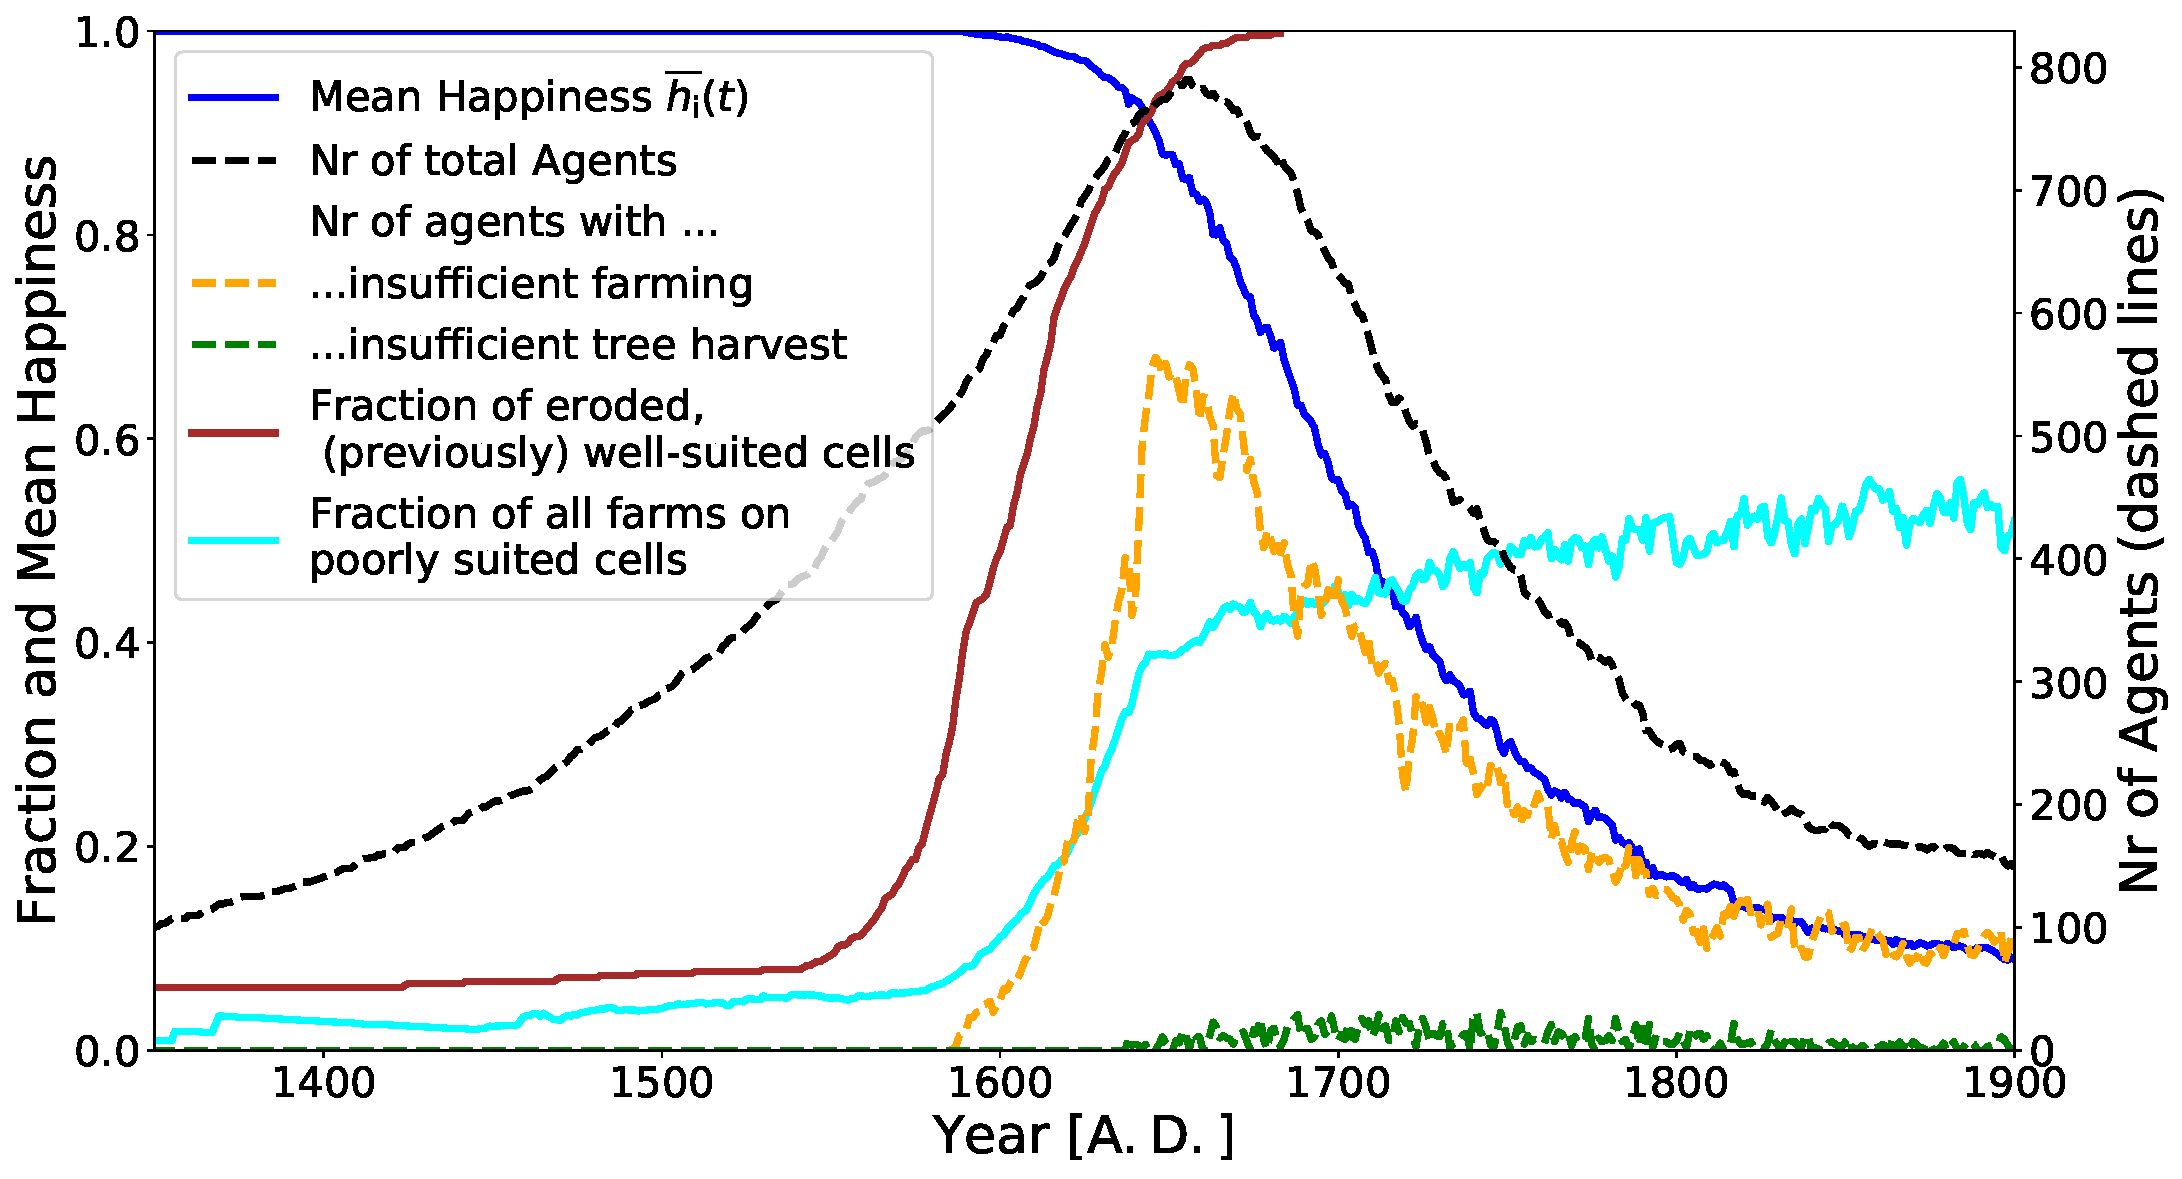
\includegraphics[width=\textwidth]{images/Results/Standard/StandardsecondaryStats}
	\caption{
		Indicators of the change from net growth to net decline in population dynamics for one single realisation in the standard run configuration.
	Dashed lines correspond to the y-axis on the right representing absolute number of agents.
	The blue line shows the mean happiness index of all agents. The black, dashed line shows the total number of agents. The number of agents that lack either sufficient land for farming or trees are shown in yellow and green, respectively. The brown line shows the fraction of cells (previously classified as well-suited for farming) with erosion due to complete deforestation. The cyan line shows the fraction of farming sites on poorly suited sites.}
	\label{fig:STDsecondayrstats}
\end{figure}

%Thereby, agents accelerate the depletion of the non-renewable resource, trees and, thus, in a self-enhancing loop, acquire more farming land.

%Further, this large-scale deforestation leads to a sharp increase of erosion of well-suited sites around $1650\, {\rm A.D.}$ and, hence, agents can not fill their farming requirements.

% with the first agents not meeting their resource requirements.
%However, since both neither further arable sites are available in the densely populated coastal regions and trees are deforested entirely by the remaining agents, these previously well-suited settlement locations are abandoned and the agents turn to the mostly poorly suited upland areas causing a shift towards the interior of the island.
%With the first agents not meeting their farming requirements around 1650, occupation of upland poorly suited farming sites jumps from a negligible fraction in $1650$ to $40-59\%$ in 1700.
%Consequently, the amount of burned trees rises quickly and comes to a abrupt halt between 1700 and 1800.
%Due to the low productivity indices of these sites, the use of burning trees to clear more space rises sharply in this period.

\paragraph{The second phase: Acceleration.}
The second phase of the dynamics is characterised by accelerating, non-linear feedbacks as shown by several indicators (Figure \ref{fig:STDsecondayrstats}).
In a self-enhancing loop, population growth in the settlement centres leads to an intensification of deforestation, a consequent decrease of the agents' tree preferences, increase of farming requirements, more acquisition of farming sites (therefore, more burnt trees) and, thus, more intense deforestation.
Simultaneously, erosion accelerates the deforestation as the farming productivity of occupied land decreases and  more land needs to be acquired.
%of arable farming land increases, leading to declined farming efficiency and, thus, more farming sites required per agent.
The portion of eroded, previously well-suited cells jumps from less than $10\%$ of all well-suited sites in $1600\,{\rm A.D.}$ to $100\%$ by $1700\, {\rm A.D.}$ (brown curve in Figure \ref{fig:STDsecondayrstats}).
Consequently, the amount of trees burnt for clearing land rises sharply. %to roughly $8\cdot 10^3$ trees per $20 \, {\rm yrs}$.
In total, this acceleration of local resource use, leads to an abandonment of the previously used well-suited locations (constituting nearly $100\%$ of all farming activity in $1650\,{\rm A.D.}$) and to the colonisation of mostly poorly suited, interior, upland areas (accounting for $40\%$ in $1700\,{\rm A.D.}$, cyan line in Figure \ref{fig:STDsecondayrstats}).
%The share of farming activity on those poorly suited cells rises from a negligible fraction in $1650\, {\rm A.D.}$ to $40\%$ of all farming activity in $1700\,{\rm A.D.}$ (cyan line in Figure \ref{fig:STDsecondayrstats}).
%However, there is no year in which all available farming sites are occupied simultaneously.
%However, the lower productivity indices in the poorly suited sites, leads to a further increase in land acquisition and, thus, deforestation. 

\paragraph{The third phase: Population Decrease.}
The third phase is characterised by a population decline and a substantial shift in the settlement patterns.
While in $1700\,{\rm A.D.}$ more than half of the agents experience some minor shortage in farming products (yellow curve in Figure \ref{fig:STDsecondayrstats}), 
%there is no time when all arable spaces are farmed simultaneously.
the loss of the trees, experienced by a few agents each year (green line in Figure \ref{fig:STDsecondayrstats}) triggers an exponential decline in averaged happiness, $\overline{h_{\rm i}(t)}$, just after $1700\, {\rm A.D.}$ (blue line in Figure \ref{fig:STDsecondayrstats}).
This leads to a period of intense moving.
Figure \ref{fig:penaltiesag500t1603} shows examples of an agent's penalties while searching for a new settlement location.
\begin{figure}
	\centering
	\includegraphics[width=1.3\linewidth, center]{images/Results/Standard/Penalties_AG500_t=1603_rad}
	\caption{Decision making in the moving module of an agent at time $1603\, {\rm A.D.}$ in the South Eastern portion of the island. 
		Each panel shows the same region of interest with the location of the agent in the centre (filled dot) and the new location after the decision is made (unfilled dot).
		The upper left panel shows the agent in its current local environment, indicated by circles with the radii $r_{\rm F}$, $r_{\rm T}$, and $r_{\rm M}$ (after the moving restriction). The upper middle panel shows the total penalty ($\in [0,1]\cup \infty$), and upper right the corresponding probability for the agent to move to each allowed cell. The remaining panels show the penalties in all categories ranging from $0$ to $1$.
		The lower right panel also shows the cells that are excluded from the search because they do not fulfil the necessary condition for tree and farming availability (black cells inside the $r_{\rm M}$ circle).}
	\label{fig:penaltiesag500t1603}
\end{figure}
This phase marks the end of net exponential growth for the population, which peaks at around $18\cdot 10^3$ people around $1700\, {\rm A.D.}$.
Within a relative short time period of less than $50$ years, the population starts to decrease exponentially with a growth rate of $-0.5$ to $-1\%$ (see Figure \ref{fig:app:STDnetgrowthrate} in the Appendix).
The population decreases despite the fact that there are always both unoccupied farming sites and sufficient total number of trees on the island.
However, since the harvest is confined to the local surrounding of an agent in a specific location, it typically lacks one or the other resource and at some point there are no suitable locations left that fulfil both resource requirements.
Consequently, an agent's effective happiness, $H_{\rm i}(t)$ quickly drops to $0$ and the overall population size decreases.
As a result of the decreasing population size, the deforestation level slows down around $1750\, {\rm A.D.}$ at slightly less than $25\%$ of the initial total number of trees. 
%have not enough farming sites with a happiness $H_{\rm i}(t)>H_{\rm equ}$ and therefore positive net growth. 
%The agents unable to find enough trees to cut, however, at this point of time quickly vanish as there are no valid locations to settle anymore and no replacement leading to a memory happiness of $H_{\rm i}(t) = 0$ very quickly.
%Finally, by $1800\,{\rm A.D.}$, the population decrease slows down. 
%The net population growth is shown in Figure \ref{fig:app:STDnetgrowthrate}. 
However, there is no stable coexistence of population and trees in this standard run configuration as tree regeneration is disabled and, hence, the agents rely on a non-renewable resource and, eventually, all agents vanish as it becomes exhausted.


\paragraph{Outcomes Consistent with Ecocidal View.}
The succession of events in the standard run configuration follows a boom and bust scenario consistent with the classical narrative of a Malthusian catastrophe driven by overexploitation as theorised by \citet{Brander1998}, \citet{Diamond2011} and \citet{Bahn2017}.
This is not surprising as the agents are designed to maximise their personal population growth every year while they rely (in the standard run configuration) on a non-renewable resource (trees) and a limited, renewable resource (farming products).
Furthermore, the arrival date and initial population growth are taken from the ecocidal narrative.


\paragraph{Population Size is Maximised Myopically by Model Design.}
In general, the population size reached with this model is at the upper range of most estimates reported in the literature \citep{Bahn2017}.
This is partly due to the fact, that there is no restriction on the amount of labour that agents can put into the resource acquisition. 
Also, the model does not include any social development or political institution e.g.\ to stabilise the population growth or harvest of natural resources via taboos.
Further, I assume that except for the eventual erosion of all well-suited cells, arable land has a constant, entirely predictable crop output (which I assume constant even during drought periods). 
Land availability is, thus, the only constraint for agricultural production in this model configuration. 
%\todo{A certain stochastic variation due to different climatic conditions each year could be implemented into the model.}
Sustainability criteria concerning the resource availability (locally and island-wide) do not play a role in the agents' myopic, unabated population expansion as long as the resource situation allows it.
In addition, agents do not plan ahead while harvesting e.g.\ trees could be cut first (e.g.\ for extracting the sugary sap) and then burned to clear land for farming in the following year as suggested by \citet{Mieth2015}.
Only when resources become scarce, the population growth declines and turns negative.
The pronounced consequent decrease in population size is, thus, inevitable as agents are determined to overexploit.

\paragraph{The Spatial Component.}
This modelling work investigates for the first time spatial component of the Easter Island settlement history emerging from the local harvest behaviour and moving decisions of autonomous agents.
The results (in terms of tree densities and temporal and spatial distributions, Figure \ref{fig:STDrull}) show good agreement with a qualitative reconstruction of tree density obtained from charcoal and pollen data by \citet{Rull2020} (Figures 7 and 9 in the cited literature).
The spatial Easter Island settlement history produced by the model is also mostly consistent with a qualitative colonisation pattern suggested by \citet{Bahn2017} based on archaeological evidence.
This qualitative pattern proposed by \citet{Bahn2017} is as follows.
Settlement of some coastal regions, especially South East Coast near Rano Kau and Anakena Beach ($800$ to $1100\, {\rm A.D.}$), settlement of the whole coast ($1100-1425\,{\rm A.D.}$, with a rapid population increase in the South Coast around $1300\, {\rm A.D.}$), a peak of the population size and farming activity ($1425-1680\, {\rm A.D.}$), and, finally, population reduction and remote fields abandoned\footnote{The results of the model presented in this thesis do not show such an abandonment of upland fields.} ($1680\,{\rm A.D.}$ to the $18$th century followed by European contact).
%While this spatial timeline is only consistent with the ecocidal narrative and should be treated with care, the standard run in this ABM presented here captures most of these qualitative statements\footnote{except for the abandonment of the remote fields during the population decrease}.


%\section{Dynamics in Separate Regions in the Standard Run}
%\paragraph{Quantitative Analysis Approach}
\paragraph{Temporal Dynamics in Different Regions.}
The model results suggest strong regional variation in the dynamics of the population as well as the deforestation as shown in Figure \ref{fig:STDrull}. 
To quantitatively analyse these different developments, I divide the island into seven different regions with specific geographical features (Figure \ref{fig:mapregionscoarse}): (1) the area around the crater lake Rano Kau, (2) the South Coast, (3) Rano Raraku, (4) Anakena Beach, (5) the steep North West Coast, (6) the fertile area covering today's main town, Hanga Roa, and (7) the upland area including Poike Peninsula. 
By choosing centre points of each region or several sub-regions on the map by hand, a region is defined by the cells allocated to the corresponding Voroni Diagram.

\begin{figure}
	\centering
	\includegraphics[width=1.0\linewidth]{images/Results/Standard/MapRegionsCoarse}
	\caption{Division of the map into seven separate regions. The black shadow represents elevation.}
	\label{fig:mapregionscoarse}
\end{figure}
Figure \ref{fig:regionalstats} shows the results of the population in each region over time in the ensemble of 15 runs.
Overall, the island shows diverse and heterogeneous population dynamics. 
Some regions, like Hanga Roa and the South Coast (with a little delay), show early extensive growth followed by a steep decline of the population.
The population around Rano Raraku grows nearly linearly and then, as in the Uplands, declines less strongly after the peak.
In some single realisations, this effect is more pronounced than in the ensemble mean.
The small, less arable regions at Rano Kau, the North West Coast, or Anakena Beach, show some population growth following the abandonment of other, more favourable regions.
The population size in these regions then either declines close to linearly or even remains at the same level for nearly $200$ years.
\begin{figure}
	\centering
	\includegraphics[width=1.0\linewidth]{images/Results/Standard/RegionalStatsEnsembleOnly}
	\caption{The population dynamics of each separate region defined in Figure \ref{fig:mapregionscoarse} as an ensemble of 15 single realisations.}
	\label{fig:regionalstats}
\end{figure}
Given these strong variations between different regions, caution should be exercised when extrapolating results obtained from archaeological evidence in specific regions to the whole island. 
This modelling study, however, gives indications about the implications of these regional differences for the whole island.

\FloatBarrier
\section{Experiments and Sensitivity Analysis}

\subsection{Abundance of and Requirements for Resources}
%\paragraph{Aggregate Dynamics for different choices of parameters mainly influencing the Total Population Dynamics --> Different theories of total population dynamics replicated}
%Statistics Plots for a
%\begin{itemize}
%	\item Run with low N fixation (instead of high)
%	\item Run with tree regeneration and high N fixation
%	\item Run with tree regeneration and low N fixation
%\end{itemize}
%In the making


\paragraph{Outcomes Consistent with Different Narratives.}
The standard run configuration used in the Section \ref{sec:std} reproduces a boom and bust dynamics. 
However, the parameters in this configuration are debatable and this uncertainty lies at the heart of the contrasting views of Easter Island's historical development.
In particular, the (spatially varying) farming yields on Easter Island soils (here expressed via $F_{\rm Req, \ pP}$ and, correspondingly, $F_{\rm PI}(c)$) are uncertain.
Also, $T_\text{Req, pP}$ is speculative and in fact probably highly heterogeneous between agents.
These constant parameters, $F_{\rm Req, \ pP}$ and $T_{\rm Req\ pP}$, determine the amount of tree harvesting and farmland occupation and, thus, are crucial for the temporal development of the island's environment and the peak population size. 
In a series of experiments, I change these constants, $F_{\rm Req, \ pP}$ and $T_{\rm Req\ pP}$, and/or additionally allow tree regeneration.
Figure \ref{fig:ensemblestatisticsalltheories} shows four different scenarios with strongly varying results.
\begin{itemize}
	\item The upper left panel shows the standard run configuration, which considers the high Nitrogen fixation scenario of \citet{Puleston2017} for $F_\text{Req, pP}$ and without tree regeneration.
	\item The upper right panel, shows the case with low Nitrogen fixation by \citet{Puleston2017}, i.e.\ agents have a higher requirement of farmed land per person.
	Population size (blue) peaks earlier and at a smaller number (ca. $6000$ people) and the consequent decrease is slower with a rate close to $-0.2\%/yr$.
	The amount of burnt trees (red) especially in the first phase with constant population growth rate is higher in this scenario, because more arable land needs to be occupied by the agents.
	\item In the corresponding bottom panels, tree regeneration is enabled with parameters set as in Table \ref{tab:sensitivity}. 
	For both cases with tree regrowth (lower panels), a heterogeneous pattern of agents with different tree preferences emerges with some areas characterised by agents with maximum, some with minimum tree preference (not shown here).
	\begin{itemize}
		\item In the lower left panel, with high Nitrogen fixation, a population of nearly $24\cdot10^3$ individuals is reached at a later time than in the standard setting. After that peak, the population size then declines slowly until an equilibrium between tree renewal and tree cutting is reached with all arable sites being occupied after $1700\, {\rm A.D.}$.
		There are two temporarily separated peaks in the amount of burnt trees around $1300\, {\rm A.D.}$ and $1650\, {\rm A.D.}$.
		\item In the lower right panel, with low Nitrogen fixation, population peaks at a similar level and time compared to the case without tree regrowth.
		Here, however, the population size remains constant roughly at this peak level with all arable sites being occupied before $1600\, {\rm A.D.}$.
	\end{itemize}
	%However, the peak population size occurs later and at respectively higher levels if the resource trees replenishes and the resource 
	%After reaching the peak, the population size decreases slowly and levels off at an equilibrium value for both scenarios, in which the renewal of trees matches the requirement of the population and the amount of farming land required remains constant.
	%In both cases with tree regrowth, all available arable sites are farmed in $1600\, {\rm A.D.}$ and $1700\, {\rm A.D.}$ (and mostly remain occupied throughout the rest of the simulation).	

\end{itemize}
A further experiment (not shown) with increased tree requirement per person $T_\text{Req, pP}(t)=10\,{\rm \frac{Trees}{yr\cdot person}}$ yields a similar boom and bust as in the standard run configuration but the population size peaks earlier and, thus, at a lower peak level ($\sim 13000$), and with more intense deforestation.
 
The population dynamics obtained from these different scenarios varying only in two or three parameters reflect the contrasting storylines about the historic population dynamics of Easter Island currently present in the scientific debate.
In particular, the low Nitrogen fixation scenario\footnote{consistent with \citet{Hunt2007}'s assumption of low quality soil} resulting in constant or only slowly decreasing population size decline corresponds to the genocidal \citep{Hunt2007} or slow-demise \citep{Brandt2015} views.
%The standard run (and run with lower $T_{\rm Req, \ pP}$) corresponds more to the ecocidal view as described before.

% correspond to some degree to the different narratives.

%If tree regrowth is enabled over time all arable cells are turned into farming sites and trees are obtained from non-viable sites.
%An heterogeneous pattern of agents with different tree preferences emerges with some areas dominated by agents at maximum, some at minimum tree preference.
% pattern of areas with high tree densities and high farming densities is obtained. 
%\TODO!!

\begin{figure}
	\centering
	\includegraphics[width=1.3\textwidth, center]{images/Results/Standard/EnsembleStatistics_allTheories}
	\caption{Dynamics of aggregate population size, trees, and burnt trees for four different parameter settings: The high or low N fixation scenario determining the amount of arable land required per person in combination with disabled/enabled tree regrowth.
		All panels show mean dynamics obtained from an ensemble of 15 runs.}
	\label{fig:ensemblestatisticsalltheories}
\end{figure}

\subsection{Resource Search Radii}
\begin{figure}
	\centering
	\includegraphics[width=1.3\linewidth, center]{images/Results/EnsembleStatistics_largersmallerRad}
	\caption{Dynamics of aggregate variables (as before) for variation of the resource search radii: The left panel shows runs with factor $2$ larger radii: $r_{\rm T}=4\, {\rm km}$ and $r_{\rm F}=2\, {\rm km}$; The right panel with factor $1/2$ smaller radii: $r_{\rm T}=1\, {\rm km}$ and $r_{\rm F}=0.5\, {\rm km}$. While changing the resource search radii does not change resource requirements or abundance, all aggregate variables depend strongly on this choice.}
	\label{fig:ensemblestatisticslargersmallerrad}
\end{figure}

\paragraph{Aggregate Dynamics.}
In Figure \ref{fig:ensemblestatisticslargersmallerrad}, I present a sensitivity analysis of the resource search radii, which are increased or decreased by a factor of $2$ (left) or  $1/2$ (right), respectively, compared to the standard run configuration. 
For larger radius the peak population size increases, deforestation intensifies and the amount of burnt trees remains low for a long time but rises steeply around $1600\, {\rm A.D.}$.
At smaller radius, the peak population size strongly decreases, deforestation is less intense, and burning of trees increases linearly until a cut-off.
Variation of the resource search radius has a non-trivial influence on the aggregate dynamics.
While a larger (or smaller) radius increases (or decreases) an agent's access to resources at its current location, it does not change the amount of available resources on the island or required resources by the agents.
As Figure \ref{fig:ensemblestatisticslargersmallerrad} shows, the differences of the results between those scenarios are significant. 
Even though the carrying capacity of the island with respect to the amount of resources is the same, the agent's harvest behaviour is restricted by its local context and, hence, this lack of either available arable land or trees in the local environment changes the shape of the aggregate dynamics.

\paragraph{Social Structure}
It is clear that the social and economic structure of the Easter Island population is much more complex than the independent, small households of a few dozen people acting independently and myopically as assumed in this model. 
E.g.\ \citet{Diamond2011} describes the existence of roughly a dozen clans or chiefdoms. \citet{Puleston2017} consider an economic structure formed by elite and working classes.
Also, there is clear evidence of exchange of goods between households and clans or chiefdoms, e.g.\ fish, stone tools or the Moai.
Such social structures would also allow for imposing taboos on the harvest of natural resources and increase the sustainability, although with limited effectiveness according to some researchers \citep{Good2006}. 
All of these complex, institutional structures based on agent-agent interactions are not considered here, but each agent farms and deforests individually.
Including such social and political institutions would smooth the impacts of changing the resource search radii (or the local confinement of agents) and, thus, might lead to different population dynamics.

\paragraph{Outlook: Clusters and Chiefdoms.}
The model presented here can be extended to show the emergence of clustered agents that cooperatively harvest resources.
E.g.\ Figure \ref{fig:clusterstds1650} shows the centre points of $7$ clusters obtained by k-Means clustering of the three dimensional space spanned by the agent's position and tree preference trait, $\left( x_{\rm i}, y_{\rm i}, T_\text{Pref, i} \right)(t)$ for agent $i$, in one specific year, $1650\, {\rm A.D.}$ using the python packages \textit{scikit-learn}\footnote{\citet{scikit-learn}} and \textit{yellowbrick}\footnote{\citet{yellowbrick}}.
For all tested years (between $1200$ and $1900\, {\rm A.D.}$) a number of $7$ to $9$ clusters are optimal according to the elbow method\footnote{The elbow is a heuristic to estimate the number of clusters:
	Running the k-Means algorithm with more clusters only linearly decreases the distortion, i.e.\ the sum of the squared distances of an agents 3D state to the cluster centres.}.
While this analysis is very preliminary, clustering might open up the possibility of including stronger links within clusters of agents that tend to move towards each other (e.g.\ negative population density penalty), harvest cooperatively, and increase the resource search radius with the cluster size.
One could even think of including a trading module between clusters (as in \citen{Heckbert2013}).
Future research with this model could investigate more complex economic and social structures and, thereby, overcome one of the major weakness, the self-centred, non-cooperative harvest behaviour of the agents considered here.

\FloatBarrier
\subsection{Population Growth}
\paragraph{Aggregate Dynamics.}
I test the stability of the model results to a less resilient demography.
By increasing the shape parameter of $g(H_{\rm i})(t)$ an agent's population size exhibits a steeper and earlier decline as $H_{\rm i}(t)$ decreases.
%and, thereby, increasing the required happiness to remain at a constant population size, $H_{\rm euq}$ a population decline sets in earlier and more extreme in most cases.
However, in the standard run configuration, happiness of the agents decreases rapidly from $1$ to $0$ typically close to the peak population size and an agent can not find a place sufficient for meeting both resource requirements.
Hence, the results are nearly independent from this variation of the population growth model\footnote{In this simulation the ensemble net population decrease sets in only $10$ years prior to the standard case and at the same peak level.}.
However, for the scenario with tree regrowth 
the stable equilibrium between tree regrowth and tree cutting can sustain fewer individuals (roughly $2000$ less, not shown) for this less resilient population scenario and its higher equilibrium happiness, $H_{\rm equ}$.
%decreases the population size in the stable equilibrium (and the peak) by roughly $2000$ individuals (not shown).

\paragraph{Oversimplified Population Growth.}
The population dynamics in this ABM is subject to several limitations.
The use of the food-limited demography model from \citet{Puleston2017} is strongly simplified here.
E.g.\ I use a different notion of \citet{Puleston2017}'s food ratio, which I express via the effective happiness $H_\text{i}(t)$ reflecting the (smoothed) success in cutting trees and farming.
Also the distinction between survival and fertility rate especially given their age-dependency is entirely neglected.
One major problem with the assumed population dynamics in this model is the fast decrease of effective happiness when the resource, trees, becomes scarce and the agent can not find a place on the island suitable to sustain it with both trees and farming products simultaneously and, therefore, perishes quickly.
Another issue is the unabated exponential growth of the population independent of population density.
The model would greatly benefit from a smarter, more dynamic integration of the demography model by \citet{Puleston2017} and, in general, a more elaborate relation between the tree cutting, farming and population growth.


\subsection{Tree Preference}
%\paragraph{Differences in Burnt Trees, Population Size and Deforestation given the different adaption speed of the tree preference to local environmental changes}
%\begin{itemize}
%	\item Runs with $f_{\rm Tree \ Pref}$ delayed, careful, logistic.
%\end{itemize}

%\paragraph{Impacts on the Aggregate Dynamics of Different Adaption Strategies}
The change of the tree preference in response to local deforestation is the only far-sighted adaptation mechanism of the agents in the harvest process in response to environmental degradation.
In the standard run configuration, an agent's tree preference responds linearly to the removal of trees.
In Section \ref{sec:agentprops}, I presented three alternative adaptation strategies: Delayed, faster (i.e.\ with foresight), and logistic adaptation (first delayed, then faster) (see Figure \ref{fig:TPref_T}).
\begin{figure}
	\centering
	\includegraphics[width=1\linewidth]{images/Results/TPref/TPrefAdaption_TPref}
	\caption{Mean tree preferences of all agents $\overline{T_\text{Pref, i}(t)}$ over time from an ensemble of each 15 different model realisations with different strategies to adapt the tree preference to the changing local tree density: Linear (standard setting), delayed, faster, or logistic (all shown in Figure \ref{fig:TPref_T}).}
	\label{fig:tprefadaptiontpref}
\end{figure}
The mean tree preference of all agents, $\overline{T_\text{Pref, i}(t)}$, is shown in Figure \ref{fig:tprefadaptiontpref} for ensembles of 15 realisations.
The corresponding population dynamics is shown in Figure \ref{fig:tprefadaptionpopulationsize}.
The population size in the fast adaptation scenario peaks at a high value (and later) than in the other cases.
The logistic formulation produces population dynamics that first resemble the case with delayed adaptation and later converges to the case with (standard) linear adaptation. 
By $1900\, {\rm A.D.}$, the population size is nearly twice as high for a fast vs.\ a delayed adapting society.
Similarly, the dynamics of deforestation (Figure \ref{fig:tprefadaptiontrees}) and of burnt trees (Figure \ref{fig:tprefadaptionburnttrees}) depend on the tree preference adaptation strategy. 
E.g.\ while in the case with fast adaptation of the tree preference, the amount of burnt trees increases continuously from beginning to peak, especially in the case with delayed and logistic adaptation, it remains constant (or even decreases) between $1300$ and $1500\,{\rm A.D.}$ followed by a sharp increase afterwards.
The summed amount of burnt trees is largest in the case with fast adaptation ($5.3\cdot 10^6$), compared to cases with linear ($4.3\cdot 10^6$), logistic ($4.4\cdot 10^6$) and delayed ($3.3\cdot 10^6$) adaptation.
Counter-intuitively, more trees remain at the end of the simulations in the case with fast adaptation.
The mean happiness of all agents is also slightly higher (or equivalent) for the fast adaptation strategy throughout the time period (not shown).
In summary, the specific shape of the adaptation of the tree preference to the local environmental change has a non-trivial influence on the aggregate dynamics.

The results show that a fast (and early) adaptation of the tree preference seems to be the best strategy for the agents, maximising the peak and final population size, the amount of trees, and the mean happiness.
While the logistic and linear strategies are quite similar in their aggregate outcomes, the peak population size is smaller for the logistic strategy.
Hence, it seems that a better strategy for a civilisation in this model is to adapt linearly already during the early phase of local tree density change rather than to adapt only slowly and compensating this with a faster pace in the later phase (as in the logistic case).
\begin{figure}
	\centering
	\includegraphics[width=1\linewidth]{images/Results/TPref/TPrefAdaption_Population_Size}
	\caption{Total aggregate population dynamics for different adaptation strategies in relation to tree preference.}
	\label{fig:tprefadaptionpopulationsize}
\end{figure}


\subsection{Moving Strategy}
\paragraph{Spatial and Aggregate Dynamics.}
In the analysis so far, I have distinguished between spatial patterns and aggregate temporal dynamics.
However, the results show that the spatial patterns also have an influence on the aggregate variables, population size, number of trees and number of burnt trees.
Here, I investigate how three different decision making strategies in moving (see also Table \ref{tab:sensitivity}) compare with the standard run. The strategies consider
\begin{itemize}
	\item all penalties equally high, including some stochasticity (the standard run, as described in Figure \ref{fig:STDrull}) 
	\item `only resource' penalties (Figure \ref{fig:resource}), i.e. $\alpha_{\rm T}= \alpha_{\rm F} = 0.5$ and all other weights are zero.
	With this strategy, agents spread out to all locations with access to arable, well-suited land irrespective of distance from freshwater, elevation, slope and population density.
	Consequently, the amount of trees burnt is larger in the period from $1200$ to $1600\, {\rm A.D.}$ as there are no dense population centres in which collective tree cutting contributes to the clearing of land. 
	Population peaks at a slightly later time and at a higher level. 
	The following population size decrease after the peak is steeper and less individuals remain in $1900\, {\rm A.D.}$.
	\item only the `optimal location' with the smallest penalty, i.e.\ a fully deterministic moving decision with $\gamma>>1$ and $\vec{\alpha}$ as in the standard run configuration (Figure \ref{fig:optimal}).
	Interestingly, agents cluster around `highly evaluated' spots leading to a patchy spatial pattern. The aggregated population size (including the peak level), number of burnt trees or tree number are mostly unaffected by this, in comparison to the standard run but the variation in peak population size is smaller.
	\item no penalties or evaluation criteria at all, i.e.\ agents ignore all penalties ($\gamma = 0$) and perform a `Trial\&Error Hopping' (Figure \ref{fig:hop}).
	Hence, an agent might `hop' around in consecutive years until a spot with sufficient resource access is found, but burn trees to set up farms in all intermediate locations.
	This process delays the population growth, and, consequently, the population size peaks a century later (shortly before $1800\, {\rm A.D.}$) but at a similar peak size compared to the standard run. The peak is followed by a rapid decline (up to $2\%$ per year) to a third of the population size within less than a century.
\end{itemize}
\begin{figure}
	\centering
	\includegraphics[width=1\textwidth]{images/Results/Moving/alphaResource_EnsembleStatistics+Panels}
	\caption{Moving strategy `Only Resources'.}
	\label{fig:resource}
\end{figure}
\begin{figure}
	\centering
	\includegraphics[width=1\textwidth]{images/Results/Moving/alphaDeterministic_EnsembleStatistics+Panels}
	\caption{Moving strategy `Optimal Location'.}
	\label{fig:optimal}
\end{figure}
\begin{figure}
	\centering
	\includegraphics[width=1\textwidth]{images/Results/Moving/alphaHopping_EnsembleStatistics+Panels}
	\caption{Moving strategy `Trial\&Error Hopping'.}
	\label{fig:hop}
\end{figure}
The four different moving strategies presented here (Standard, Only Resources, Optimal Location and Trial\&Error Hopping) do not only change the spatial pattern but also influence the overall dynamics of the model and, therefore, can not be simply ignored in the calculation of aggregate variables. 
This is especially apparent for the number of burnt trees.
In particular, if agents do not move according to considerations (`Trial\&Error Hopping' strategy), the overall population dynamics are affected, e.g.\ the decrease after the population size peak becomes steeper.

%\paragraph{Comment on the Moving Module.}
There is, of course, substantial freedom in modelling the evaluations of potential new locations and the decision making process related to moving.
The framework is therefore kept flexible and other assumptions or new categories can easily be added or adjusted.
There has not been any comparable approach for Easter Island society yet.
In the ABM simulating the Anasazi people by \citet{Axtell2002} and \citet{Janssen2009}, agents that relocate their farms (and settlements) consider all eligible cells that fulfil certain nutrient production and water availability criteria and then choose the cell closest to the previous location.
In general, I use a similar rationale but implement a more elaborate evaluation process that in particular introduces non-linear, continuous rather than binary evaluation criteria, more/different penalty categories and stochasticity in the decision making process.  
As shown, this procedure (in the standard run configuration) yields moving patterns that are consistent with plausible reconstructions on Easter Island history.






\begin{frame}{Conclusions}
\begin{itemize}
	\pause\item Limits of the study:
	\begin{itemize}
		\item Rules and processes often based on plausibility arguments
		\item Uncertainty in the available data
		\item More complex than macroscopic ODE models.
		\item Possible improvements of the model
		\begin{itemize}
			\item Social structure
			\item From myopic to far-sighted, sustainable harvest behaviour of agents
			\item Stochasticity and uncertainty in the harvest behaviour of agents
		\end{itemize}
	\end{itemize}
	\vspace{1cm}
	\pause\item Benefits of the Model:
	\begin{itemize}
		\item Change of perspective on Easter Island: \newline From macroscopic, top-down to microscopic, bottom-up
		\item Spatial considerations
		\item Identifying regions of interest for archaeological work \& \newline Interpret data from single locations
	\end{itemize}
\end{itemize}
\end{frame}


\begin{frame}[noframenumbering]{Summary}
\begin{Large}\begin{center}
		\textbf{A Spatially Explicit Agent-Based Model \\ for Human-Resource Interaction on Easter Island}
\end{center}\end{Large}
\begin{minipage}[t][0.66\textheight][t]{0.6\textwidth}
	\vspace{0pt}
	\tableofcontents
\end{minipage}
\begin{minipage}[t][0.7\textheight][t]{0.35\textwidth}
	\vspace{0pt}
		\includegraphics[width=\linewidth]{images/summaryEI}
	\includegraphics[width=0.7\textwidth]{../../Thesis/images/Brander1998_EIBaseCase_presentation}
	\includegraphics[width=0.8\linewidth]{images/map_time1500}
\end{minipage}
%\end{columns}

\end{frame}

\begin{frame}{Thank you!}

\vspace{0.02\textheight}

\begin{Large}
	A Spatially Explicit Agent-Based Model for Human-Resource Interaction on Easter Island
\end{Large}

\vspace{0.02\textheight}
\centering
\includegraphics[width=0.5\linewidth]{images/map_time1500}
% \movie[width=0.6\textwidth, showcontrols=true, poster, autostart]{\includegraphics[width=0.6\textwidth]{images/map_time800}}{movieFast.mp4}
% 
% \includemedia[
% width=0.6\textwidth,height=0.6\textheight,
% activate=pageopen,
% addresource=movieFast.mp4,
% flashvars={
% 	source=movieFast.mp4
% 	&autoPlay=true
% }
% ]{}{VPlayer.swf}
 
 \vfill 
Special thanks to Agostino Merico, Esteban Acevedo Trejos, and Michael Hanke.

\end{frame}


\appendix
% !TEX root = presentation_29Jun.tex



\section{Backup}
\subsection{Methods}
\begin{frame}{Burning and Occupying Land}
	\centering
	\includegraphics[width=0.7\linewidth]{../../Thesis/images/SketchABM2/burningSketch_triangle}
\end{frame}

\begin{frame}{Different Tree Preference Strategies}
	\centering
\includegraphics[width=0.7\linewidth]{../../Thesis/images/TPref}
\end{frame}

\begin{frame}{Population Growth Function}
\centering
\includegraphics[width=0.7\linewidth]{../../Thesis/images/populationchange_g}
\end{frame}

\subsection{More Results}


\begin{frame}{Movie}
\movie[width=\textwidth, showcontrols=true, poster]{\includegraphics[width=\textwidth]{images/map_time800}}{movieFast.mp4}
%\includemedia[
%width=0.7\textwidth,height=6cm,
%activate=pageopen,
%addresource=movieFast.mp4,
%flashvars={
%	source=movieFast.mp4
%	&autoPlay=true
%}
%]{}{VPlayer.swf}
\end{frame}



\begin{frame}{Result 1: Spatio Temporal}
\centering
\includegraphics[width=0.6\linewidth]{../../Thesis/images/Results/Standard/EnsembleStatistics+Panels}
\end{frame}


\begin{frame}{Clustering}
	\centering
	\includegraphics[width=0.7\linewidth]{../../Thesis/images/ClusterSTDS1650}
\end{frame}


\begin{frame}{Ensemble: Realisations}
	\centering
	\includegraphics[width=0.7\linewidth]{../../Thesis/images/RealisationsOfPopGrowth}
\end{frame}

\begin{frame}{Ensemble: Coefficient of Variation}
	\centering
	\includegraphics[width=0.7\linewidth]{../../Thesis/images/Results/Standard/CoeffOfVariation}
\end{frame}

\begin{frame}{Indicators: Acceleration and Collapse Phase}
\centering
\includegraphics[width=0.7\linewidth]{../../Thesis/images/Results/Standard/StandardsecondaryStats}
\end{frame}



\begin{frame}{Net Growth Rate}
	\centering
	\includegraphics[width=0.7\linewidth]{../../Thesis/images/Results/Standard/NetGrowthRate}
\end{frame}


\subsection{Larger and Smaller T Req}

\begin{frame}
	\centering
	\includegraphics[width=\linewidth]{../../Thesis/images/Results/EnsembleStatistics_largersmallerRad}
\end{frame}





\subsection{Moving Results}
\begin{frame}{Optimal Location}
	\centering
	\includegraphics[width=0.5\linewidth]{../../Thesis/images/Results/Moving/alphaDeterministic_EnsembleStatistics+Panels}
\end{frame}
\begin{frame}{Trial and Error Hopping}
	\centering
	\includegraphics[width=0.5\linewidth]{../../Thesis/images/Results/Moving/alphaHopping_EnsembleStatistics+Panels}
\end{frame}
\begin{frame}{Resources Only}
	\centering
	\includegraphics[width=0.5\linewidth]{../../Thesis/images/Results/Moving/alphaResource_EnsembleStatistics+Panels}
\end{frame}



\end{document}
%%%%%%%%%%%%%%%%%%%%%%%%%%%%%%%%%%%%%%%%%%%%%%%%%%%%%%%%%%%%
%\begin{frame}
%\frametitle{Making a KTH Presentation}
%
%\begin{block}{Steps needed}
%	\begin{itemize}
%		\item Copy the following files:
%		\begin{itemize}
%			\item \texttt{examplepresentation.tex} (this file)
%			\item \texttt{beamerthemeKTH.sty}
%			\item \texttt{kthgraphics} (with all its contents)
%		\end{itemize}
%		\item Replace the contents in \texttt{examplepresentation.tex} with your own
%		\item Run \texttt{pdflatex} (or \texttt{xelatex} or \texttt{lualatex}) a couple of times
%		\item Present your slides using a PDF-viewer
%	\end{itemize}
%\end{block}
%
%\end{frame}
%
%\end{document}


%
%
%\section{Introduction}
%%\subsection{The mystery of the Easter Island society}
%\input{EasterIslandHistory}
%%\subsection{Modelling answers to the mystery}
%\input{EImodels}
%%\subsection{Agent Based Modelling}
%\input{ABMintro}
%
%\section{Methods/Model}
%%\subsection{General Idea}
%\input{GeneralEIABM}
%%\subsection{Modules}
%%\subsubsection{Harvest -- Trees and Agriculture}
%%\subsubsection{Moving}
%%\subsubsection{Reproduction and Death}
%%\subsection{Statistical Runs}
%\section{Results}
%\input{Results}
%
%\end{document}